\documentclass[a4paper, 12pt,oneside]{article}
%fleqn

%On peut changer "oneside" en "twoside" si on sait que le résultat sera recto-verso.
%Cela influence les marges (pas ici car elles sont identiques à droite et à gauche)

% pour l'inclusion de figures en eps,pdf,jpg,....
\usepackage{graphicx}

%Marges. Désactiver pour utiliser les valeurs LaTeX par défaut
%\usepackage[top=2.5cm, bottom=2cm, left=2cm, right=2cm, showframe]{geometry}
\usepackage[top=2.5cm, bottom=2.5cm, left=2cm, right=2cm]{geometry}


% quelques symboles mathematiques en plus
\usepackage{amsmath}
\usepackage{commath}
\usepackage{enumitem}

%\usepackage[squaren,Gray]{SIunits}
\usepackage{siunitx}
% le tout en langue francaise
\usepackage[english]{babel}

% on peut ecrire directement les charactères avec l'accent
\usepackage[T1]{fontenc}

\usepackage{array,multirow,makecell}
\usepackage{graphicx}
\usepackage[svgnames]{xcolor}
\usepackage{colortbl}

% a utiliser sur Linux/Windows
%\usepackage[latin1]{inputenc}

% a utiliser avec UTF8
\usepackage[utf8]{inputenc}
%Très utiles pour les groupes mixtes mac/PC. Un fichier texte enregistré sous codage UTF-8 est lisible dans les deux environnement.
%Plus de problème de caractères accentués et spéciaux qui ne s'affichent pas

% a utiliser sur le Mac
%\usepackage[applemac]{inputenc}

% pour l'inclusion de liens dans le document (pdflatex)
\usepackage[colorlinks,bookmarks=false,linkcolor=black,urlcolor=blue, citecolor=black]{hyperref}
%\usepackage{table}
%Pour l'utilisation plus simple des unités et fractions
\usepackage{units}
\usepackage{setspace}
\usepackage{float}
\usepackage{caption}
%Pour utiliser du time new roman... Comenter pour utiliser du ComputerModern
%\usepackage{mathptmx}
%\usepackage{blindtext}
\usepackage[document]{ragged2e}
%Pour du code non interprété
\usepackage{verbatim}
\usepackage{verbdef}% http://ctan.org/pkg/verbdef
\bibliographystyle{unsrt}

%Pour changer la taille des titres de section et subsection. Ajoutez manuellement les autres styles si besoin.
\makeatletter
\renewcommand{\section}{\@startsection {section}{1}{\z@}%
             {-3.5ex \@plus -1ex \@minus -.2ex}%
             {2.3ex \@plus.2ex}%
             {\normalfont\normalsize\bfseries}}
\makeatother

\makeatletter
\renewcommand{\subsection}{\@startsection {subsection}{1}{\z@}%
             {-3.5ex \@plus -1ex \@minus -.2ex}%
             {2.3ex \@plus.2ex}%
             {\normalfont\normalsize\bfseries}}
\makeatother

\makeatletter
\newcommand{\scalefig}[3]{
  \begin{figure}[ht!]
    \centering
    \includegraphics[width=#2\columnwidth]{#1}
    %%% I think \captionwidth (see above) can go away as long as
    %%% \centering is above
    %\captionwidth{#2\columnwidth}%
    \caption{#3}
    \label{#1}
  \end{figure}}
\makeatother

%Début du document

\begin{document}


%Crée la page de titre
%\maketitle

%Ajoute la table des matières
%\tableofcontents
%Début du rapport à la page suivante
%\newpage

%De manière à ce que template latex ressemble au mieux au template word, on empêche latex de créer la page de titre et la créons à la main
%En taille de police 12, la commande \large donne une taille de police 14
%On utilise la commande \sffamily pour créer des caractères sans-serif
\begin{titlepage}

\newcommand{\HRule}{\rule{\linewidth}{0.5mm}} % Defines a new command for the horizontal lines, change thickness here

\begin{center} % Center everything on the page
 
%----------------------------------------------------------------------------------------
%	HEADING SECTIONS
%----------------------------------------------------------------------------------------



\includegraphics[scale=.1]{Images/logo-epfl.png}\\[0.5cm] % Include a department/university logo - this will require the graphicx package
\textsc{\Large Fundamentals of Traffic Operations and Control}\\[1.0cm] % Major heading such as course name
\textsc{\large Group F ######}\\[0.5cm] % Minor heading such as course title

%----------------------------------------------------------------------------------------
%	TITLE SECTION
%----------------------------------------------------------------------------------------

\HRule \\[0.4cm]
{ \huge  \textbf{Lab 1}}
\\
\bigbreak
{\huge Traffic Data from Urban Inductive Loop Detectors and the Macroscopic Fundamental Diagram}\\[0.15cm] % Title of your document
\HRule \\[1.5cm]
\end{center}
%----------------------------------------------------------------------------------------
%	AUTHOR SECTION
%----------------------------------------------------------------------------------------
\noindent
\begin{minipage}[t]{1\textwidth}
\large

\emph{Authors:}\\
Yifeng \textsc{Chen}, Thomas \textsc{Poulain}, Jun \textsc{Qing} and Nicolas \textsc{Tireford} \\ % Your name
\end{minipage}

%-----
%	ABSTRACT SECTION
%----------------------------------------------------------------------------------------

\begin{center}
\hrule\vspace{0.5cm}
{
\center{\textbf{Synthesis}} \\
Analysis of traffic data in urban networks on the basis of some common traffic
characteristics (flow, density, occupancy, speed) and plot relations between them. A study of the Macroscopic Fundamental Diagram will then be made for different spatial scales
\justify


}\vspace{0.5cm}
\hrule
\vspace{1.cm}
%----------------------------------------------------------------------------------------
%	DATE SECTION
%----------------------------------------------------------------------------------------

{\large \today}\\[2cm] % Date, change the \today to a set date if you want to be precise

\vfill % Fill the rest of the page with whitespace
\end{center}
\end{titlepage}

\newpage
\tableofcontents

\newpage
\justify

\section*{Introduction}
\addcontentsline{toc}{section}{Introduction}

The aim of this work is to study the urban traffic in a network from collected data. These data are extracted from a micro-simulation environment that replicates the real measurements of inductive loop detectors in cities. To carry out this project, the network was separated into four regions.

\begin{figure}[H]
    \begin{center}
        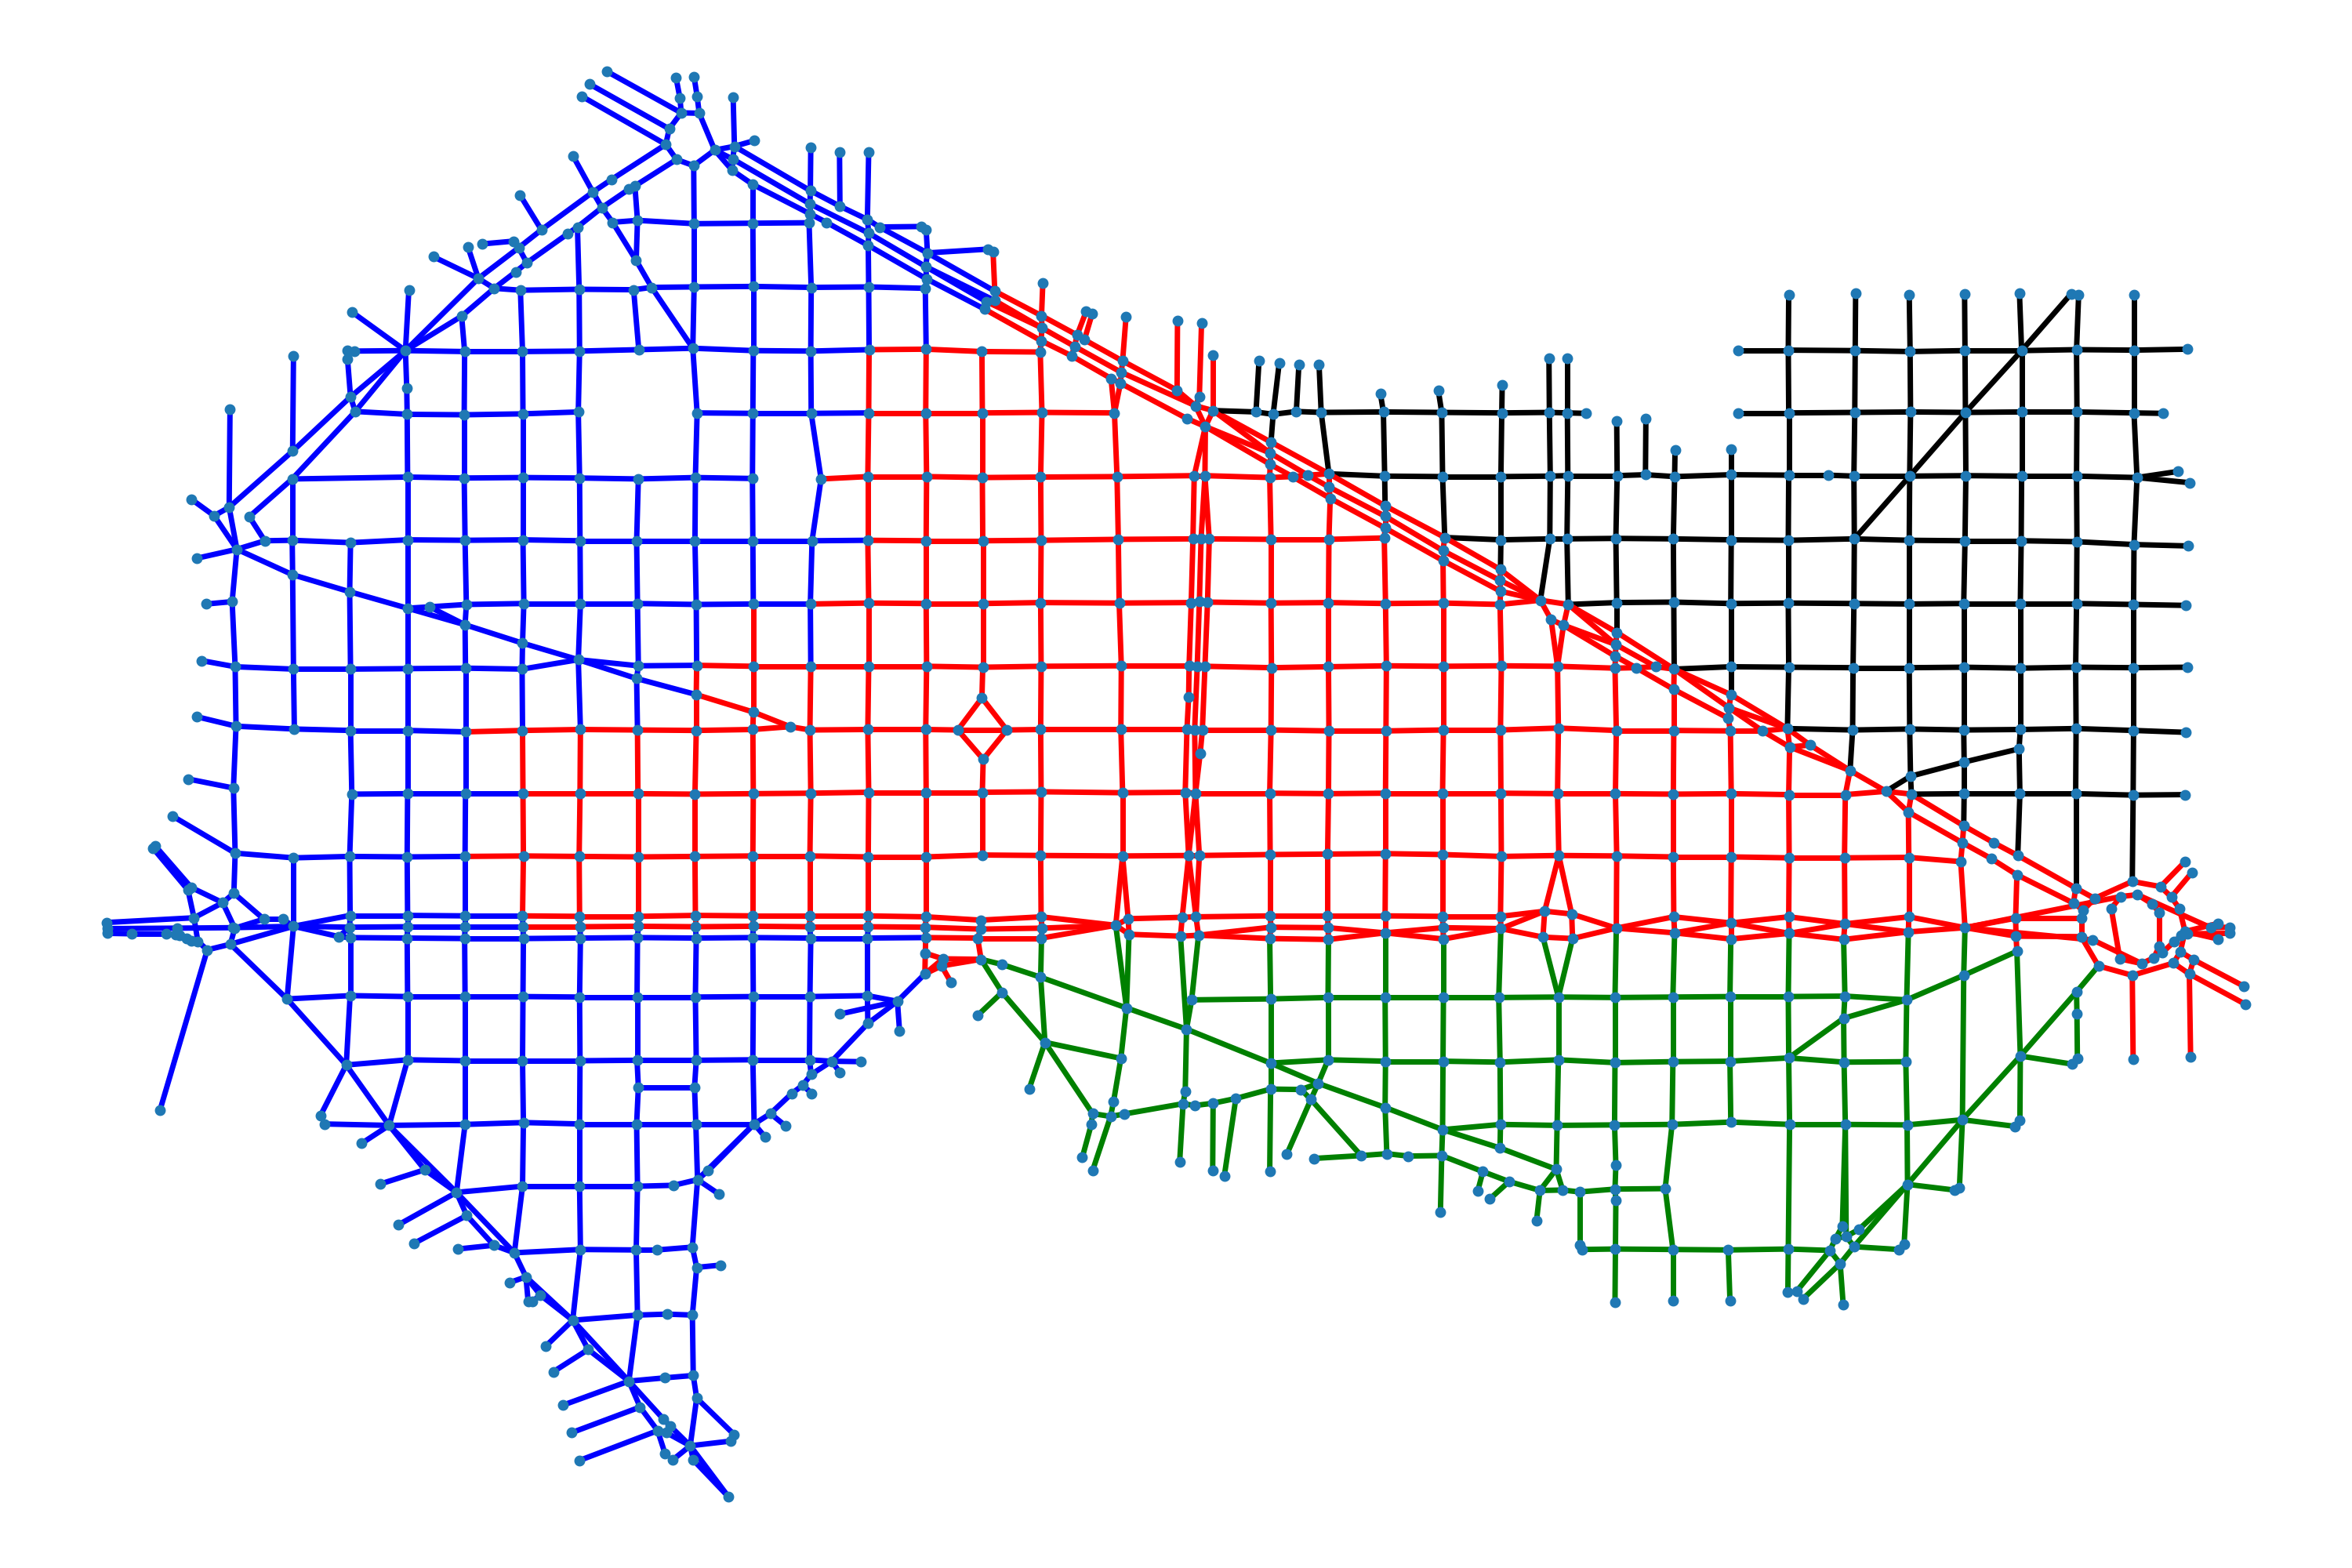
\includegraphics[width=10cm]{Images/Graph 4 regions.png}
        \caption{Separation of the network into four regions}
        \label{Separation of the network into four regions}
    \end{center}
\end{figure}


The data that are provided allow to describe the network with the position of each road, its length and the number of lanes. In addition, for each of the roads, the flow and occupancy were measured every 90 seconds over a period of 2 hours.\\
Based on all these data, it will be possible to study the congestion in the different regions according to the time period studied. It will also be possible to calculate other characteristic variables for the study of the network such as density, link speed, average speed or production and accumulation. It could then be interesting to study the system on the basis of these characteristics. Furthermore, in order to reduce the amount of data to be processed, it could be tried to select only some of the data and to compare the results to those for the whole data set. Different methods of data selection could then be studied to minimize the errors with respect to the basic data.


\section{Step 1 - Level of congestion in the network}

The first step is to create snapshots of the network. These graphs represent the level of congestion of each link at different times of the simulation.

The goal is to place the different nodes of the network, then link them according to the existing connections in reality. Finally, a gray-scale format must be used to represent the congestion level of the different links. 

A completely empty link will be completely white, while a completely congested link will be completely black. Between the two, a grey scale will be used to represent the occupancy rate of the different links of the network at different times of study.\\

The different graphs below represent the different occupations of the lanes at a given time, respectively 60, 90 and 120 minutes.
\begin{figure}[H]
    \begin{center}
        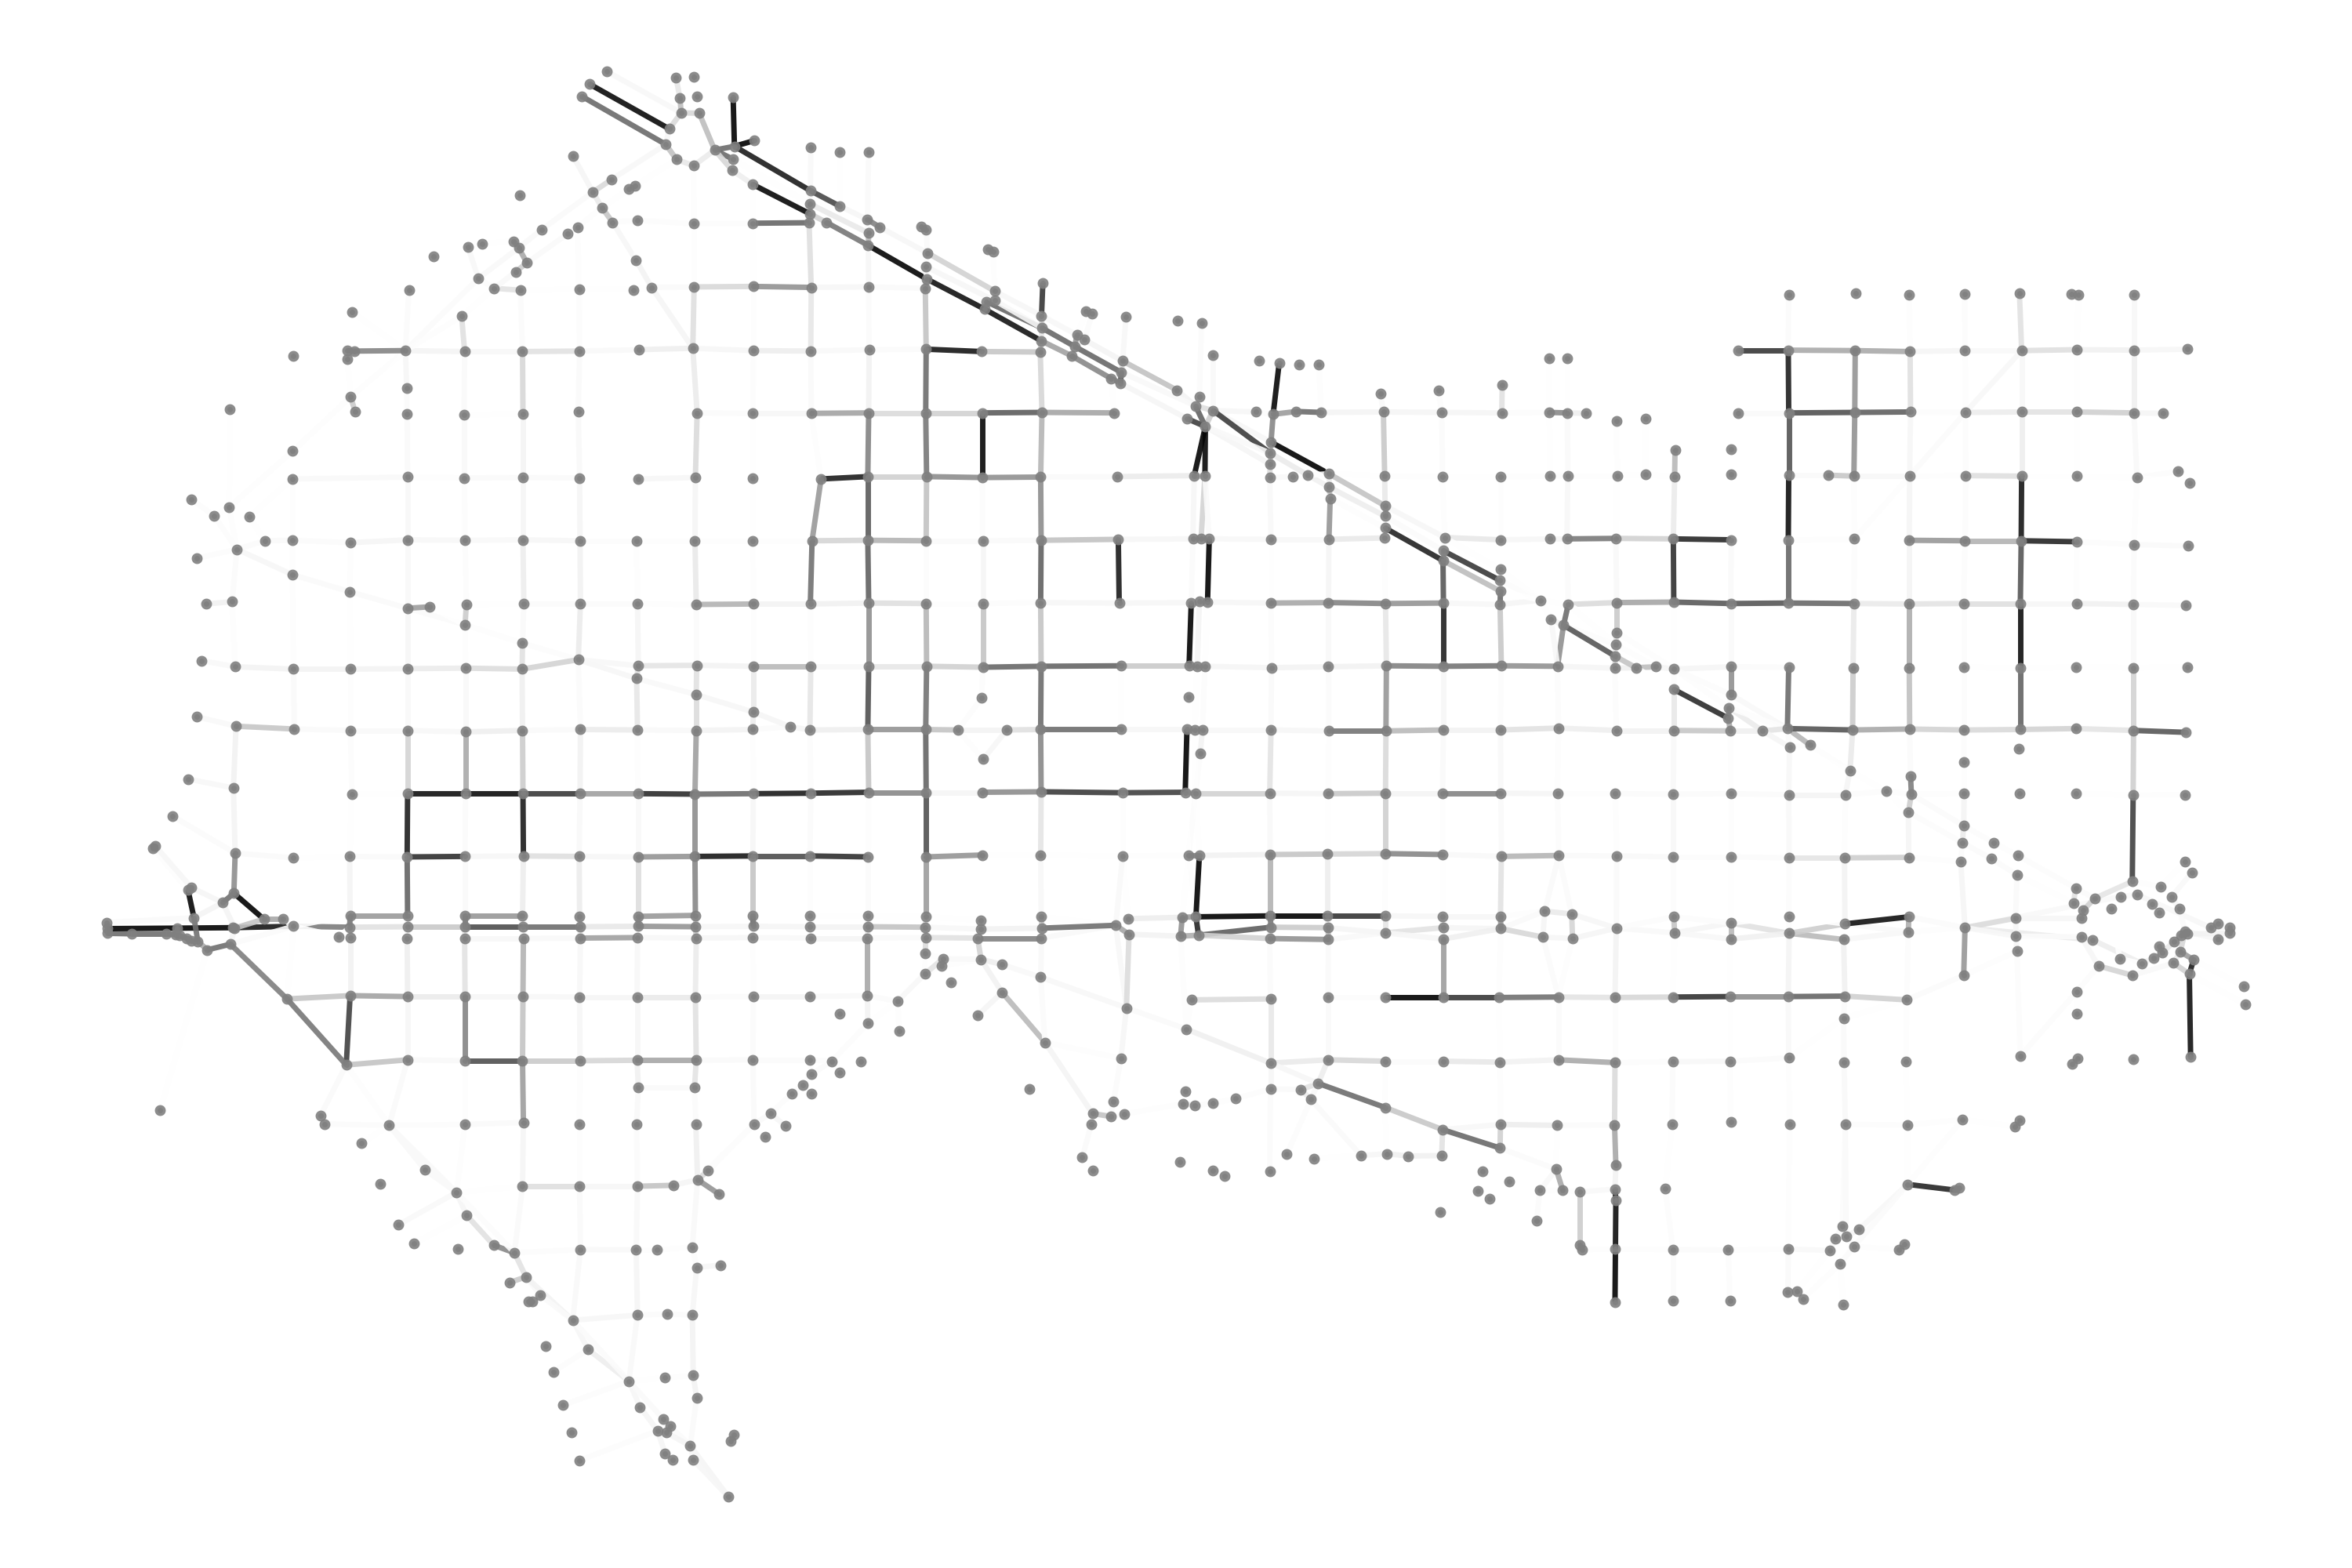
\includegraphics[width=9cm]{Images/Graph_gray_60min.png}
        \caption{Congestion level of each link at time 60 min}
        \label{Congestion level of each link at time 60 min}
    \end{center}
\end{figure}

\begin{figure}[H]
    \begin{center}
        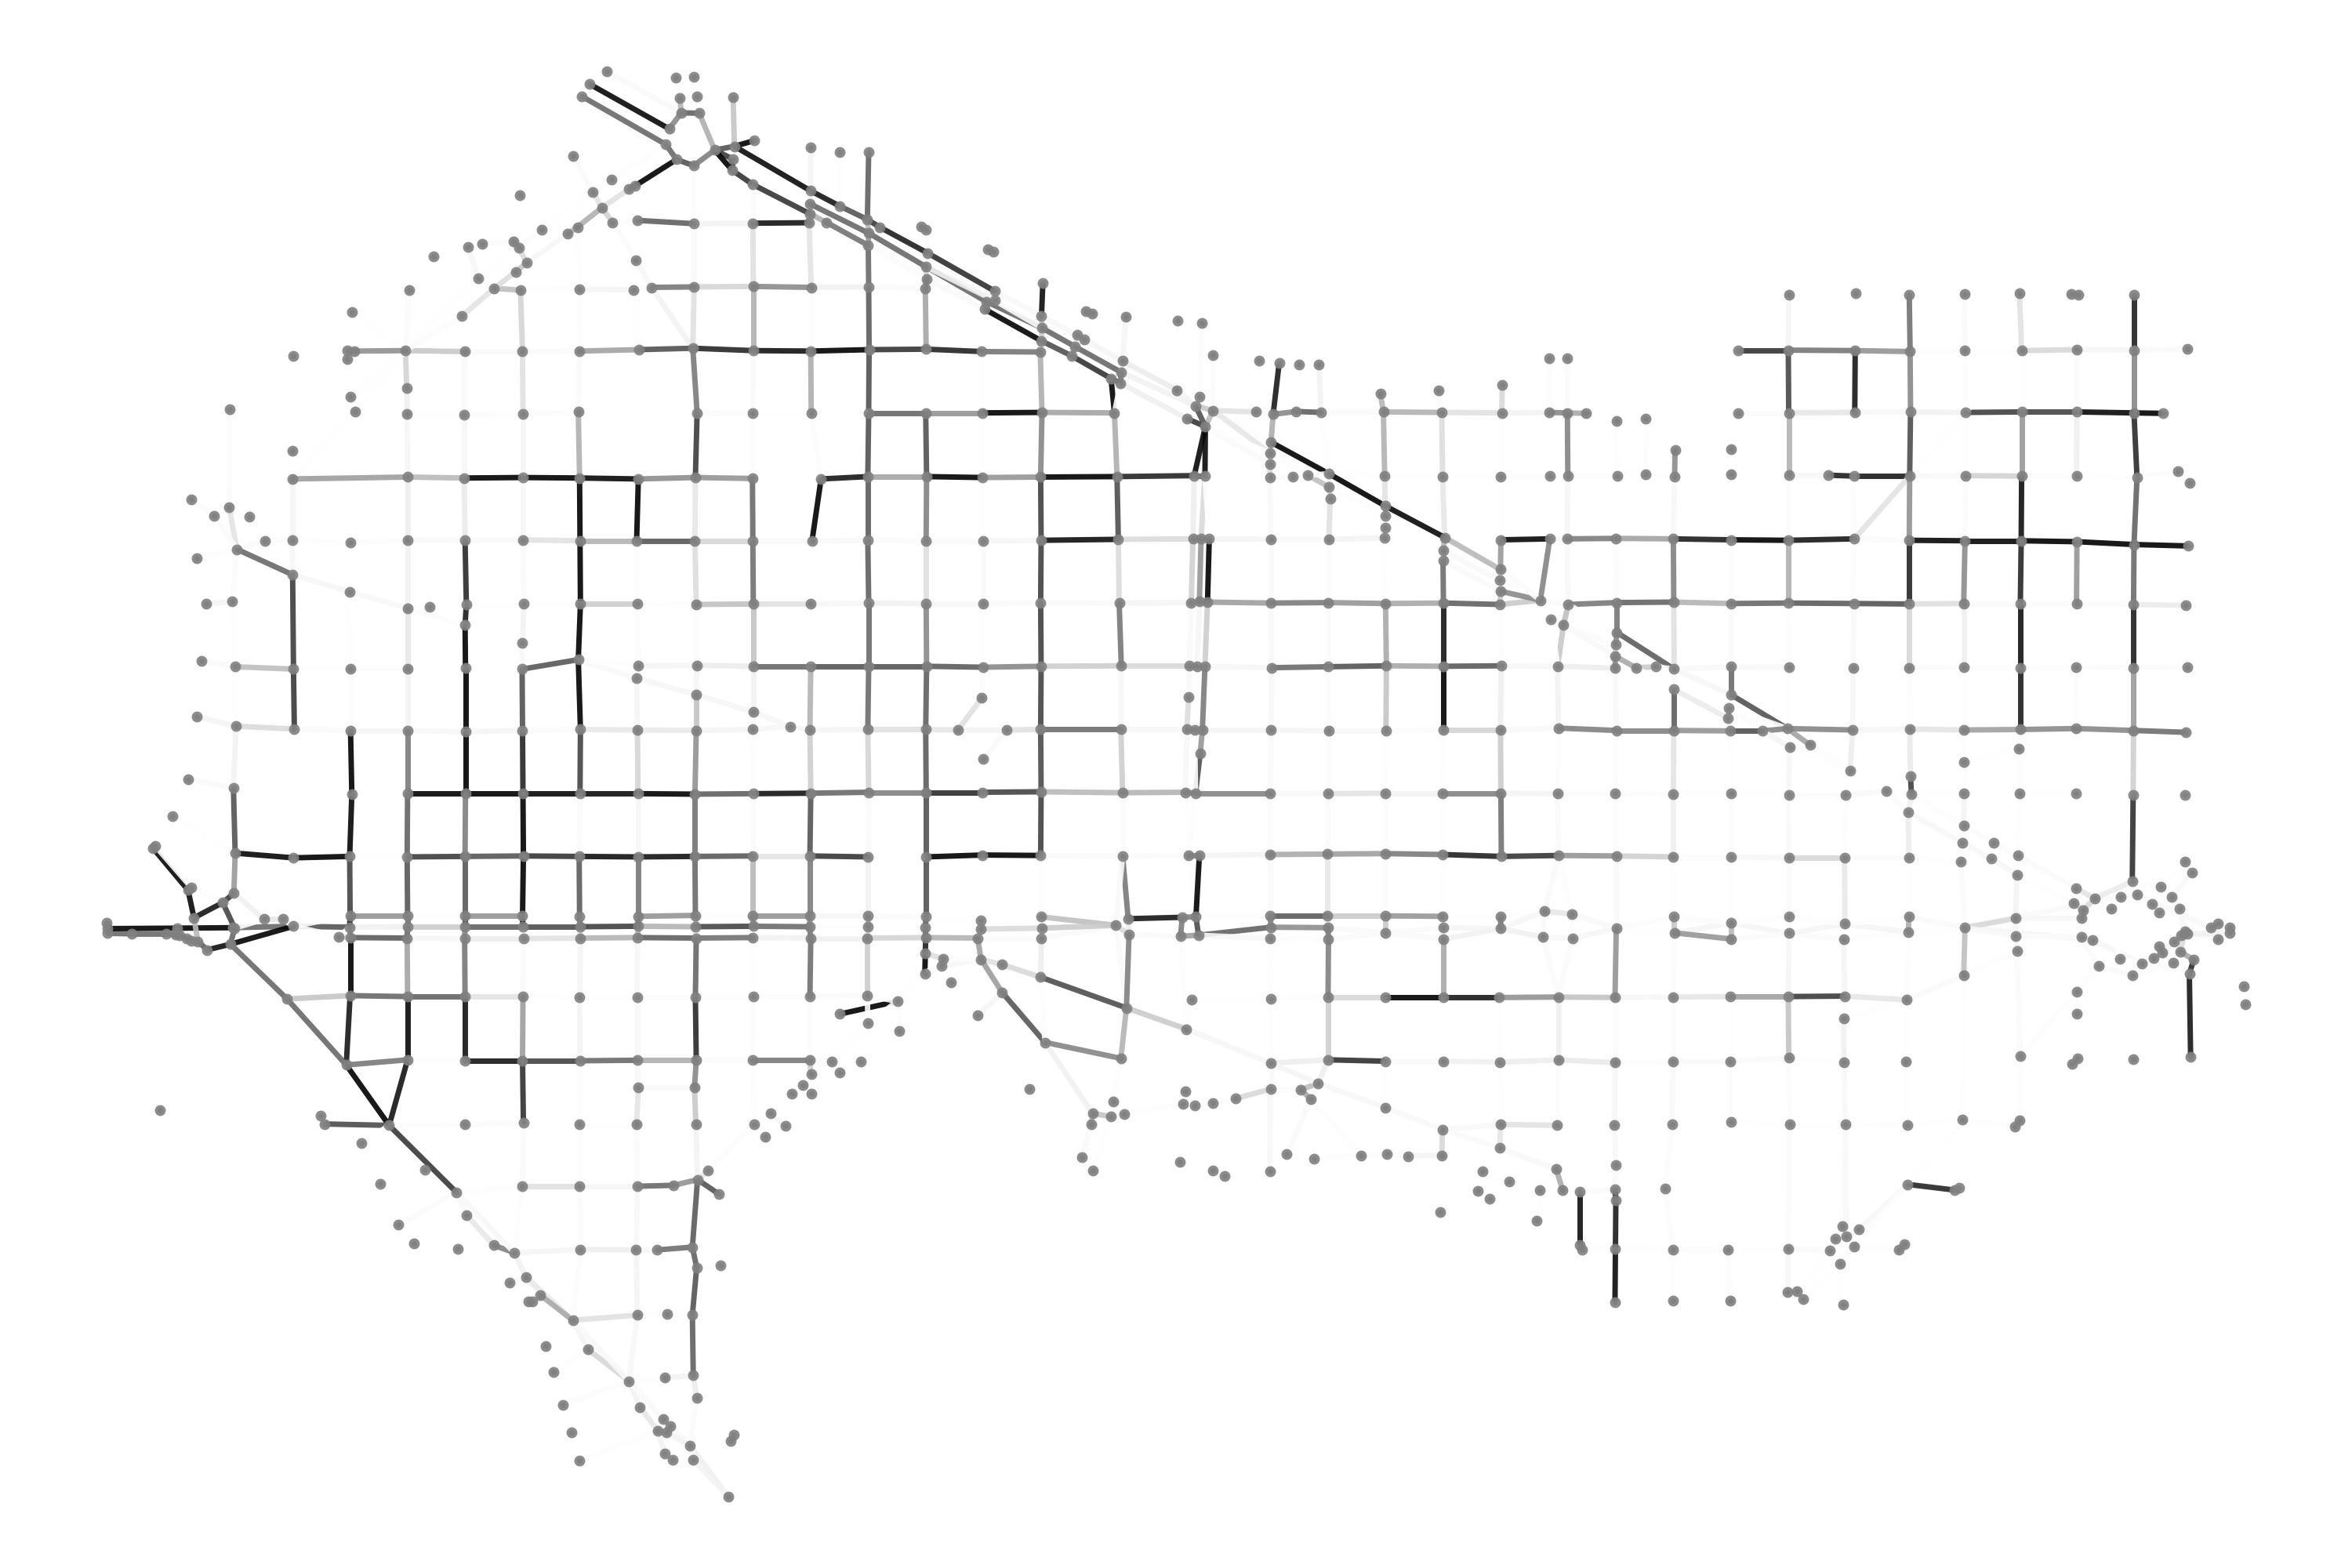
\includegraphics[width=9cm]{Images/Graph_gray_90min.png}
        \caption{Congestion level of each link at time 90 min}
        \label{Congestion level of each link at time 90 min}
    \end{center}
\end{figure}

\begin{figure}[H]
    \begin{center}
        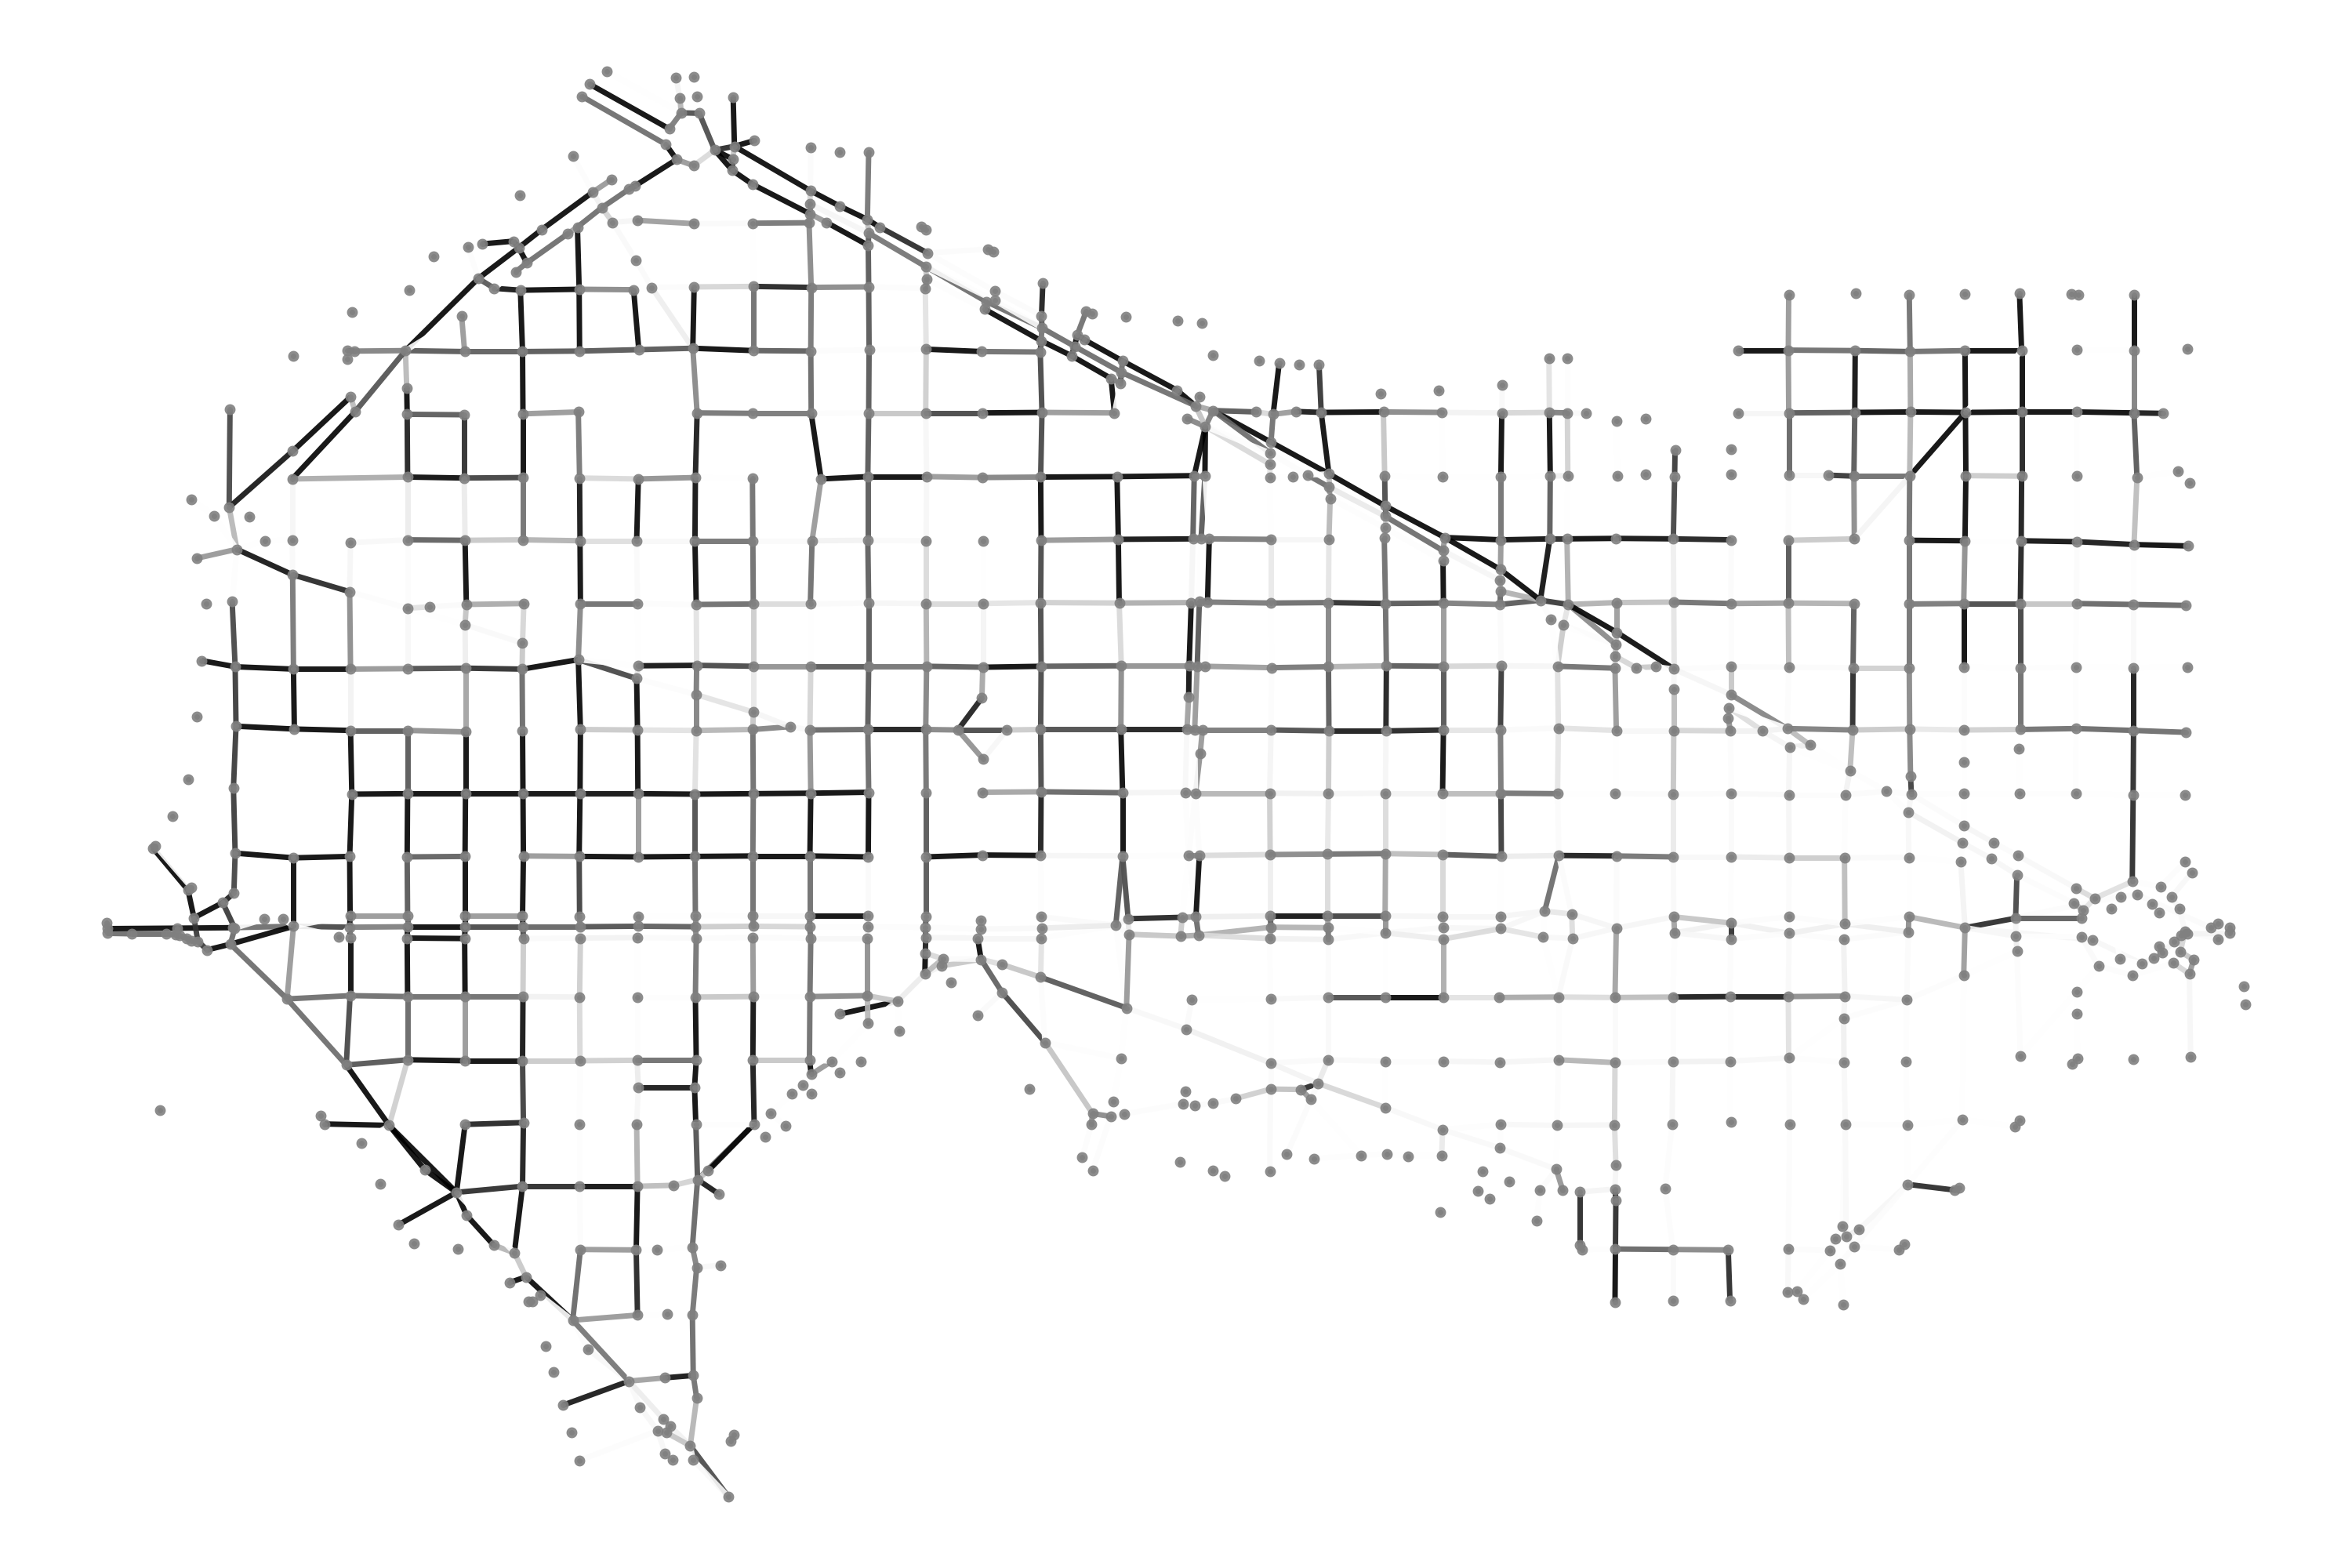
\includegraphics[width=9cm]{Images/Graph_gray_120min.png}
        \caption{Congestion level of each link at time 120 min}
        \label{Congestion level of each link at time 120 min}
    \end{center}
\end{figure}

\bigbreak
\newpage
Let's talk about the different graphs above and the conclusions that can be drawn from them. 
First of all, after 60 minutes, the level of congestion remains rather low on the whole network, but not insignificant however. Some lanes seem to be slightly congested, but overall, a large majority seem to be almost empty.\\
Secondly, looking more closely at the graph representing the network after 90 minutes, congestion still seems relatively moderate, but increasing. Indeed, there are more links that appear to be full than 30 minutes earlier. This could be due to a number of factors, whether it is an increase in demand, but also possibly external factors that reduce capacity such as an accident. However, as the increase in congestion does not seem to be particularly localised but rather takes place across the whole network, an increase in demand seems more likely. It is then interesting to see if this trend is confirmed 30 minutes later. \\
Finally, after 120 minutes, the observation made after 90 minutes is confirmed. An increase in congestion is noted at various points in the network, both in the centre and in the periphery.

\smallbreak

In summary, it is possible to note a fairly significant increase in the overall level of congestion in the network. As this increase seems to be rather spread out, it probably looks like an overall increase in demand and thus in the number of vehicles in the network.\\
This increase can occur in a number of ways. However, a rather plausible assumption that can be made in this case is that these are early morning measures. At the beginning, few people frequent the network and congestion is thus rather reduced. However, as time goes on, the rush hour is approaching and a lot of people are going to the city centre to work. As a result, demand is high and the level of congestion on the network increases. \\
If this assumption is correct, it would be likely that a decrease in congestion levels would occur later, once the worker's peak hour has passed. However, this is only one possible assumption to explain the evolution of congestion based on 3 graphs, but other assumptions are also entirely possible.

\bigbreak
\bigbreak
\bigbreak

\section{Step 2 - Volume vs. average occupancy}
Firstly, the different volumes are given in number of vehicles per link. This is transformed into a number of vehicles per hour for each time step on each link (normalise by 90 seconds per hour, factor 40 between the 2).

Then, the different occupancy, which correspond to the fraction of the time when the loop detector is occupied, and therefore volume in vehicles per hour are known. This involves making scatter plots of volume vs occupancy for different cases (1 link, 2 links and the whole network). 

Afterwards, it will be necessary to extract the links according to the different regions and make the same graphs. It will then be interesting to see to what extent the different data sets will influence the scatter measurements and the results obtained.\\ 

\begin{figure}[H]
    \begin{center}
        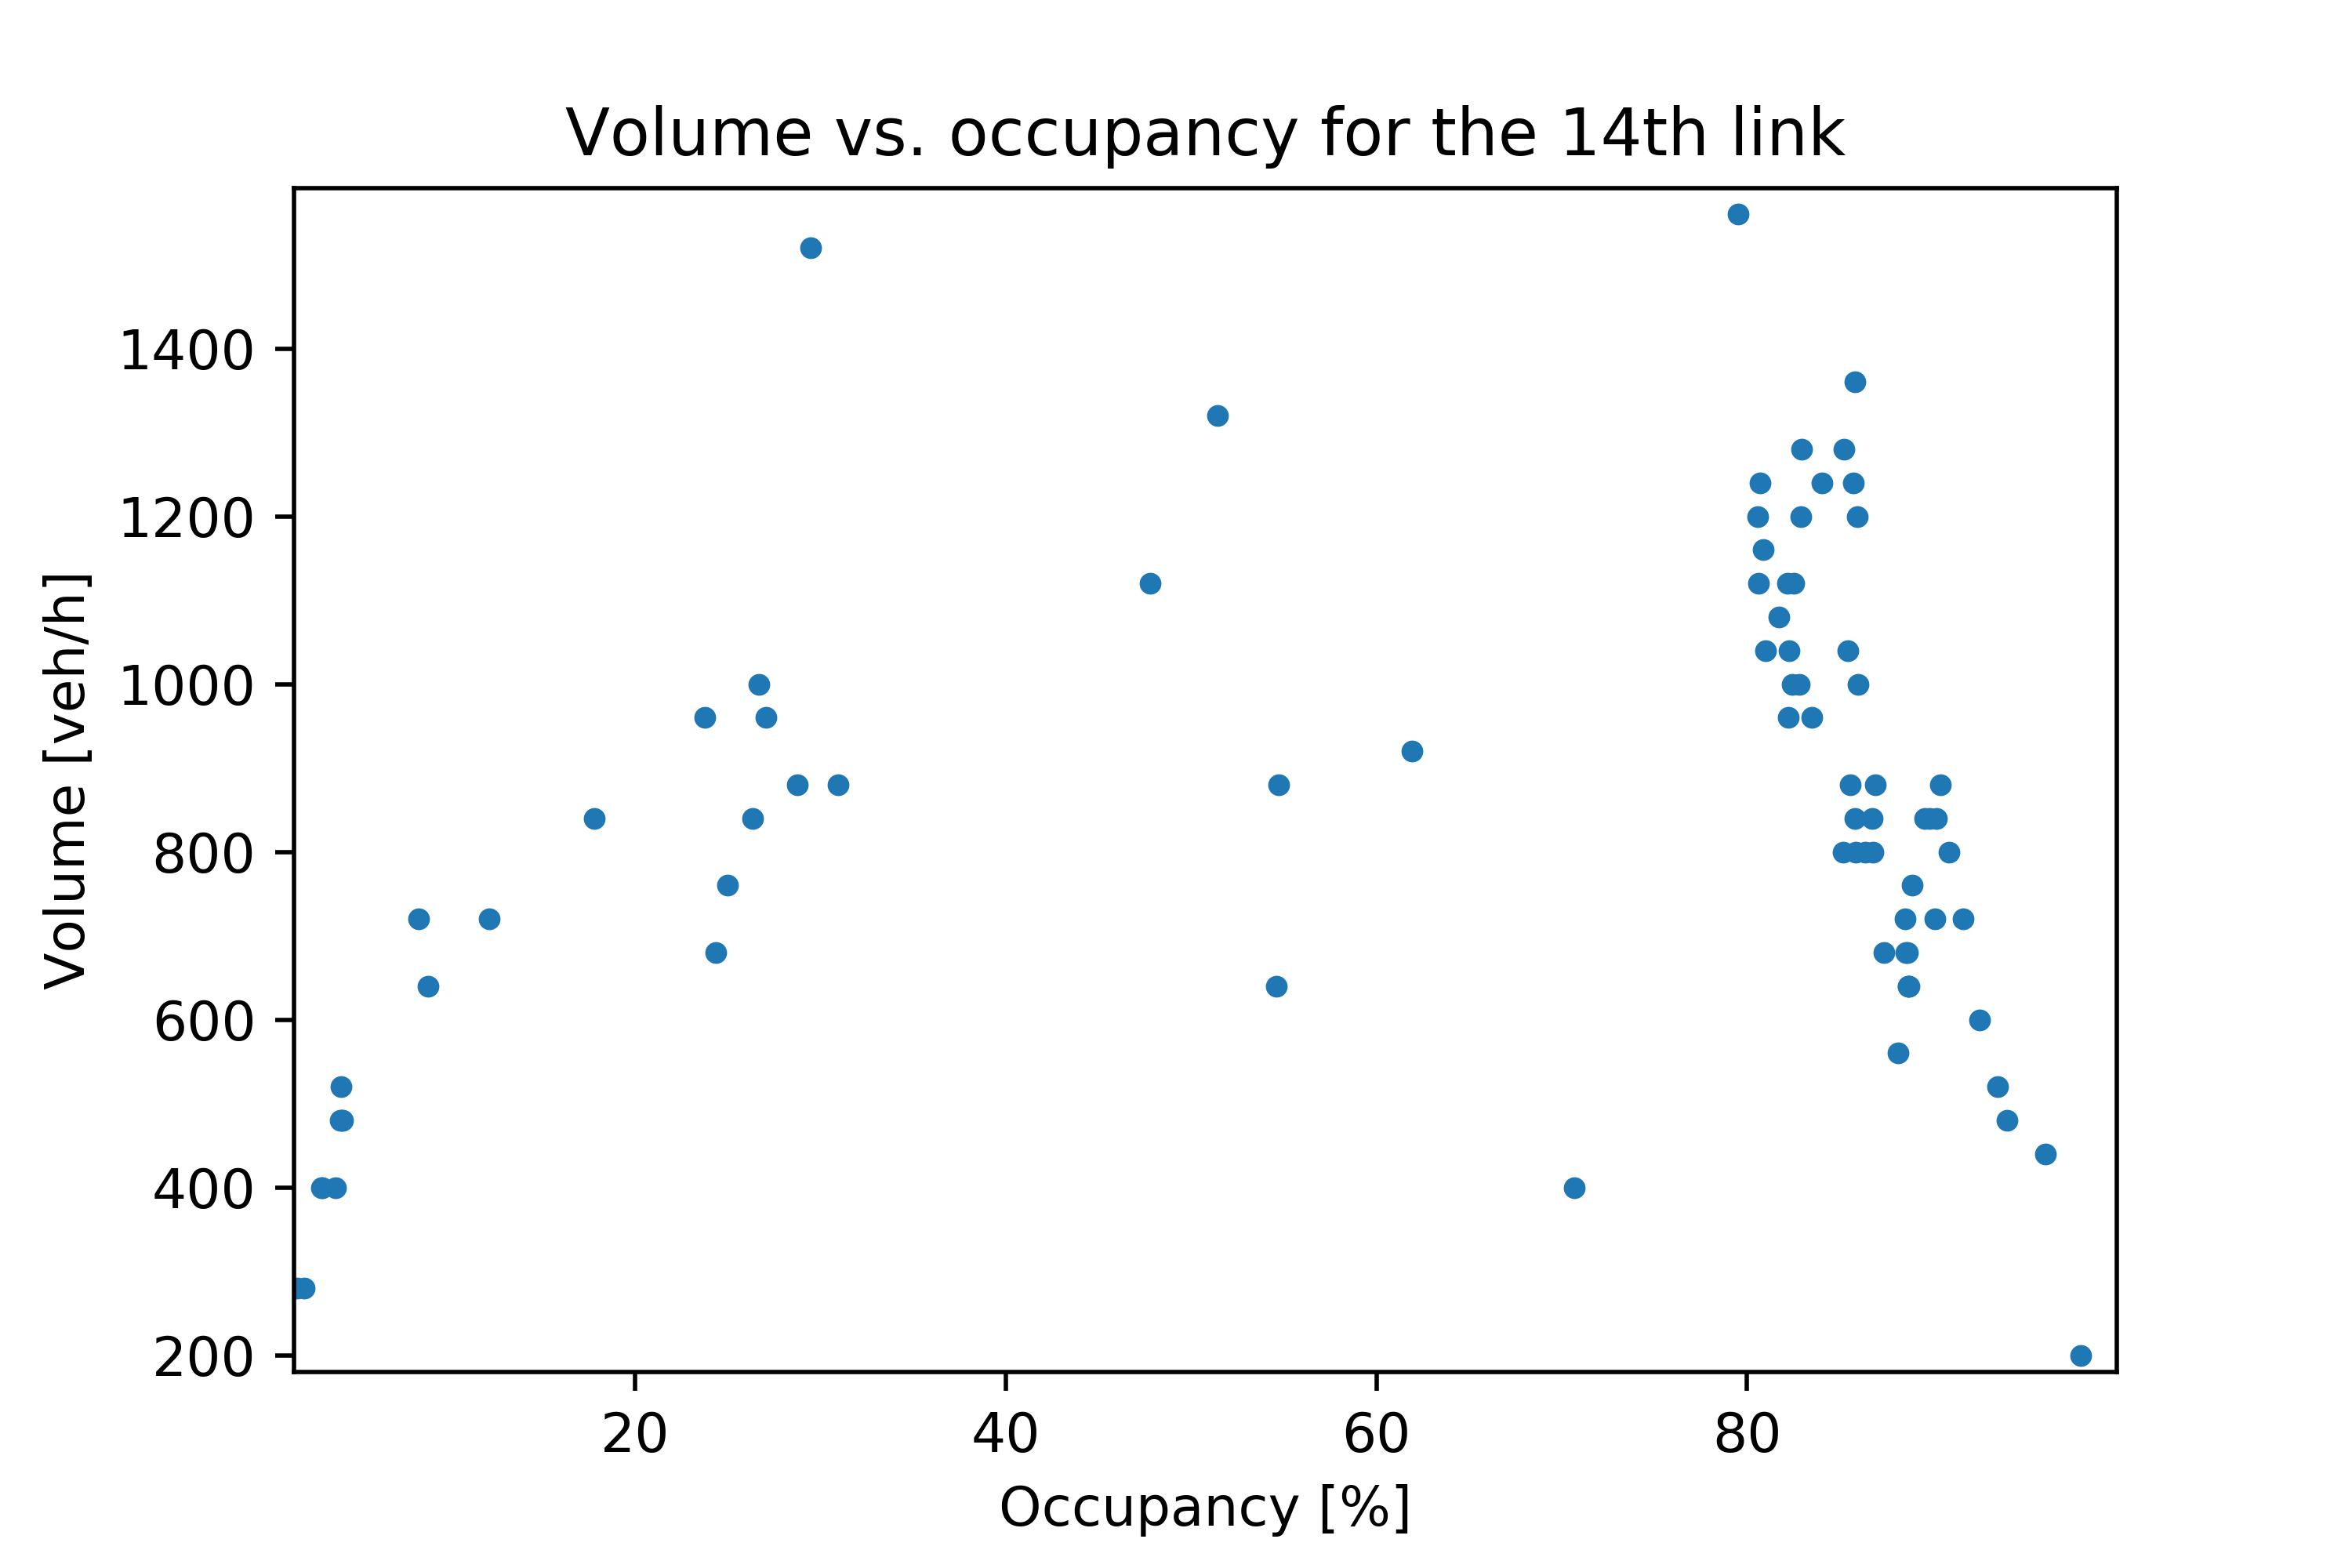
\includegraphics[width=9cm]{Images/Volume vs. occupancy for the 90-seconds intervals for the 14th link.png}
        \caption{Volume vs. occupancy for the 90-seconds intervals for the 14th link}
        \label{Volume vs. occupancy for the 90-seconds intervals for the 14th link}
    \end{center}
\end{figure}

\begin{figure}[H]
    \begin{center}
        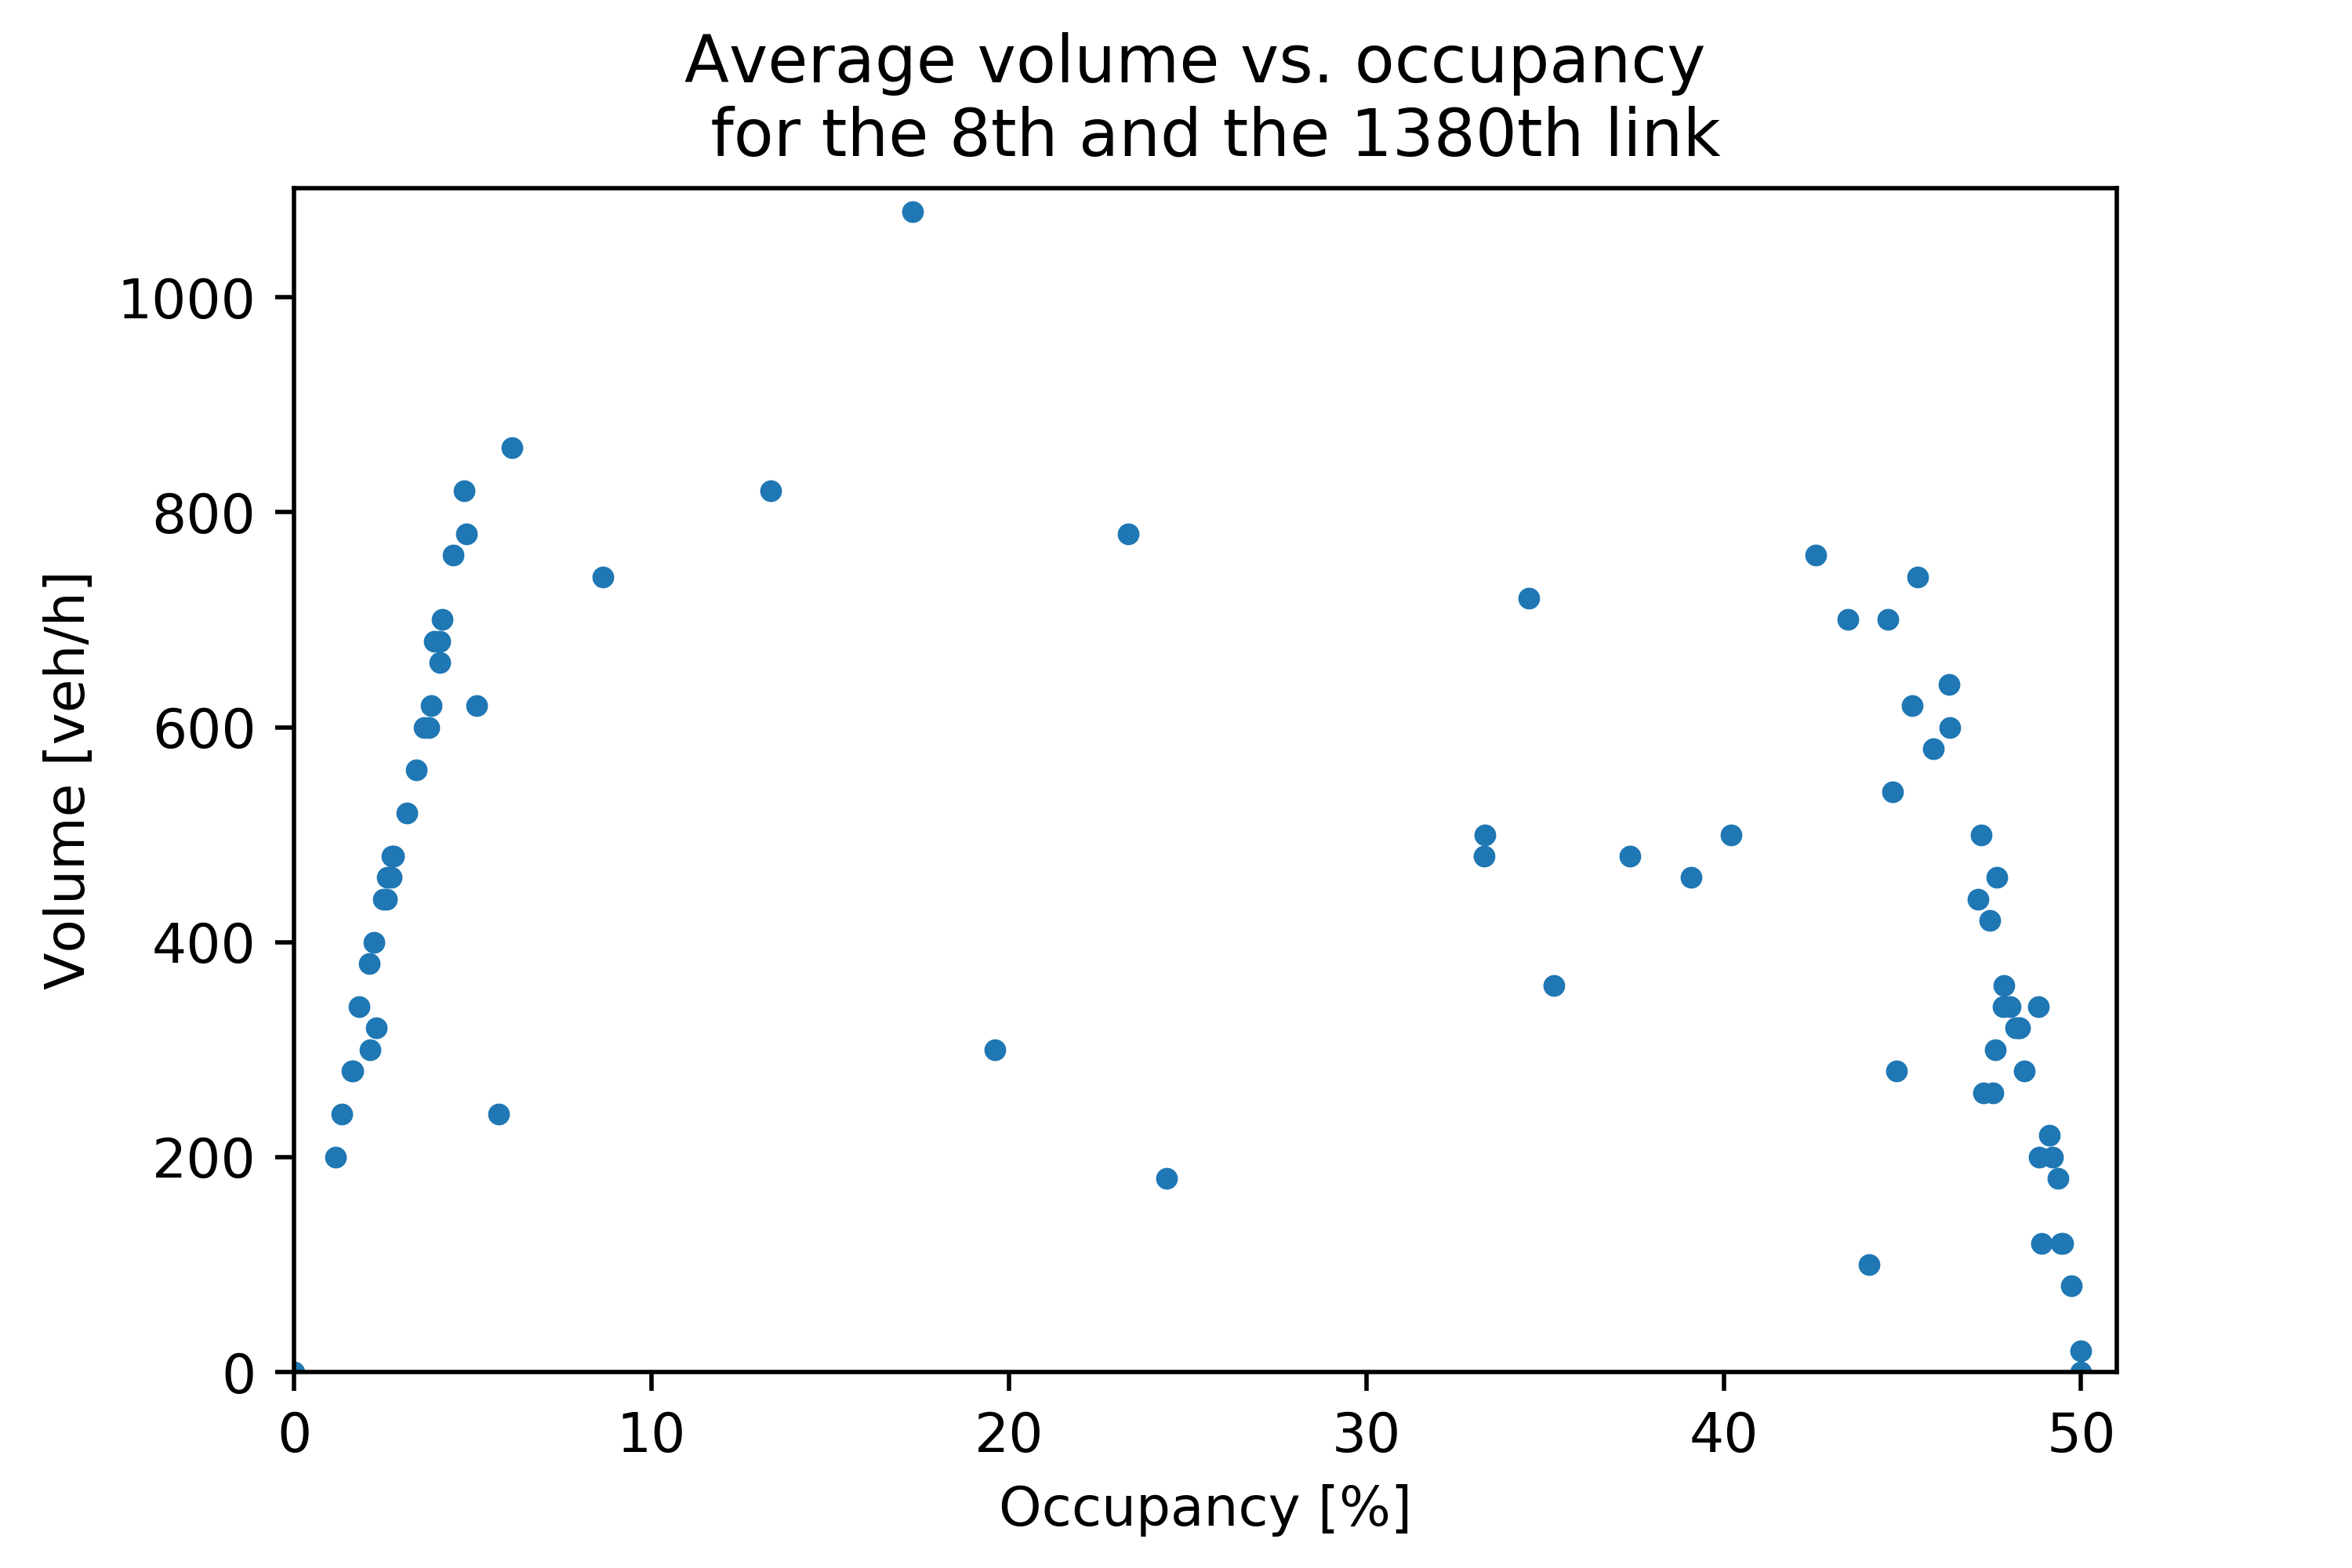
\includegraphics[width=9cm]{Images/Volume vs. occupancy for the 90-seconds intervals for the 8th and the 1380th link.png}
        \caption{Average volume vs. occupancy for the 90-seconds intervals for the 8th and the 1380th links}
        \label{Average volume vs. occupancy for the 90-seconds intervals for the 8th and the 1380th links}
    \end{center}
\end{figure}

\begin{figure}[H]
    \begin{center}
        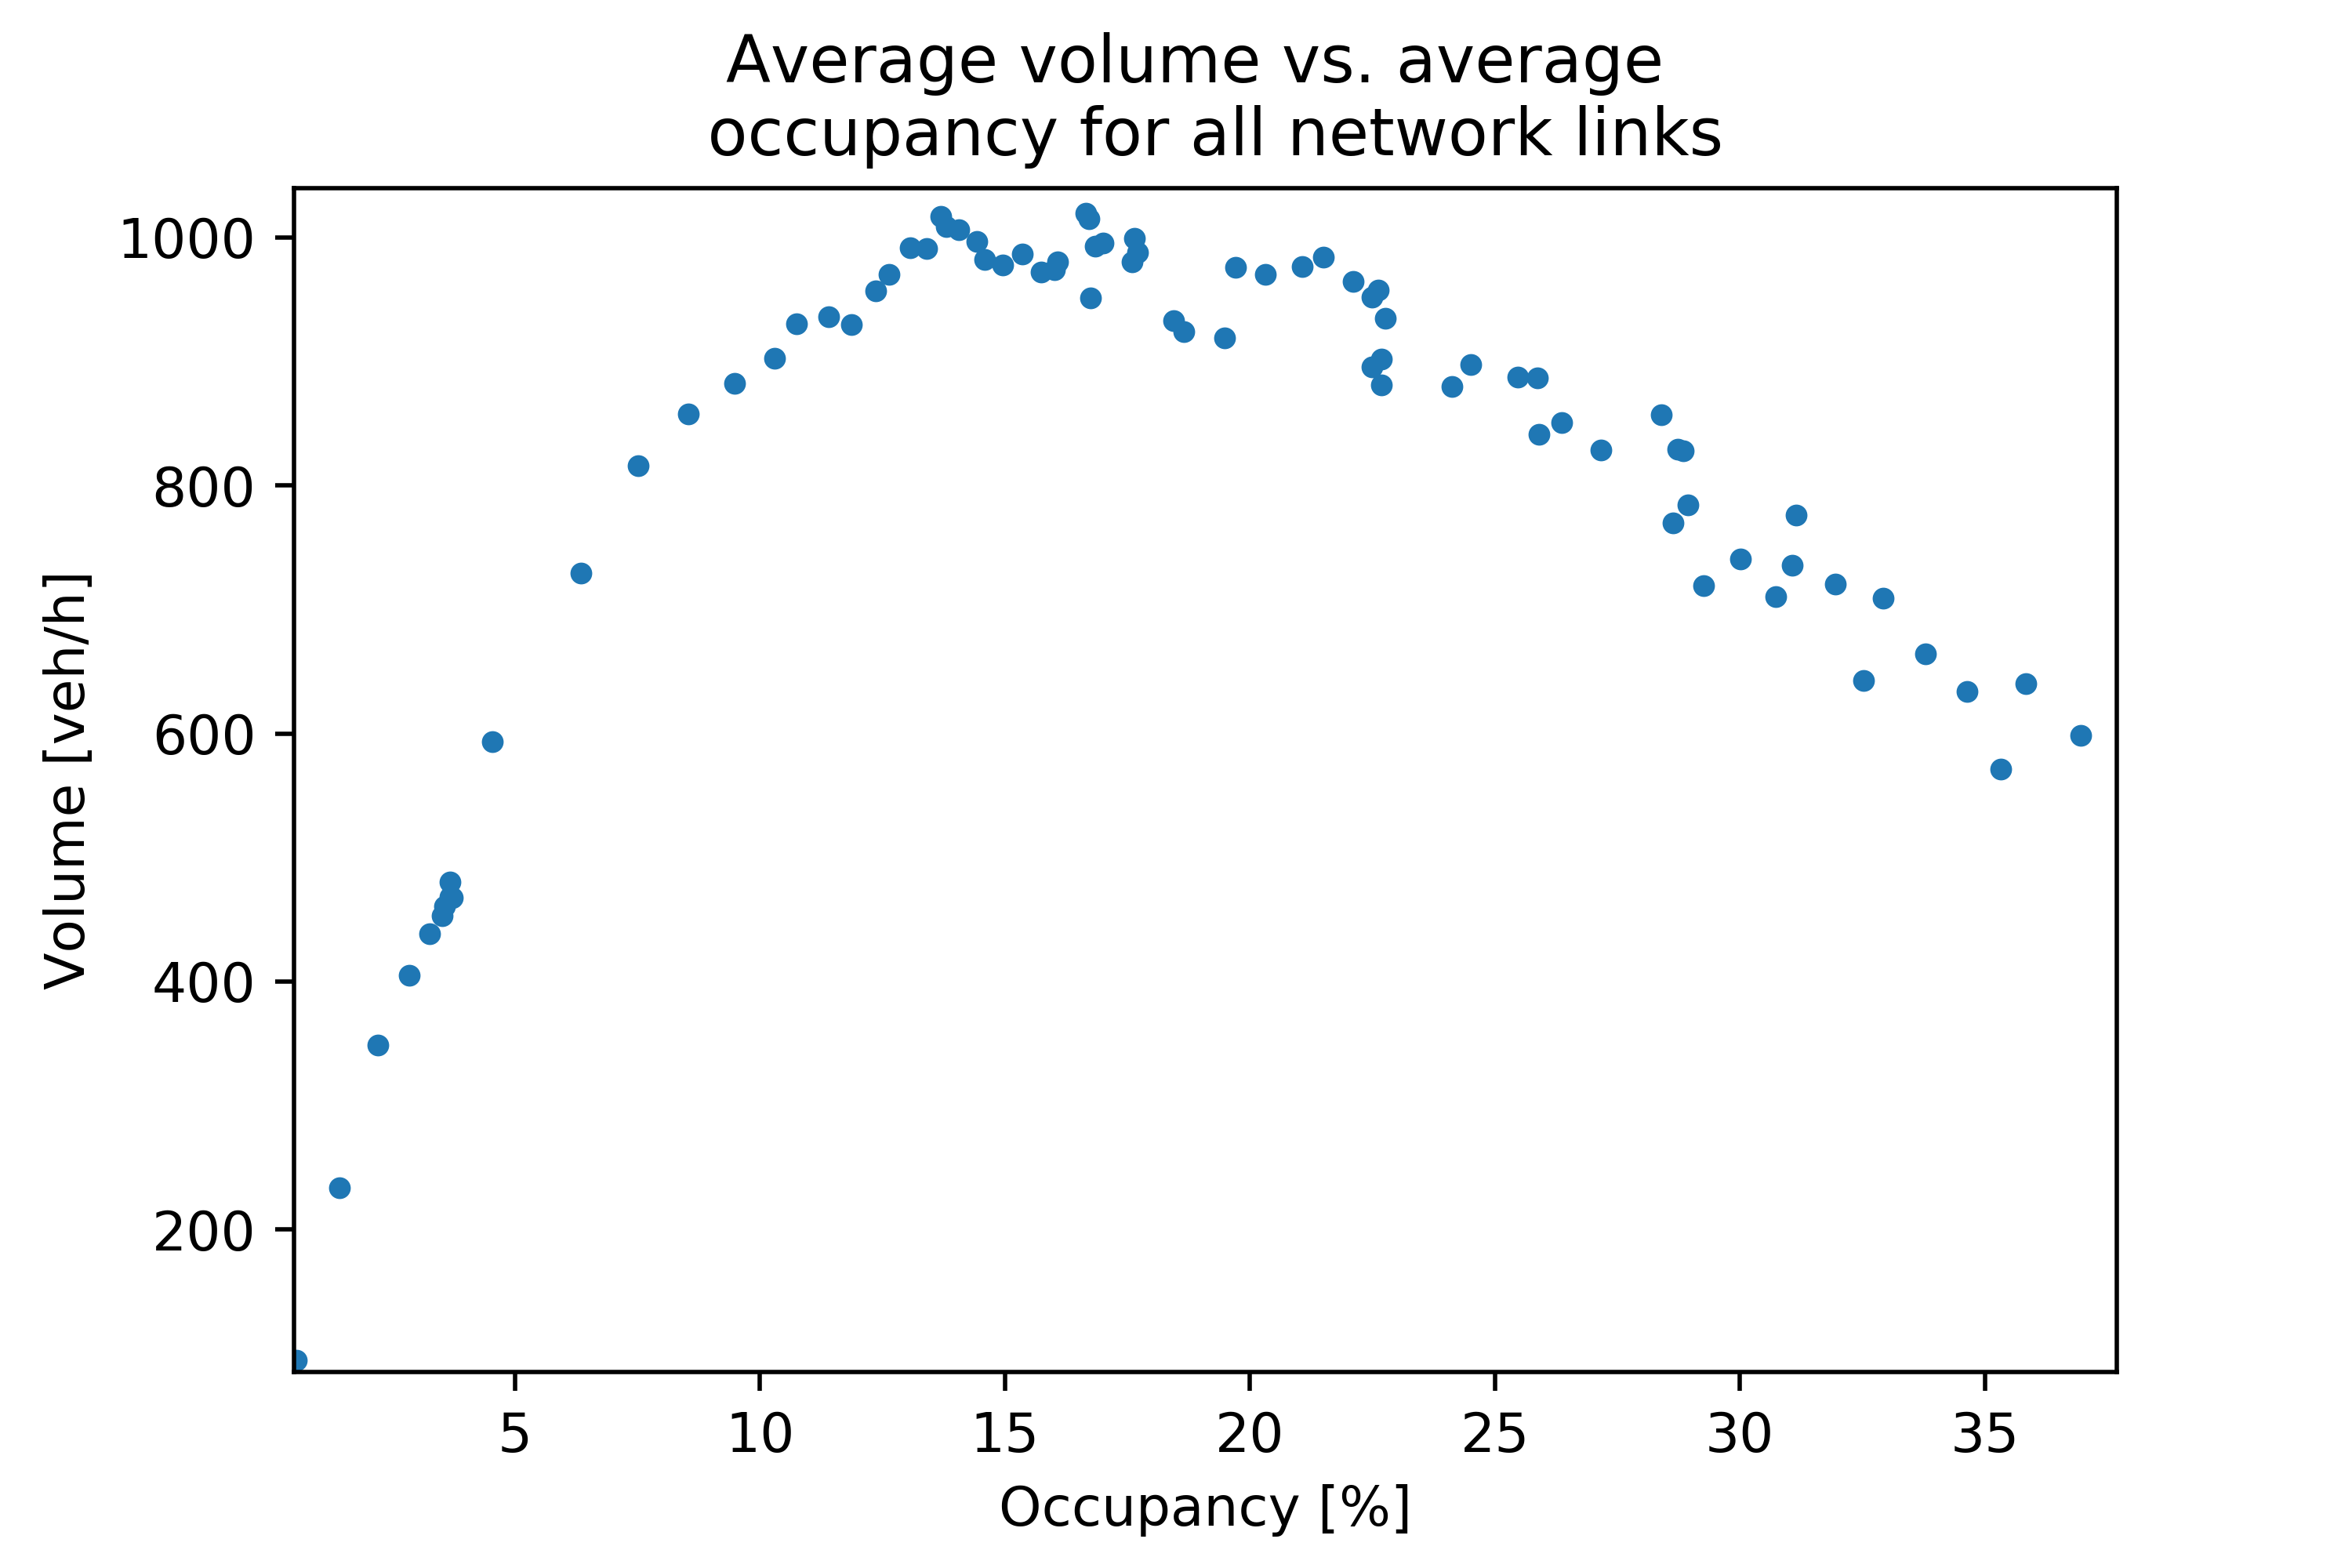
\includegraphics[width=9cm]{Images/Average volume vs. average occupancy for all network links.png}
        \caption{Average volume vs. average occupancy for all network links}
        \label{Average volume vs. average occupancy for all network links}
    \end{center}
\end{figure}

\begin{figure}[H]
    \begin{center}
        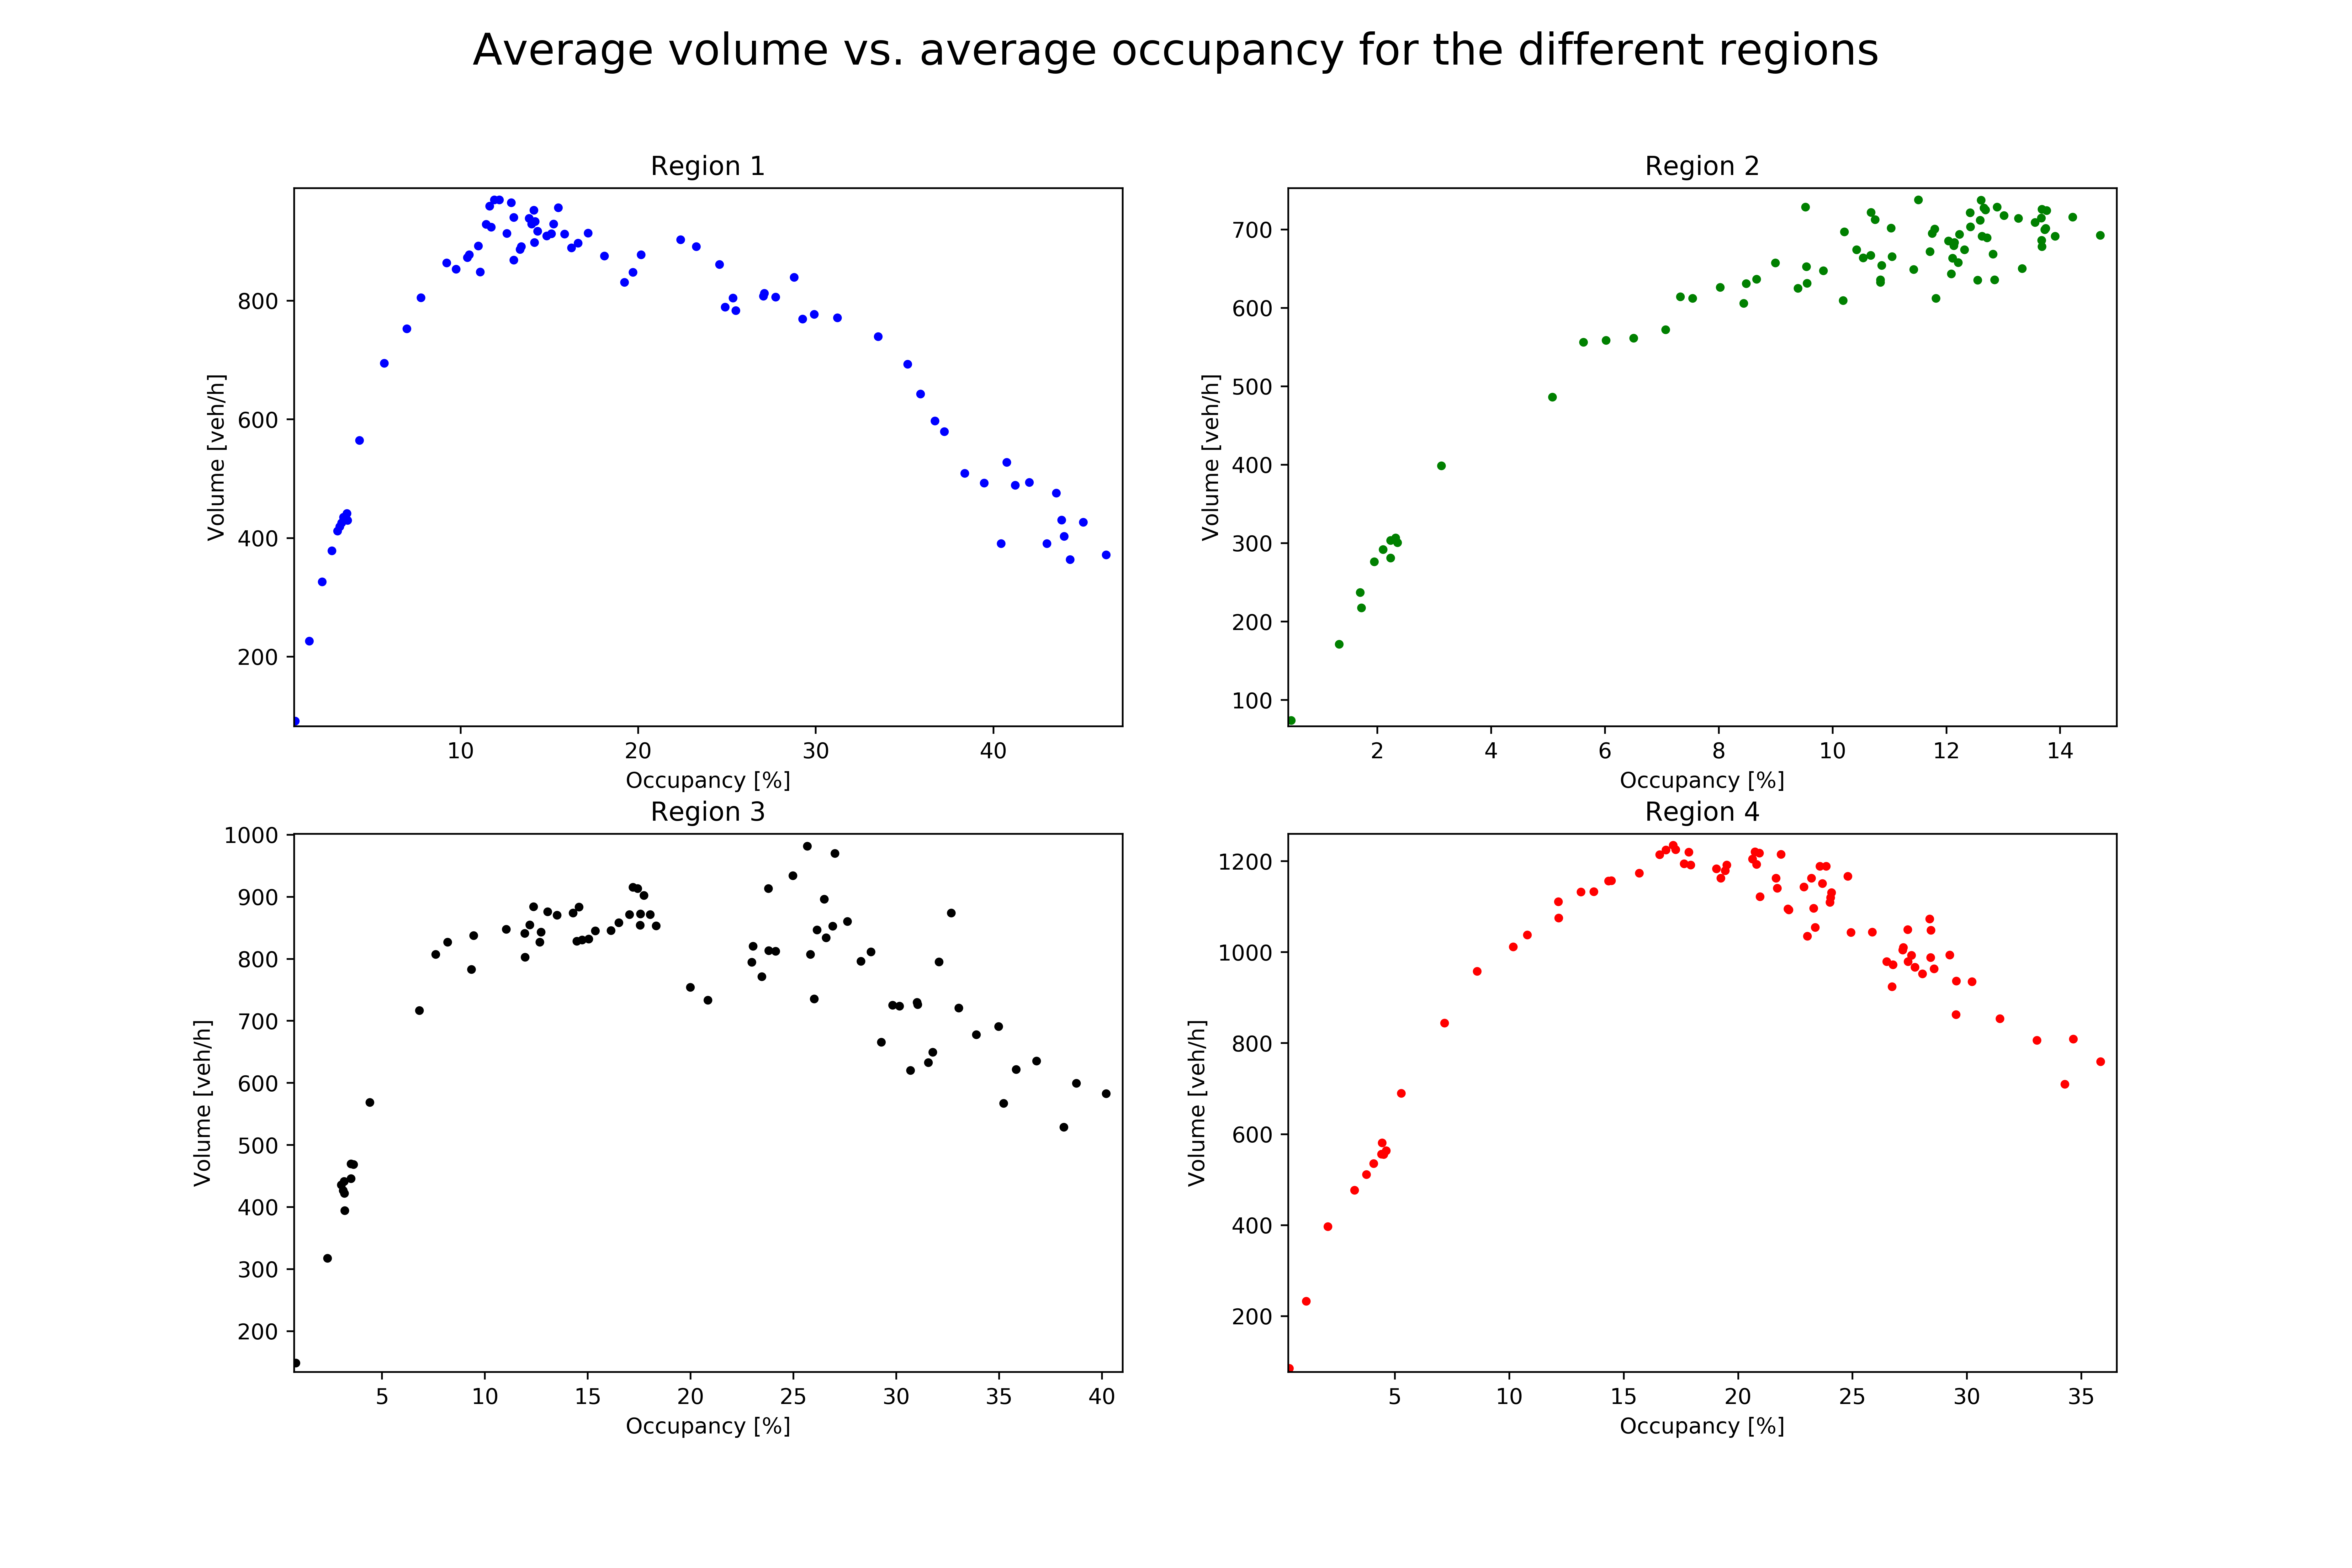
\includegraphics[width=18cm]{Images/Average volume vs. average occupancy for the 4 regions separatly.png}
        \caption{Average volume vs. average occupancy for the 4 regions separately}
        \label{Average volume vs. average occupancy for the 4 regions separately}
    \end{center}
\end{figure}

In order to get a better idea of the different cases and the variations between sets, it is interesting to visualise the different curves on the same graph, as seen below.\\
\begin{figure}[H]
    \begin{center}
        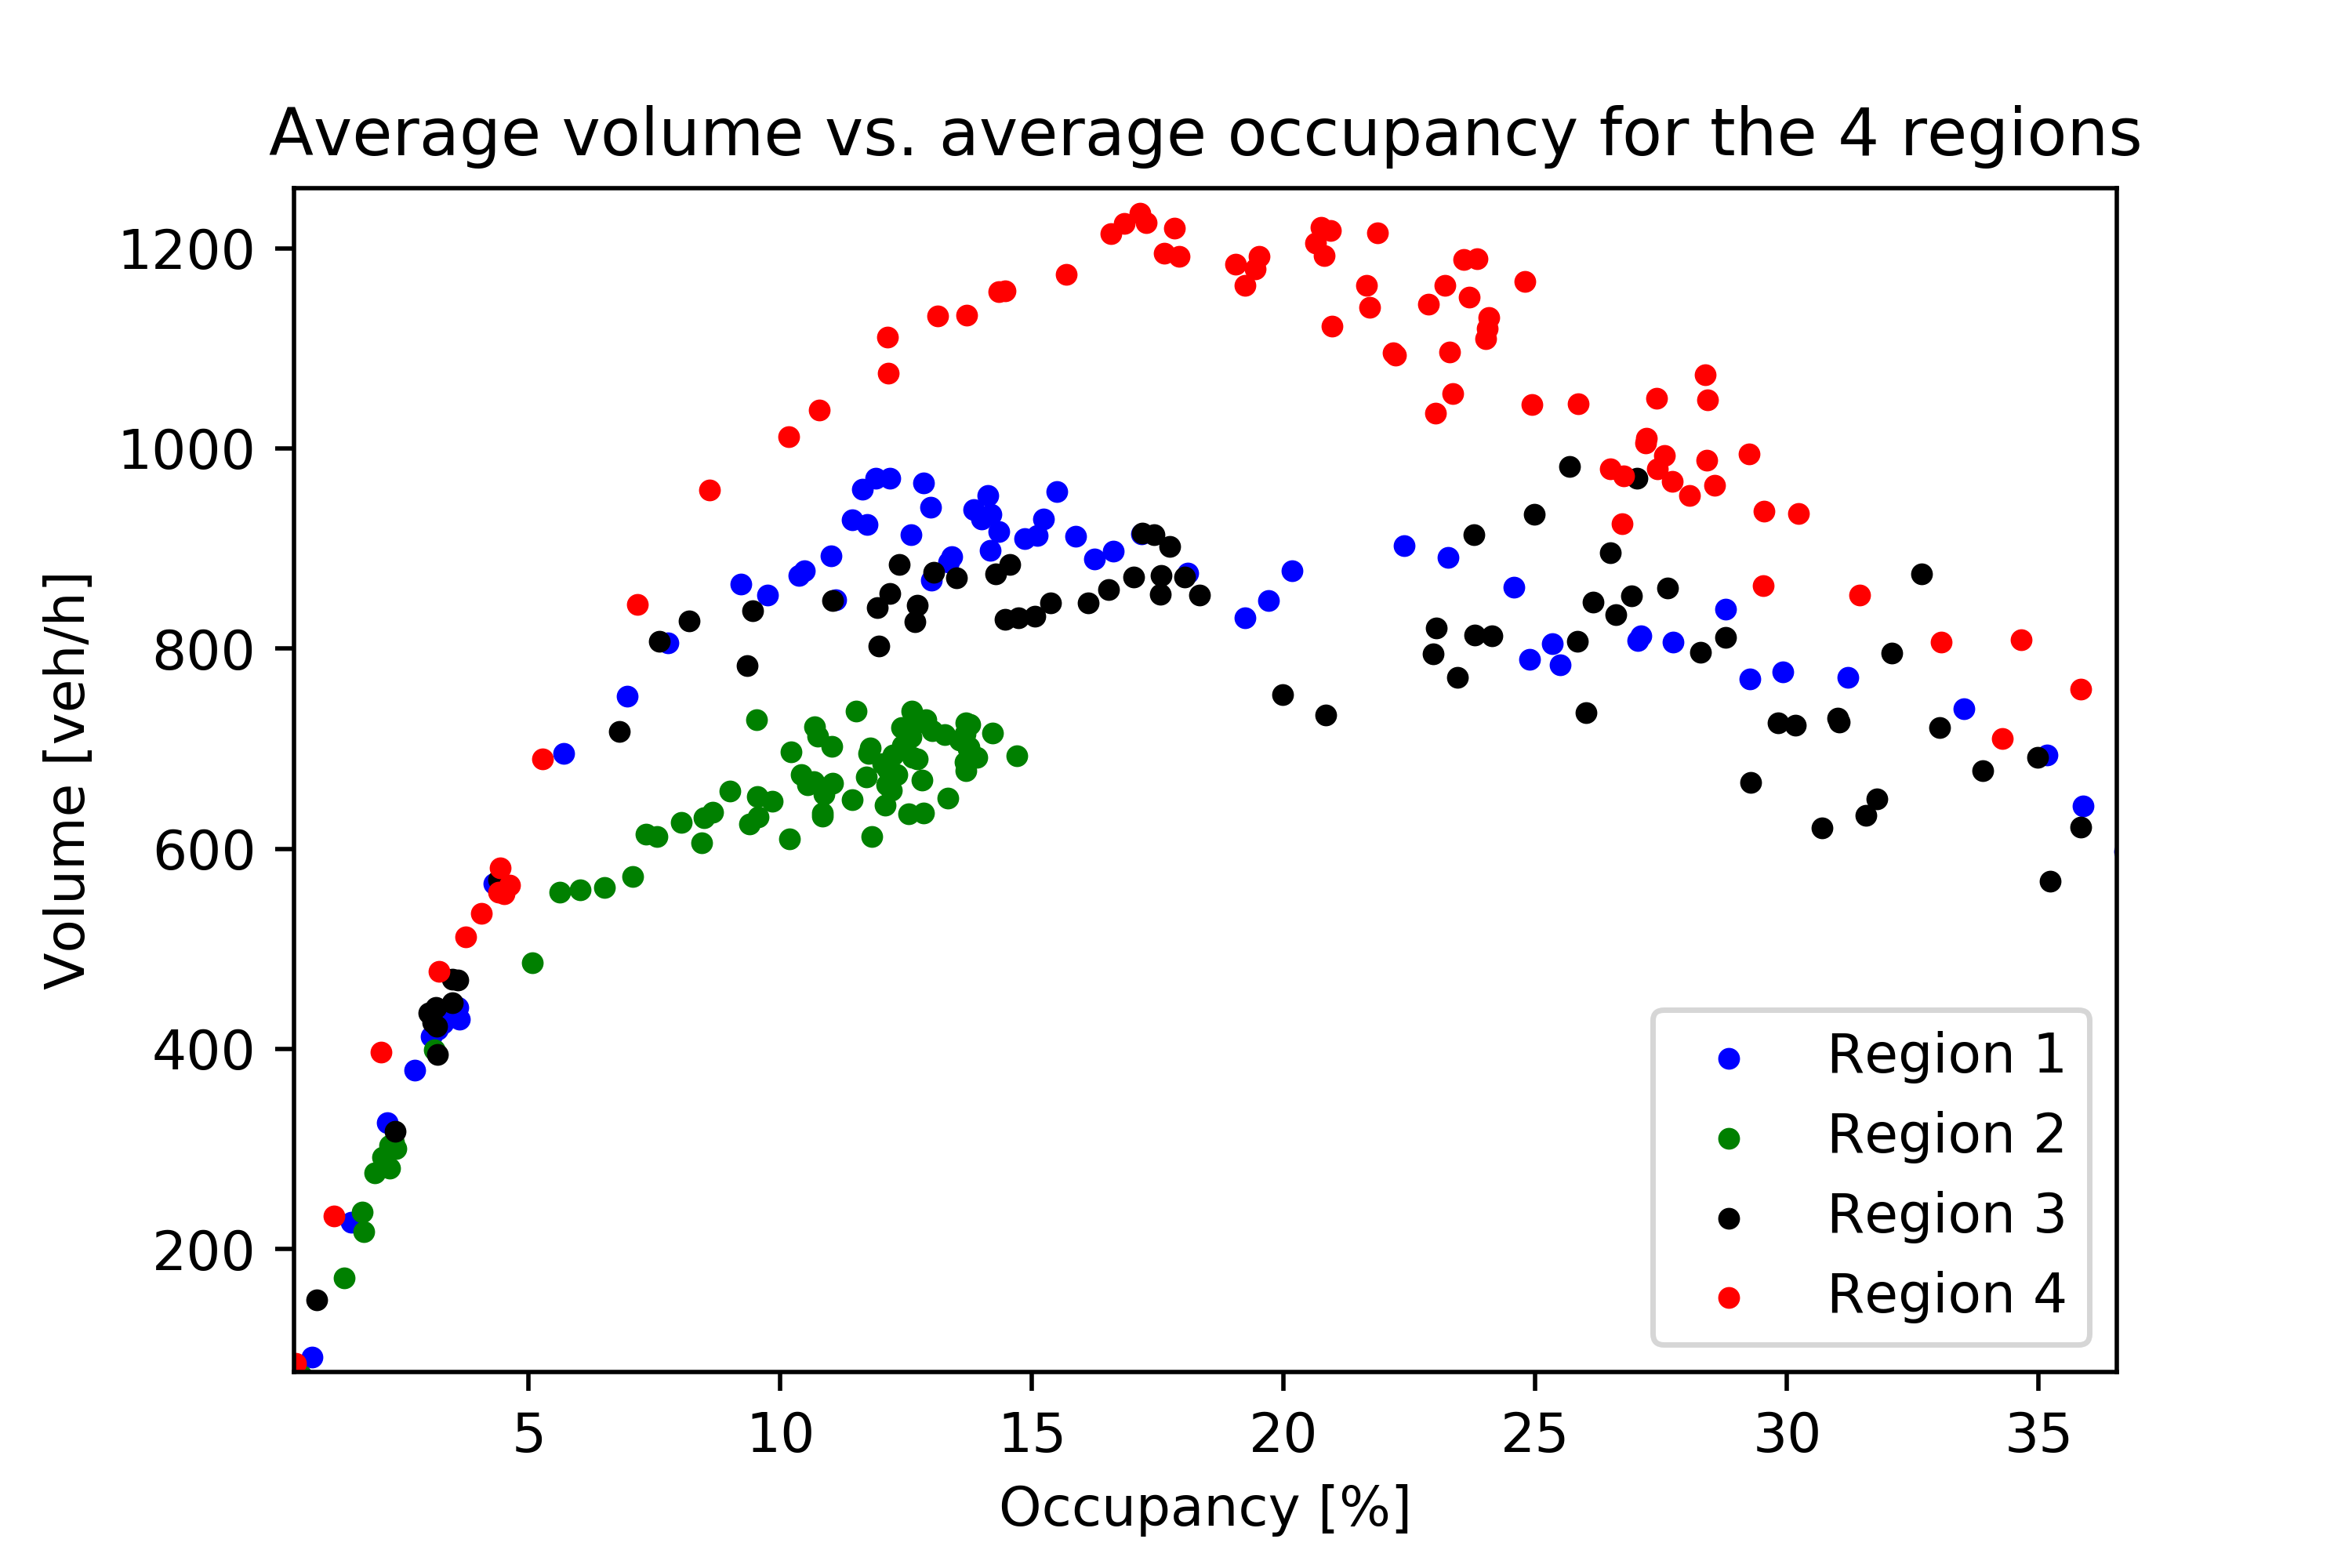
\includegraphics[width=11cm]{Images/Average volume vs. average occupancy for the 4 region.png}
        \caption{Average volume vs. average occupancy for the 4 regions}
        \label{Average volume vs. average occupancy for the 4 regions}
    \end{center}
\end{figure}


So now take a look about what's possible to see on the graphs. Common to about all the graphs in the report, analyses based on one or two paths are generally relatively poor. This is because the scatter is large and it is difficult to draw realistic and useful conclusions. It is therefore the graphs representing the different regions or the whole network that will mainly be studied because they provide much more meaningful and realistic information than one or two arbitrarily chosen paths. For example, a link might never be congested for the entire analysis and, in this case, only the first part of the MFD would be represented. In the global analysis of a region, this is less likely to happen.\\
In general for the graphs, the trend seems to be the same for the different regions. First, it is possible to distinguish a part where the network is not congested and, therefore, occupancy is low. In this phase, if the occupancy is really low, this means that the demand is also very low and therefore the average volume will also be low because there are no more vehicles to be evacuated in the network. Then, as the number of vehicles increases, the average volume will increase. However, this trend is only valid if we stay in the uncongested part of the network. Then, if the demand becomes too high, the network becomes congested, which is characterised by an increase in occupancy. From a certain occupancy value, quite similar for the different regions (around 20\% as seen in figure \ref{Average volume vs. average occupancy for the 4 regions}). Since this occupancy, the output volume will decrease with an occupancy increase due to congestion.
\smallbreak
This form of the occupancy-volume diagram is the characteristic form of the MFD (Macroscopic fundamental diagram) with 3 distinct regimes.\\ 
First, the undersaturated regime which represents the moment when the volume increases approximately linearly with occupancy.\\
Then, the efficient regime which corresponds to the maximum volume for different occupancies. This is the most interesting regime to have because it is in this case that the network is used at full capacity. It is characterised by an approximately horizontal line on the MFD.\\ 
Finally, the oversaturated regime is characterised by a decrease in volume with increasing occupancy. This is the phase to be avoided as much as possible since the network loses profitability. This is due to the fact that in congested conditions, growing queues from the downstream link block the arrivals, so it is not only the congested links that are affected but also the adjacent streets and this is how the congestion spreads, leading to a loss of volume.

\smallbreak

At the level of the different regions, it may be interesting to note that, while the shape of the MFDs is similar, the values are not necessarily so. Indeed, we can see for example on figure \ref{Average volume vs. average occupancy for the 4 regions}, which compares the different regions, that the MFDs of the different regions have different values, especially in terms of volume. Indeed, there is practically a factor of 2 between the peak values for the red region and the green one.\\
This can be explained by the fact that the average road type is not necessarily the same. The number of lanes as well as the different average speed on these roads can indeed make the output volume vary, which seems plausible in this case, but this remains a hypothesis. In our case, we know that there are different numbers of lanes in different links. Therefore, it is highly likely that this aspect plays a role in the different volumes in different regions. The assumption of a different free flow speed in uncongested areas is however not plausible. Indeed, the free flow speed is represented on the MFD by the slope of the initial uphill section. It can be seen from Figure \ref{Average volume vs. average occupancy for the 4 regions} that this slope is approximately the same for all regions and therefore it is not differences in free flow speed that fundamentally affect the output volumes.


\section{Step 3 - Density, Link speed and Mean speed}

In this step, it will be interesting to study several things.
Firstly, the density for each timestep and for each link will be calculated according to the following formula : 

\begin{equation}
       Density~k = \frac{\frac{occupancy}{100}\cdot \mu}{L+L_D}~[veh/km]
    \label{density}
\end{equation}


Then, for each timestep, the average speed of each link should be calculated using the following formula :
\begin{equation}
       Link~speed =  \frac{Volume~V}{Density~k}~[km/h]
    \label{Link speed}
\end{equation}

Finally, for each timestep, the average speed of each region is calculated. The space-mean speed of a region is expressed as :
\begin{equation}
       Mean~speed~u =  \frac{\sum V \cdot length}{\sum k \cdot length}~[km/h]
    \label{Link speed}
\end{equation}

Then, the aim is to produce scatter plots for each region with, on the one hand, the mean speed as a function of average density of the region and, on the other hand, the time-series of the region mean speed.

\bigbreak
\begin{figure}[H]
    \begin{center}
        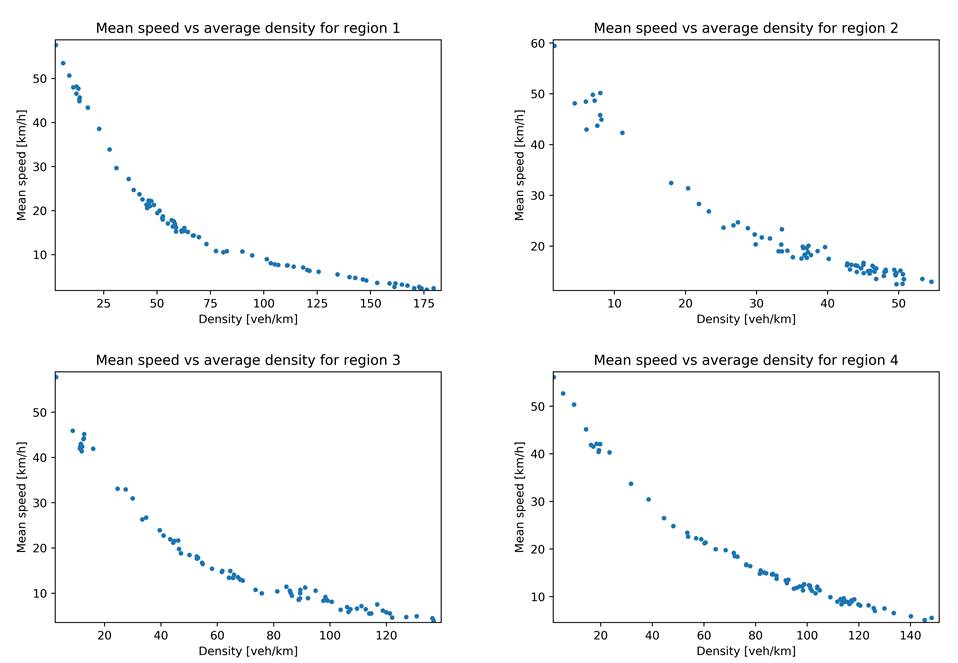
\includegraphics[width=18cm]{Images/Mean speed vs average density for the 4 regions.png}
        \caption{Mean speed vs average density for the 4 regions}
        \label{Mean speed vs average density for the 4 regions}
    \end{center}
\end{figure}

\begin{figure}[H]
    \begin{center}
        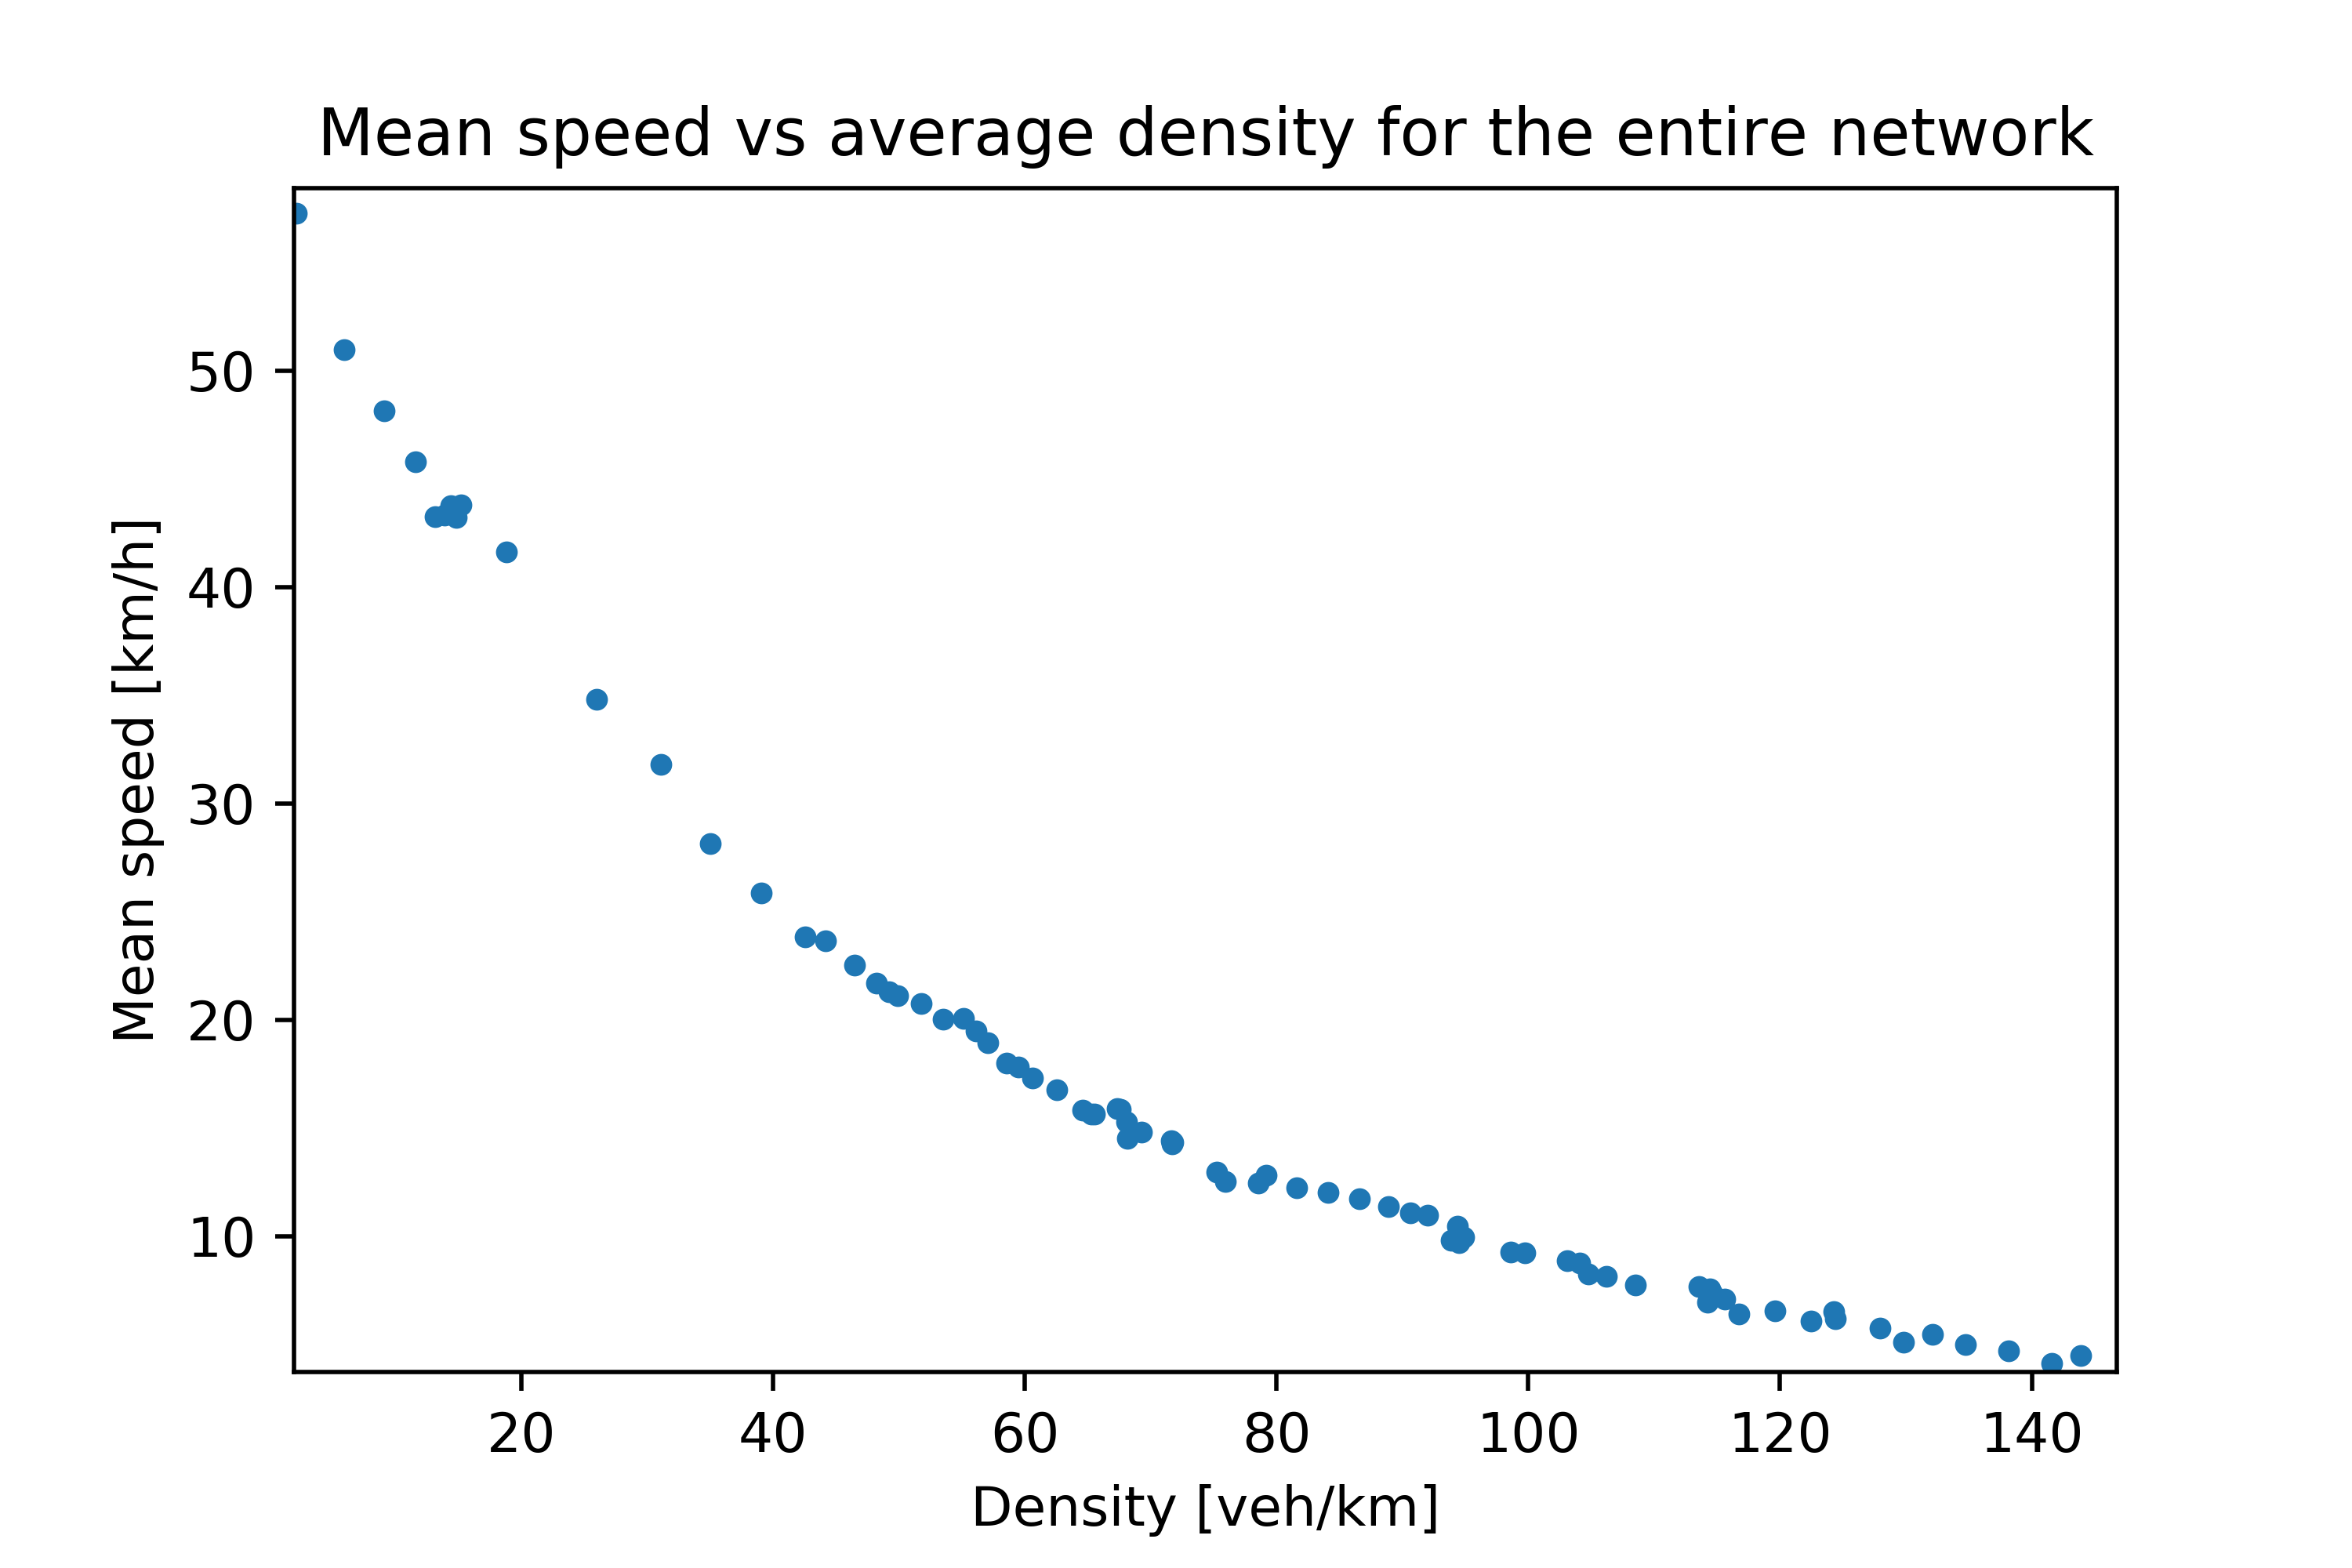
\includegraphics[width=9cm]{Images/Mean speed vs average density for the entire network.png}
        \caption{Mean speed vs average density for the entire network}
        \label{Mean speed vs average density for the entire network}
    \end{center}
\end{figure}



It is clear that for all regions, the average speed is highly dependent on density.  It is not even a linear relationship but tends more towards a hyperbolic law. This relationship is also present in the whole network. This decrease in speed with density is totally logical. Indeed, when density increases, congestion also increases, which will in fact lead to a decrease in the average speed.

\bigbreak
Then, if we look in more detail at average speeds, two main findings stand out.\\
On the one hand, for all regions, the maximum average speeds do not exceed 60 km/h. This seems totally consistent with the fact that we are in an urban network, since there are no particularly high speeds.\\
On the other hand, there is a difference between the regions in the density value of the different points. In region 2, maximum density value is much smaller than in other regions, which reflects networks that are less congested. However, the mean speed could be really low, which show that for density not so big, the traffic speed is not high, but higher than in other congested region. In other regions, it is many high density values and therefore low speeds, which shows highly congested regions at some time.
\bigbreak
In order to verify this, it is interesting to make graphs that represent the average speed as a function of time. This will allow to see the regions that are more or less congested, but also the evolution of the congestion over time.
\bigbreak
\begin{figure}[H]
    \begin{center}
        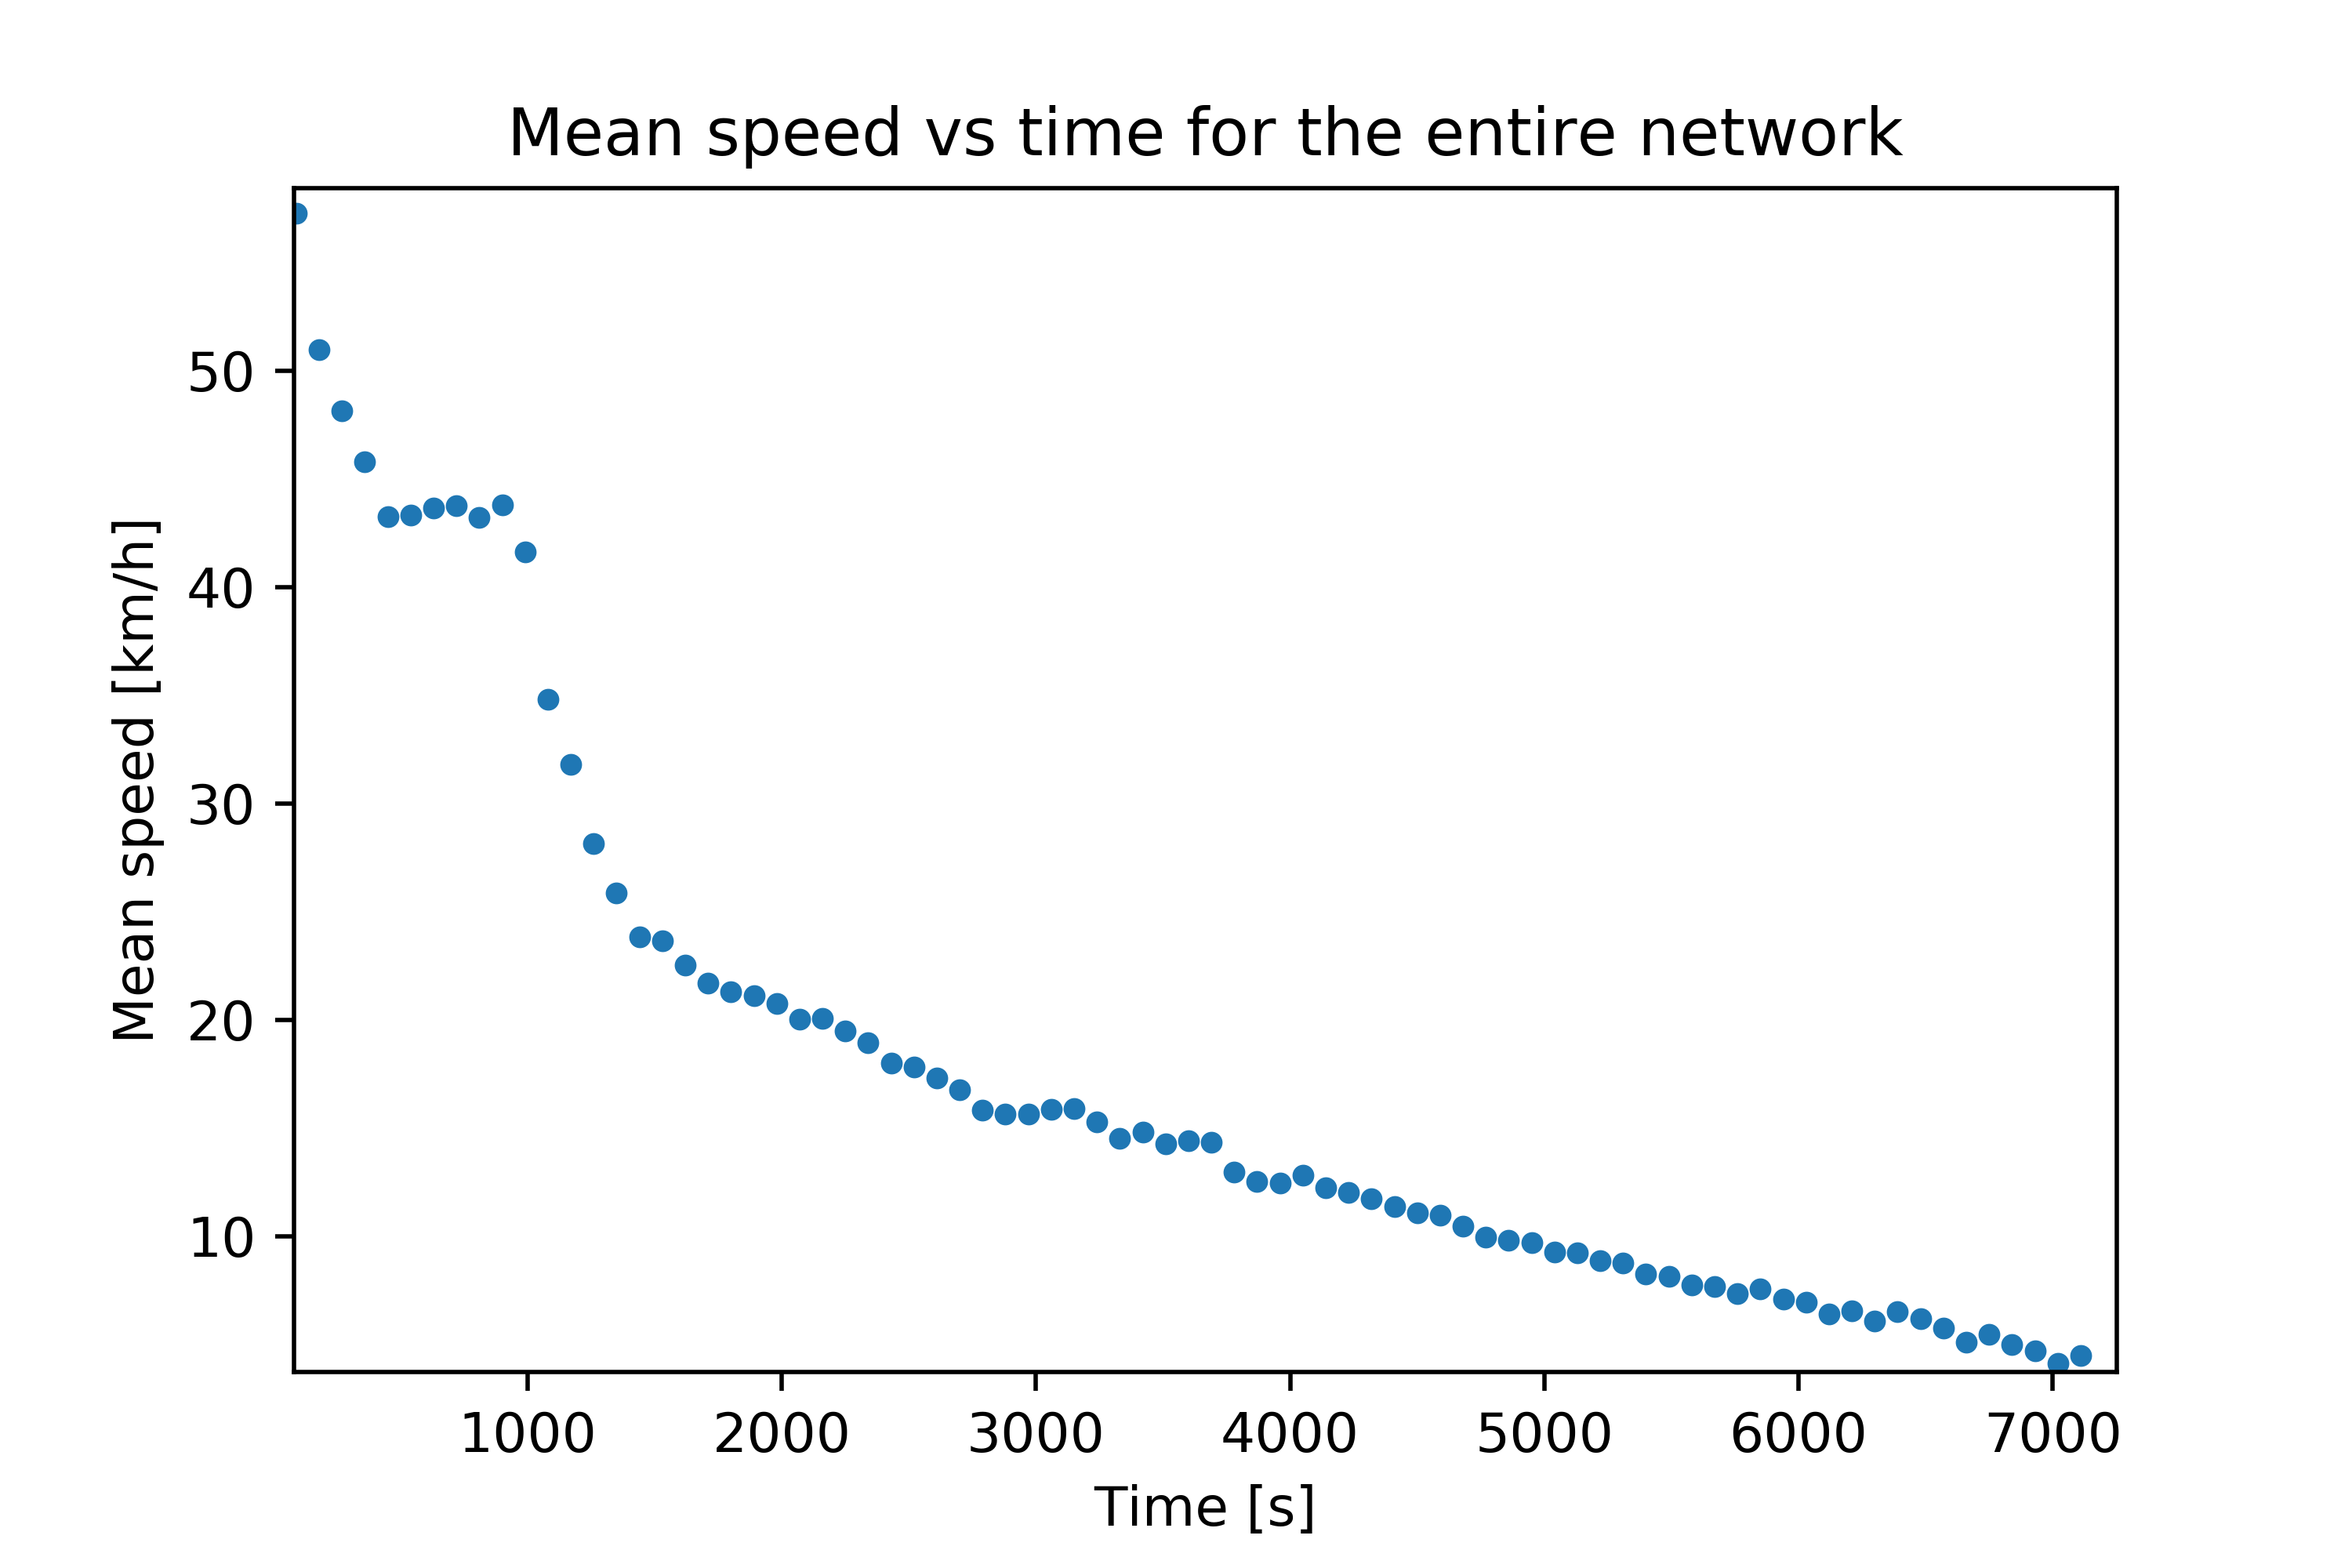
\includegraphics[width=9cm]{Images/Mean speed vs time for the entire network.png}
        \caption{Mean speed vs time for the entire network}
        \label{Mean speed vs time for the entire network}
    \end{center}
\end{figure}

\begin{figure}[H]
    \begin{center}
        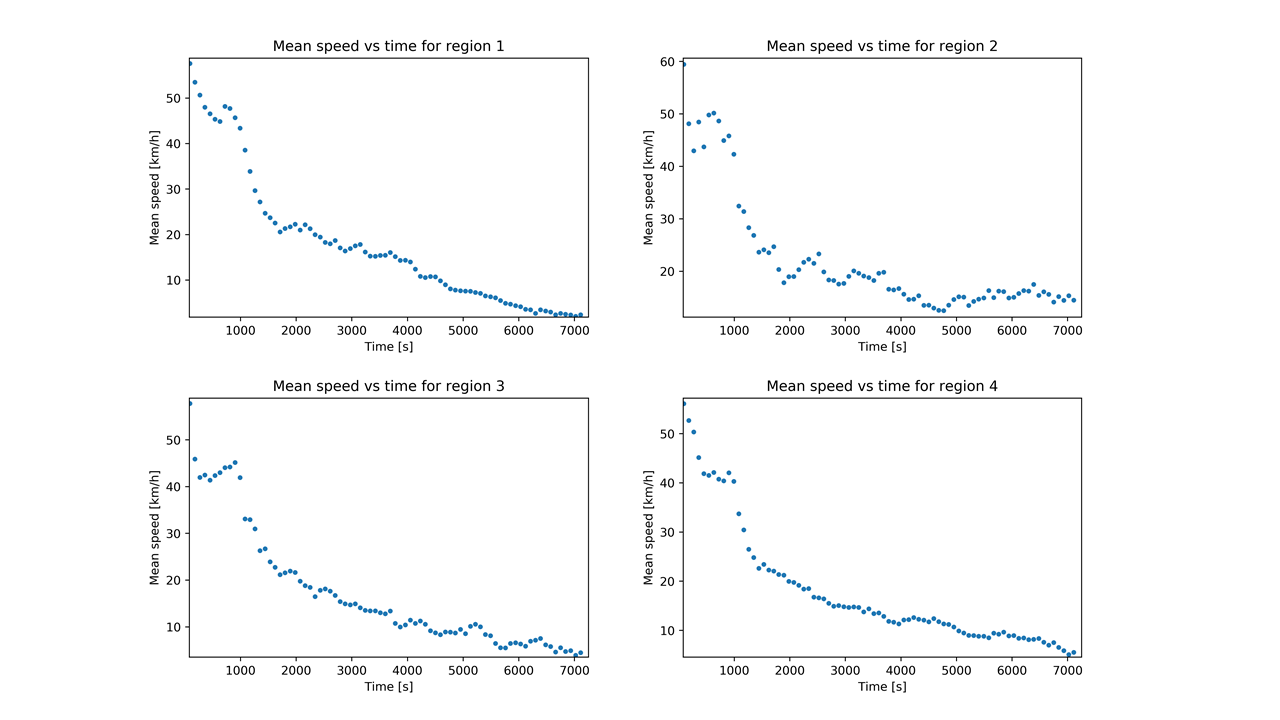
\includegraphics[width=18cm]{Images/Mean speed vs time for the 4 regions.png}
        \caption{Mean speed vs time for the 4 regions}
        \label{Mean speed vs time for the 4 regions}
    \end{center}
\end{figure}

In these graphs, two main trends can be identified.
On the one hand, slight differences are noticeable in the regions in terms of the decrease in average speed over time. As seen previously, the speed of region 2 decrease quickly but not as much as in other regions. In fact, at the end of the time of the analysis, there is no value of mean speed in region 2 less than 10 $[km/h]$, which is not the case in all other regions. This reinforces the idea seen earlier that region 2 becomes less congested over time than the other regions. The latter are however very similar to each other.\\
On the other hand, we see a common trend across all regions. The average speed decreases sharply over time, which is consistent with what we saw in question 1. Indeed, we saw an increase in network congestion over time, which coincides with the decrease in average speed.

\section{Step 4 - 
Production vs. accumulation}

It is then interesting to look at the link between production and accumulation for a random line.

The production is the volume multiplied by the length, i.e. :
\begin{equation}
       production =  volume \cdot length~[veh \cdot km/h]
    \label{production}
\end{equation}

Accumulation is the total number of vehicles in a region, and is therefore calculated as :

\begin{equation}
       accumulation =  density \cdot length~[veh]
    \label{production}
\end{equation}

First of all, for a random link, putting on the same graph the production versus the accumulation, we obtain the following graph. 
It is possible to observe that almost all the points are aligned. Thus production and accumulation are linearly dependent on this area. In fact, these points constitute the first phase of the MFD. The slope of this line corresponds to the speed of the vehicles. The study of a single link does not allow a global view of the traffic.


\begin{figure}[H]
    \begin{center}
        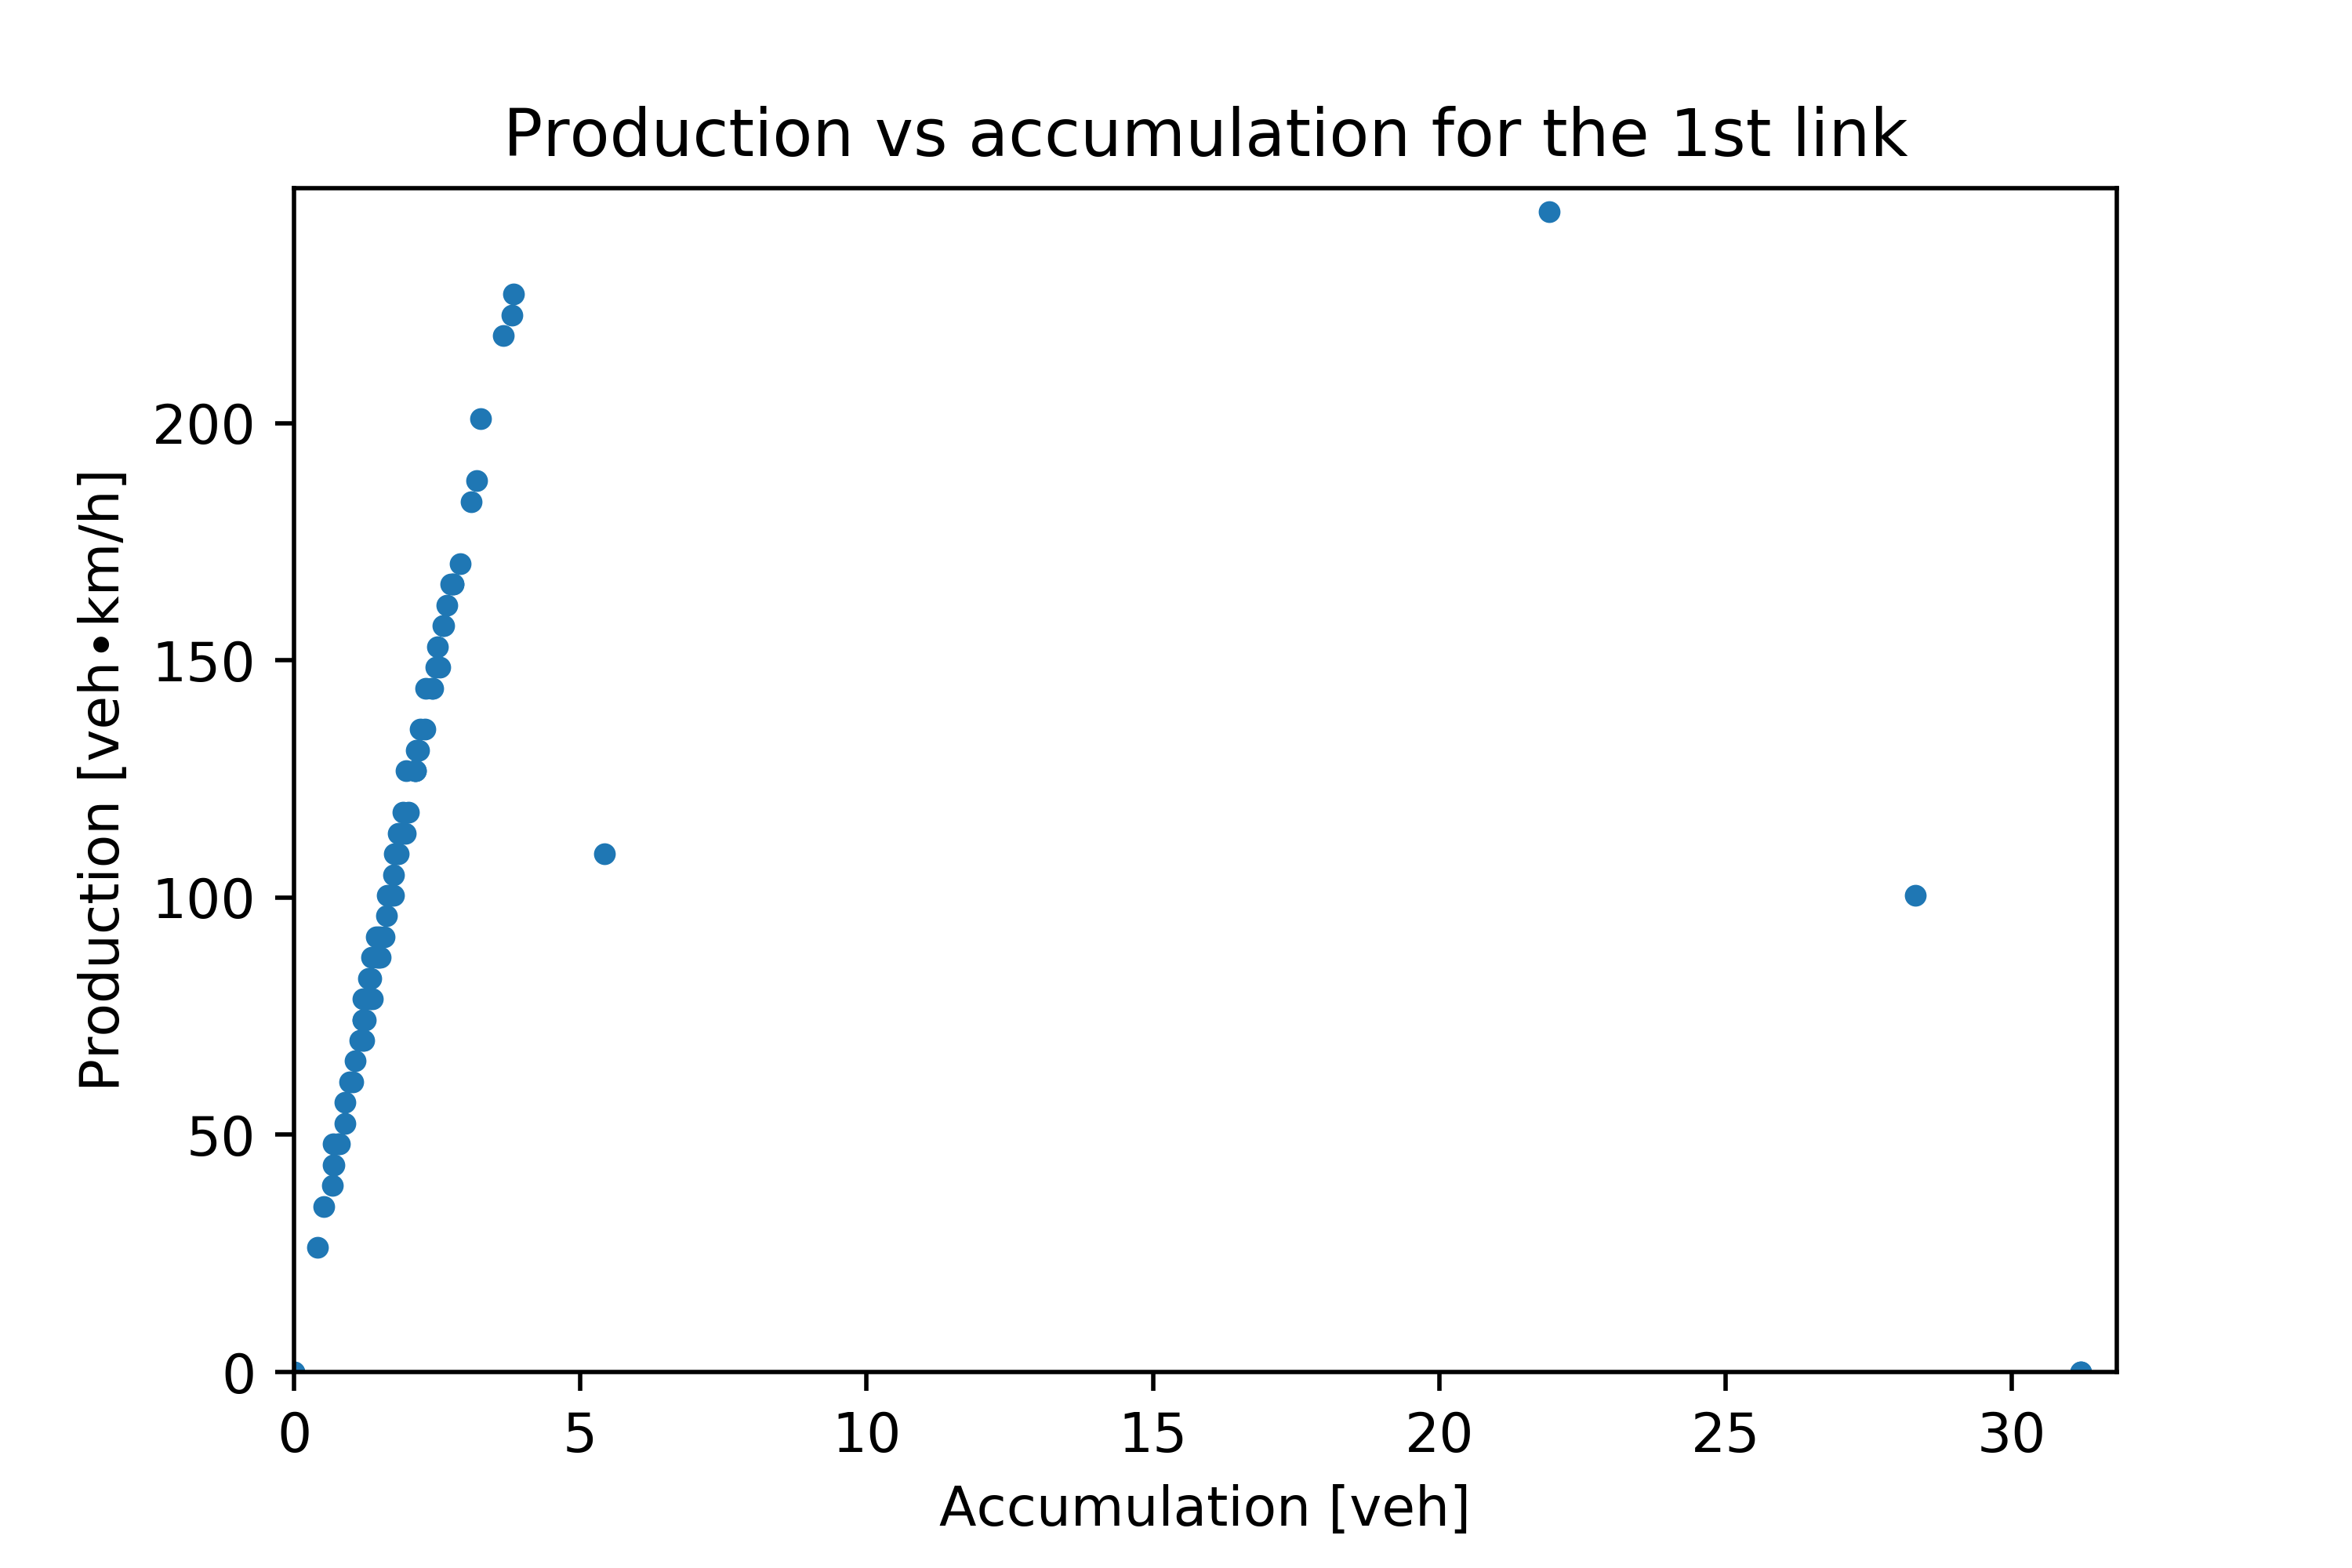
\includegraphics[width=9cm]{Images/Production vs accumulation for the 1st link.png}
        \caption{Production vs accumulation for the 1st link}
        \label{Production vs accumulation for the 1st link}
    \end{center}
\end{figure}

By producing this graph but for the sum of two links, it is therefore not easy to identify a link between production and accumulation. This is the risk in only looking at two random lines, it does not allow to have a sufficiently representative sample and depending on the values collected on these two lines, it can on the contrary make their analysis less easy. 

\begin{figure}[H]
    \begin{center}
        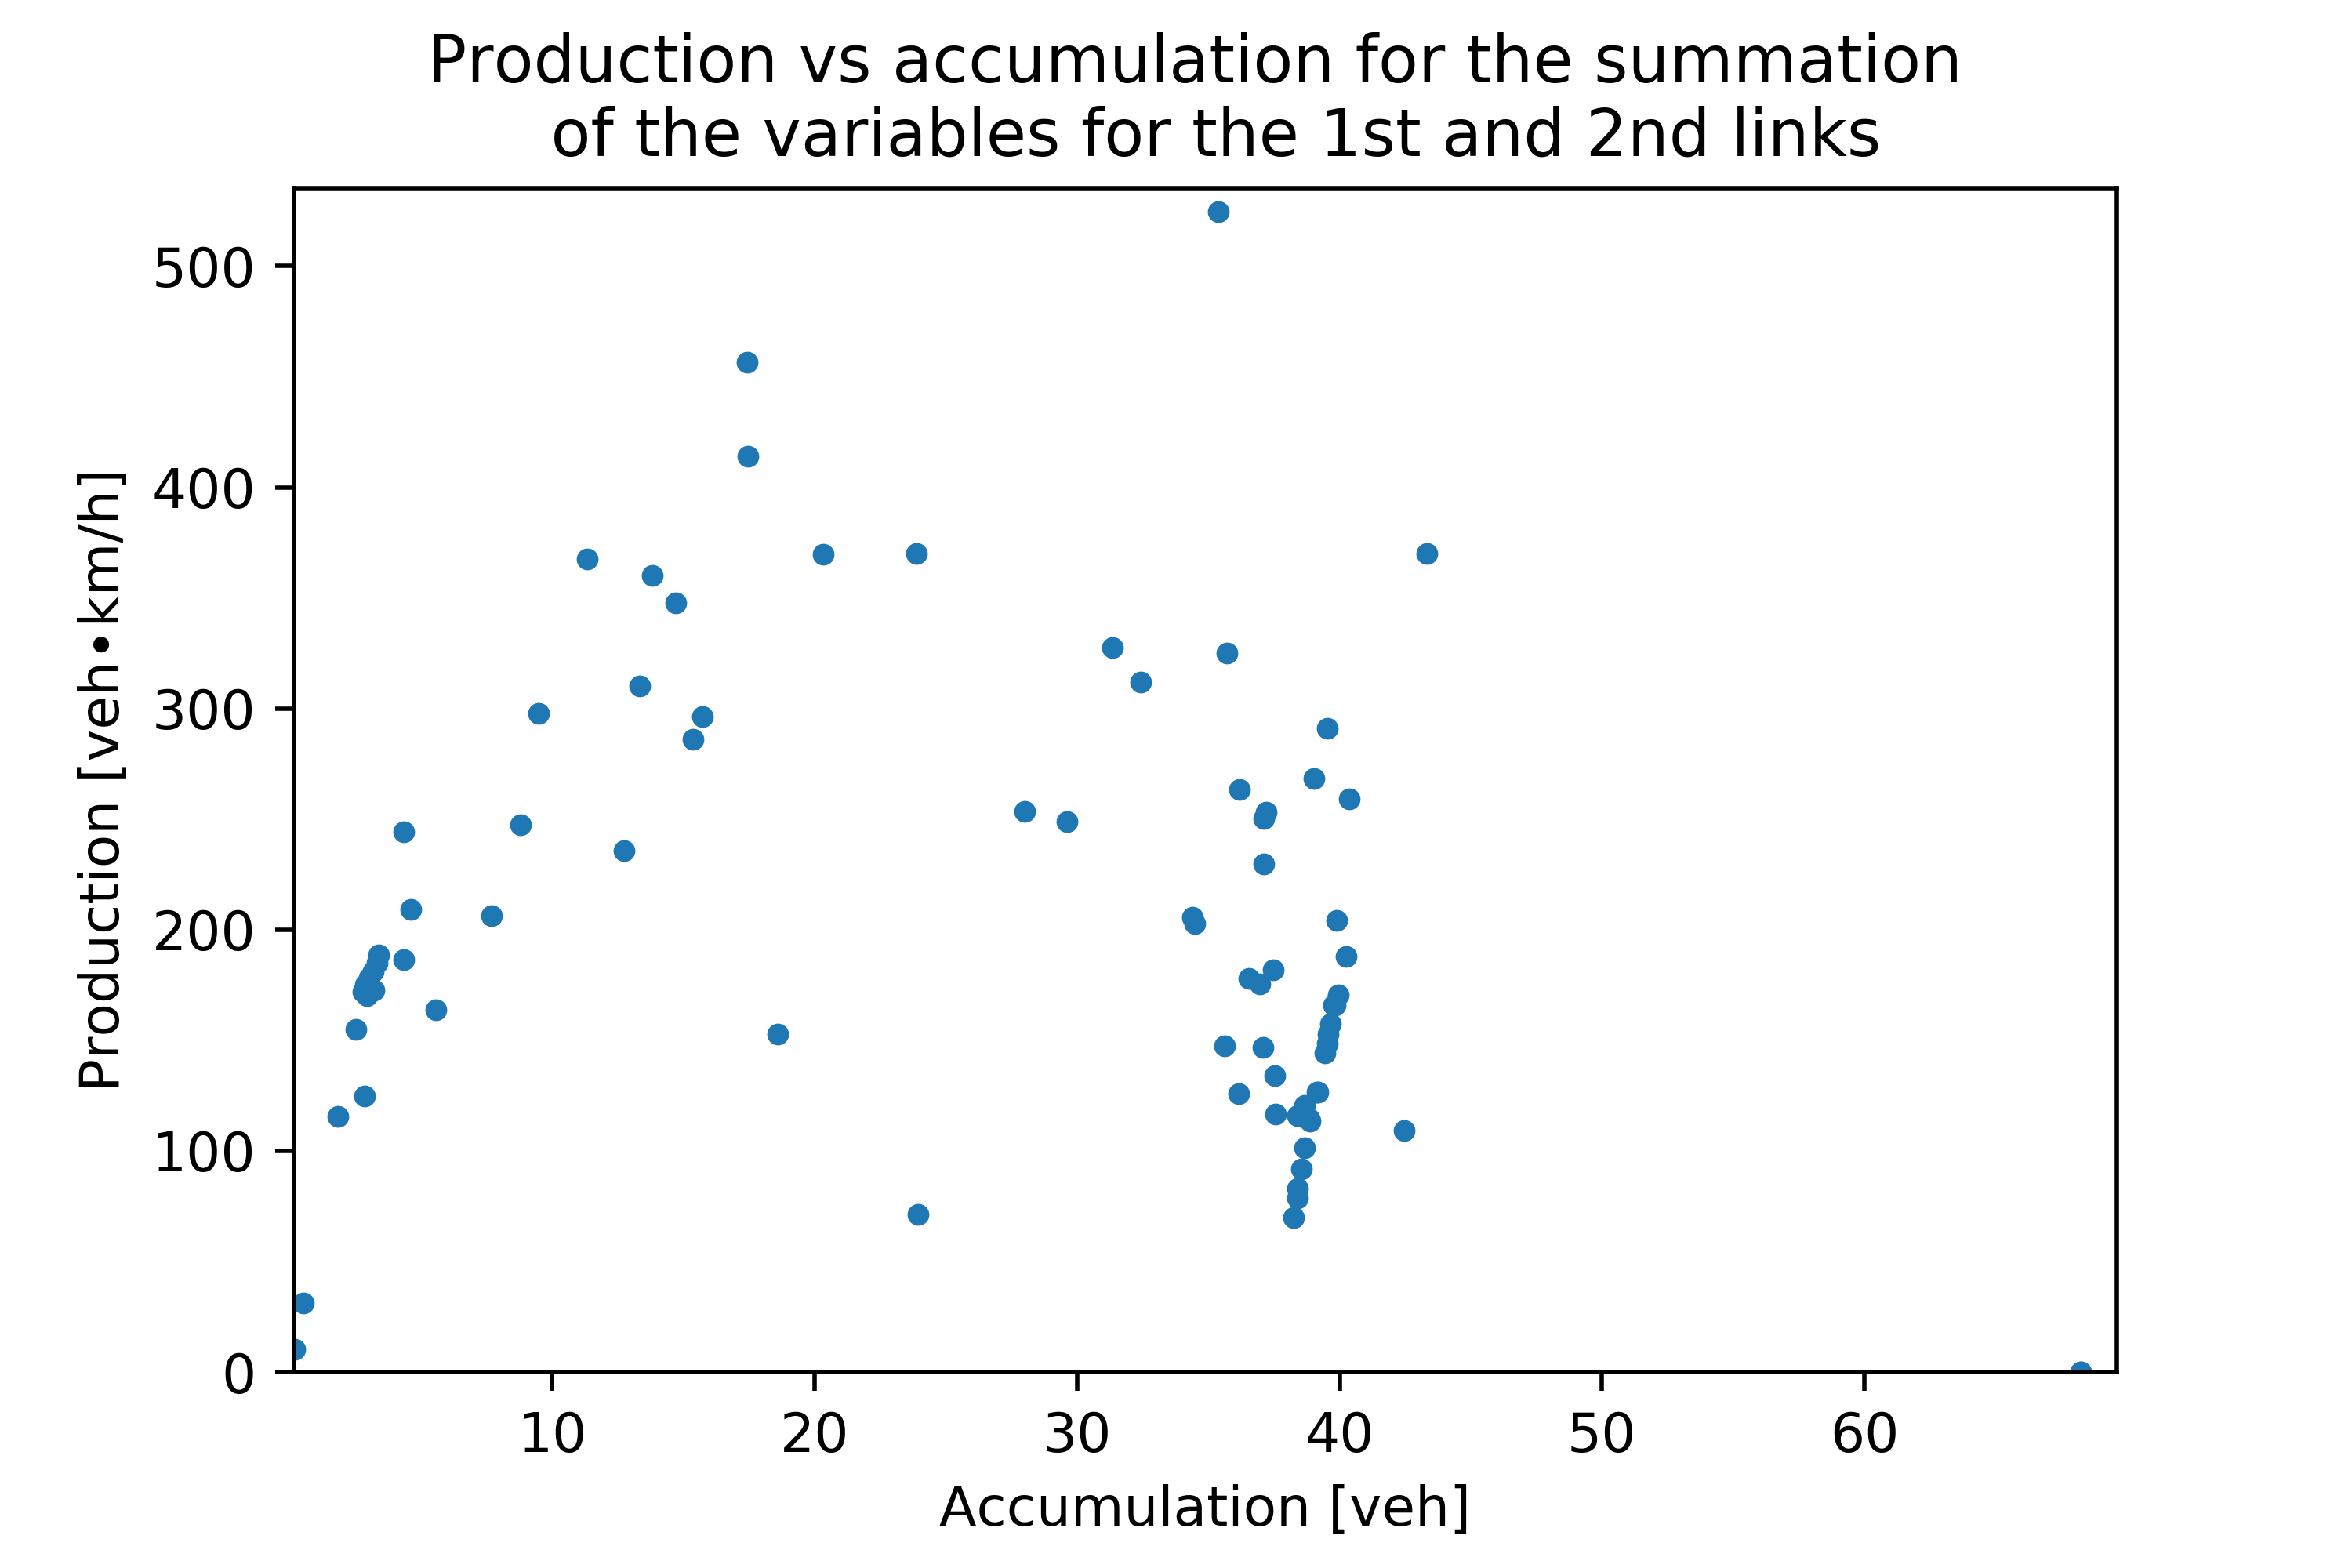
\includegraphics[width=9cm]{Images/Production vs accumulation for the summation of the variables for the 1st and 2nd links.png}
        \caption{Production vs accumulation for the summation of the variables for the 1st and 2nd links}
        \label{Production vs accumulation for the summation of the variables for the 1st and 2nd links}
    \end{center}
\end{figure}


It is therefore interesting to produce this same graph for a larger number of links. 
Processing the data for all four regions, we obtain the following MFDs:
\begin{figure}[H]
    \begin{center}
        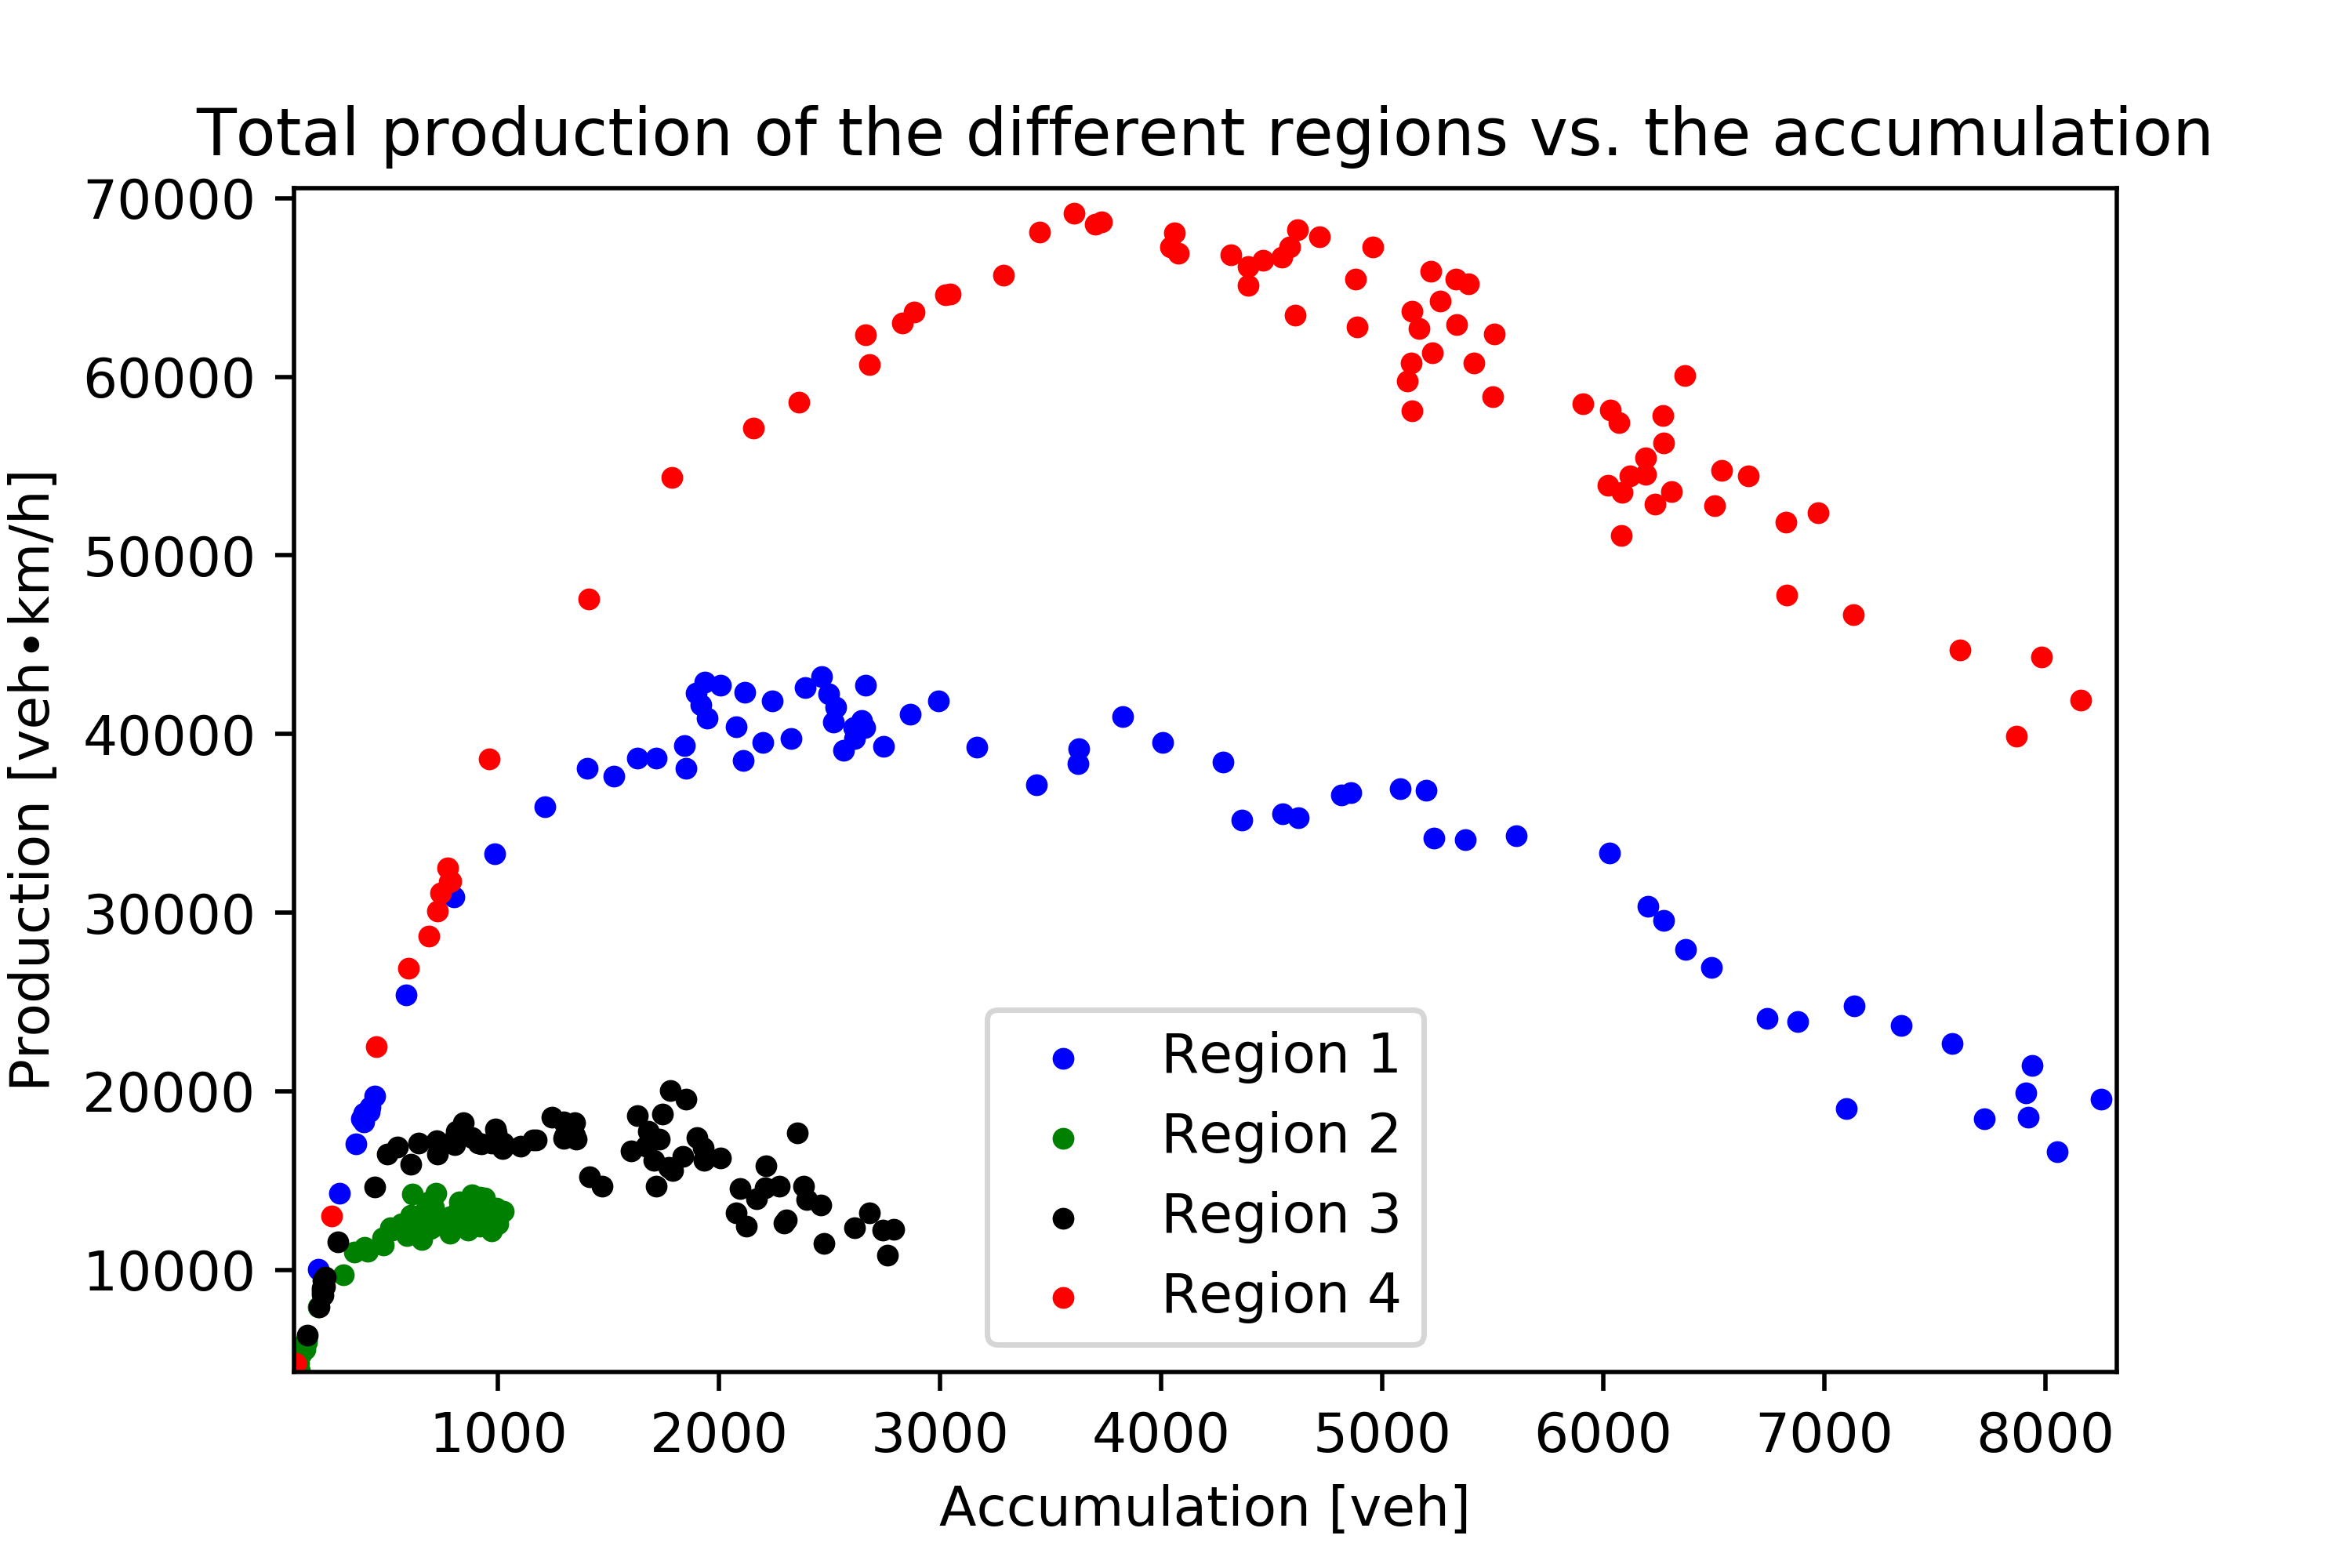
\includegraphics[width=11cm]{Images/Total production of the different regions vs. the accumulation.png}
        \caption{Total production of the different regions vs. the accumulation}
        \label{Total production of the different regions vs. the accumulation}
    \end{center}
\end{figure}

\begin{figure}[H]
    \begin{center}
        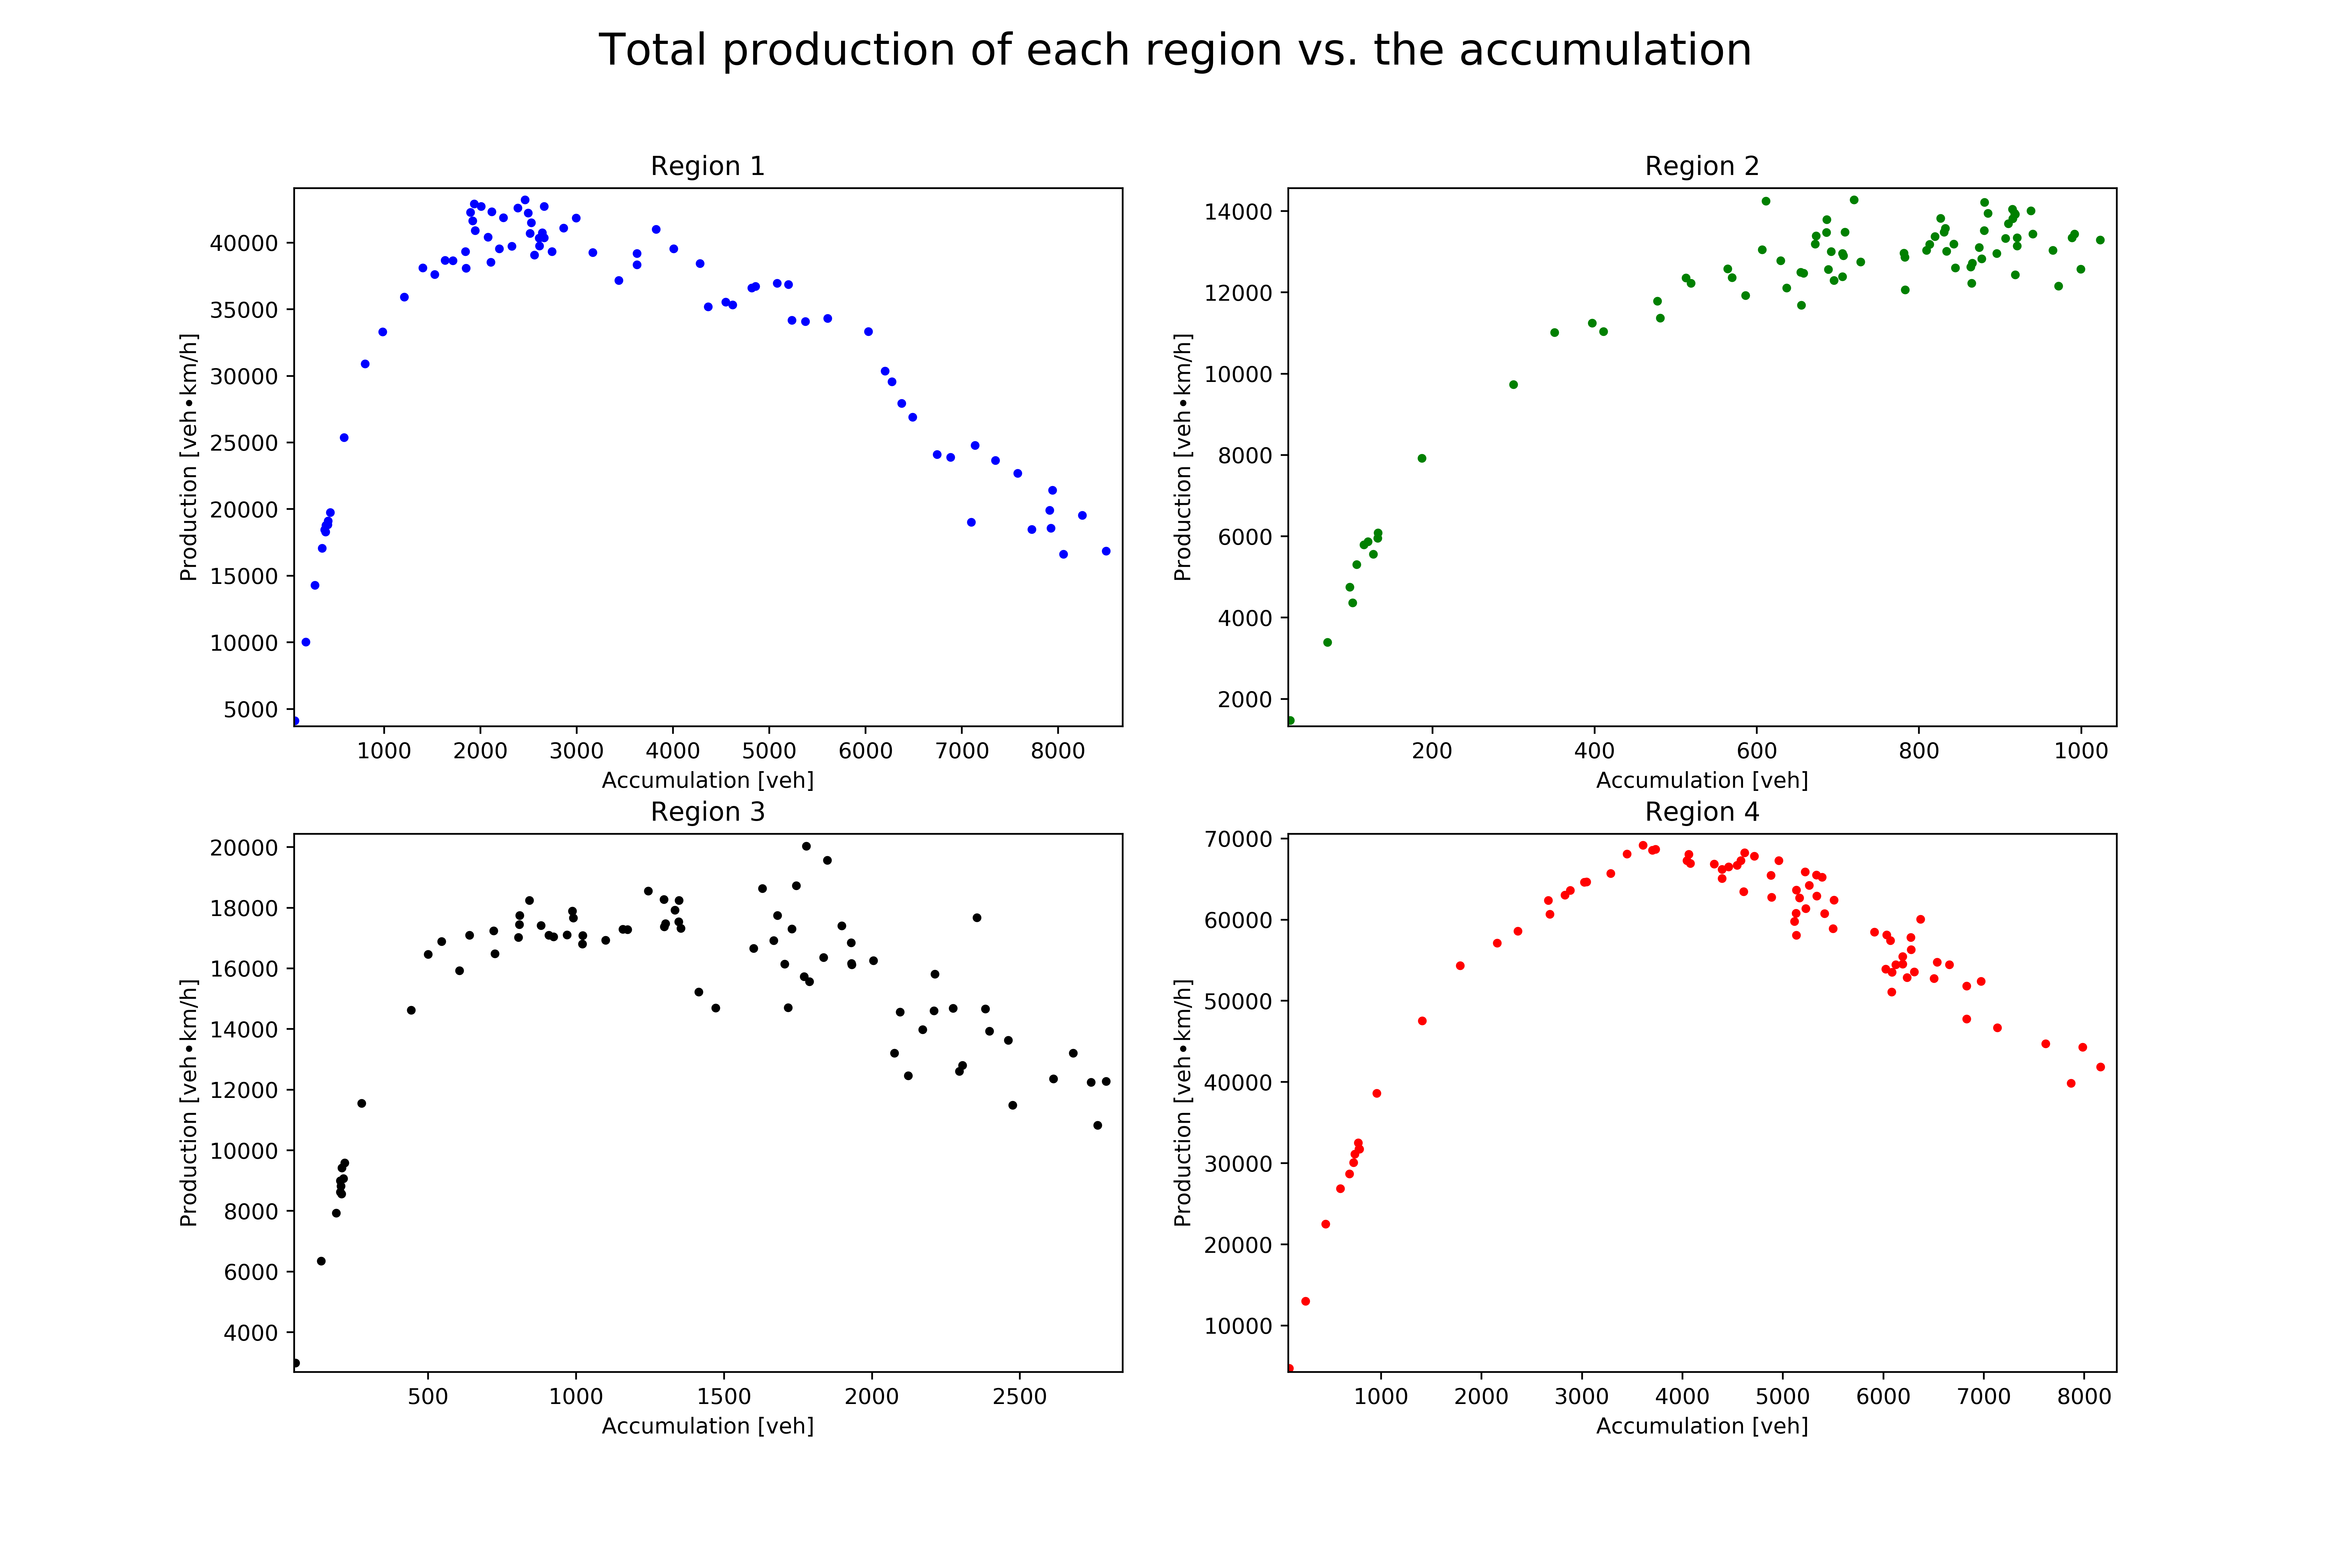
\includegraphics[width=18cm]{Images/Total production of each region separatly vs. the accumulation.png}
        \caption{Total production of each region separately vs. the accumulation}
        \label{Total production of each region separately vs. the accumulation}
    \end{center}
\end{figure}



We can observe that the shape of the curves is very similar (except for the second region), with a very high slope that leads to a very high production for a low accumulation. Then once a maximum value is reached, production decreases almost linearly with increasing accumulation.\\
It is possible to observe 3 different areas for the regions 1, 3 and 4.\\
A first one, for a low accumulation and a low production. This situation occurs when the link is only lightly occupied by vehicles. Thus, the number of vehicles is low, and the production is also low because the volume of vehicles is low.\\
Secondly, it is possible to see an area where the data appears to be much more dispersed. This could reflect different situations, where traffic is relatively dense. Indeed, the number of vehicles may be high but the traffic is relatively fluid, which corresponds to a situation where the accumulation is therefore average but the production very high. However, for the same accumulation, it is quite conceivable that the traffic is less fluid. The flow (and therefore the volume and consequently the production) is then much lower. The diversity of situations for an average accumulation thus explains the dispersion of the associated production.\\
Finally, the last identifiable zone on the graph corresponds to a high accumulation but low production. This situation reflects a zone of congestion. In fact, the density (and therefore the accumulation) is high, but the flow is not, so the associated production is low.
For the second region, the data reflects a similar slope for low accumulations, but the production becomes lower as the accumulation increases. In addition, it is interesting to note that the data stops for much lower accumulations. Thus, this region of links reflects that the density is never very high, and thus no completely congested traffic.

\smallbreak

Comparing these MFDs with the ones generated in Step 2, it can be seen that the shape of the curves is similar in every aspect. The difference between the curve in region 2 and the others is similar in all cases. Thus the link between volume and occupancy is the same as between production and accumulation. This could be expected because the production is the volume multiplied by the length, and the accumulation is calculated as the product of the density and the length. Moreover, according to the calculation of the density, the density depends linearly on the occupancy. There is therefore a relationship between the accumulation and the occupancy, as well as between the production and the volume. This justifies the similarity of the graphs.\\

However, between the graphs \ref{Average volume vs. average occupancy for the 4 regions} and \ref{Total production of the different regions vs. the accumulation}, it is possible to see that the curves seem to be distributed differently between them. Indeed, for the graph \ref{Average volume vs. average occupancy for the 4 regions} in step 2, the curves are less distant. This is due to the fact that the values are averages over time for all the channels. On the contrary for the graph of step 4, the values are the sums of the productions and accumulations for each time. The values are larger and more spaced out. Thus the spacing between the curves in step 4 is more important. 

\section{Step 5 - Strategies for reducing data}

What could also be interesting, would be to determine a method to reduce the number of data to be processed, but while keeping a result as close as possible to the data set. 
\bigbreak
To do this, it is first necessary to estimate by a curve the MFDs found in the previous step, that is to say to find a function which connects as well as possible the production with the accumulation. In view of the shape of these curves, which seem to have 2 points of inflection, approximating them by cubic functions (polynomial of degree 3) seems the most suitable. With Python, the \textit{Polyfit} function allows us to determine the coefficients of our cubic functions by using a least squares polynomial fit.
\smallbreak
\begin{figure}[H]
    \begin{center}
        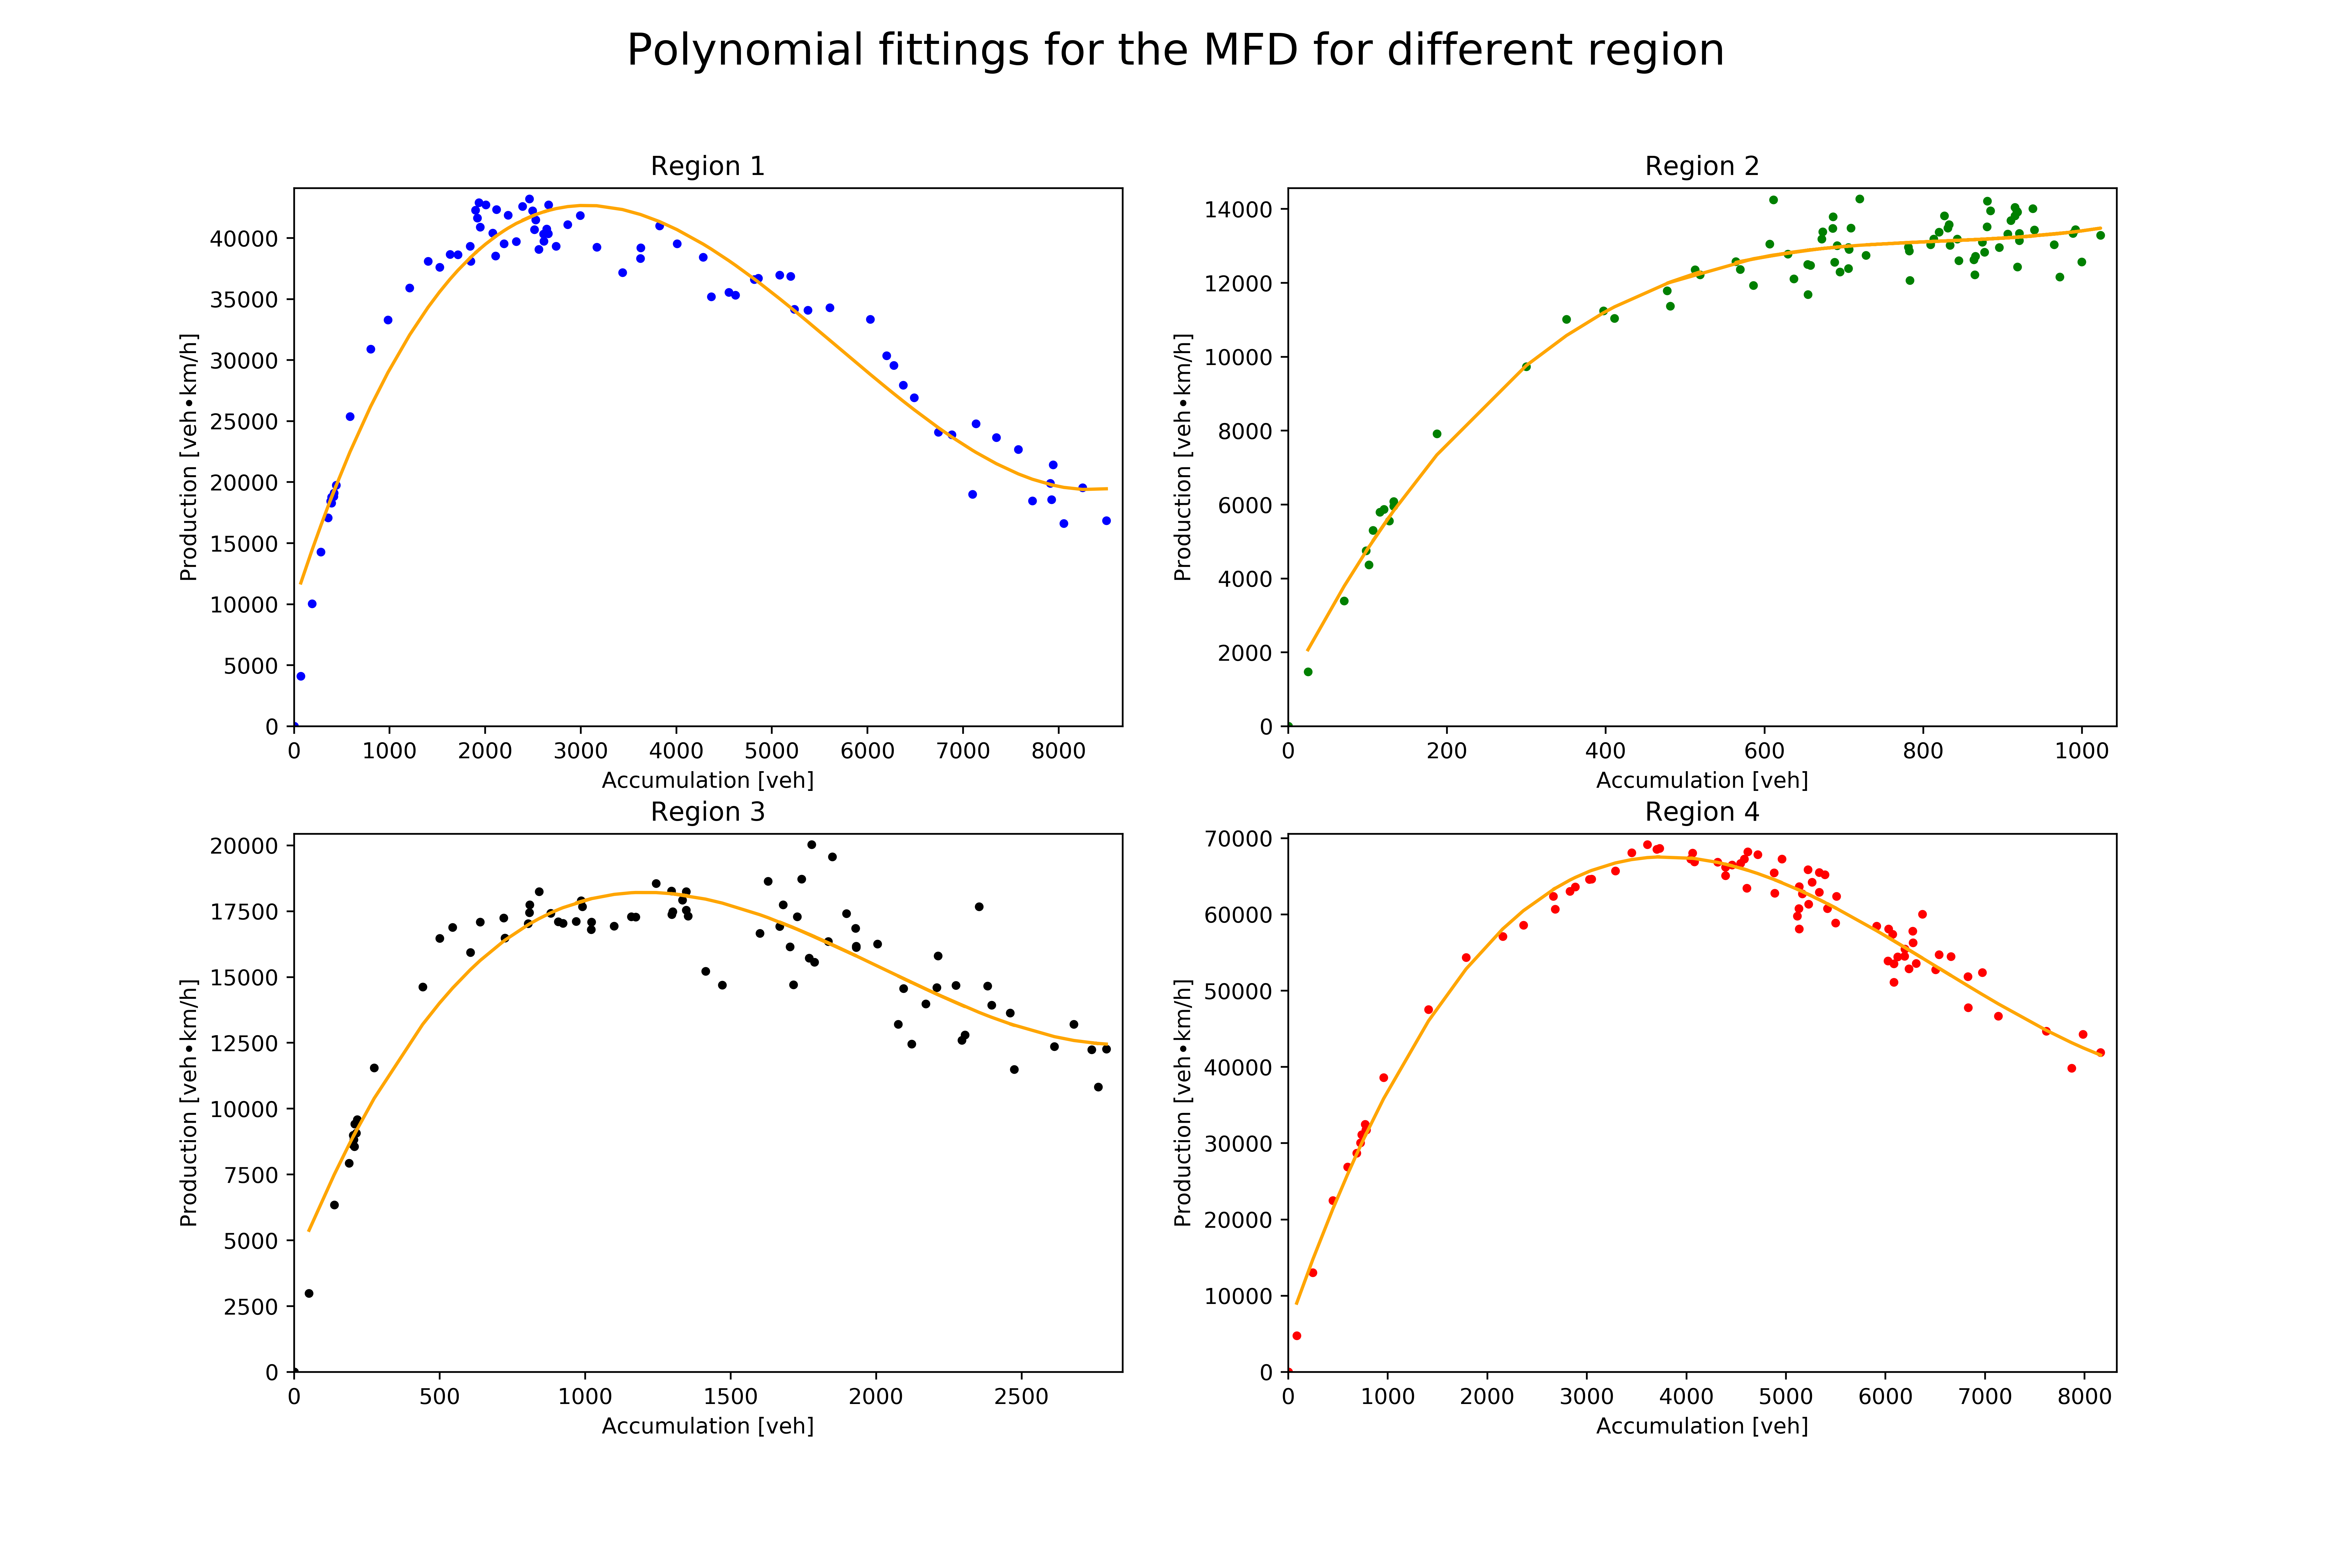
\includegraphics[width=18cm]{Images/Polynomial fittings for the MFD for different region.png}
        \caption{Polynomial fittings for the MFD for different regions}
        \label{Polynomial fittings for the MFD for different regions}
    \end{center}
\end{figure}

For each region, the equation of the curve is then :

\begin{table}[H]
\begin{center}
\begin{tabular}{|c|c|}
\hline   & curve's equation\\
\hline Region 1 & $y=3.18 \cdot 10^{-7} \cdot x^3 - 0.01\cdot x^2 + 24.31 \cdot x + 10036.6$\\
\hline Region 2 & $y=2.05  \cdot 10^{-5} \cdot x^3 - 0.05 \cdot x^2 + 42.36 \cdot x + 1051.6$\\
\hline Region 3 & $y=2.67  \cdot 10^{-6} \cdot x^3 - 0.02 \cdot x^2 + 27.44 \cdot x + 4006.5$\\
\hline Region 4 & $y=3.57  \cdot 10^{-7} \cdot x^3 - 0.01 \cdot x^2 + 37.64 \cdot x + 5891.3$\\
\hline
\end{tabular}
\caption{Equation of the MFD trend curves for each region}
\label{Equation of the MFD trend curves for each region}
\end{center}
\end{table}

It is then possible to reduce the amount of data to be processed in several ways, and to test which of these strategies results in the smallest error. Here, it is proposed to take only 50\% of the data according to different criteria.
The three strategies for data selection are:
\begin{itemize}
    \item 50 \% of the links with the highest number of lanes
    \item 50 \% of the links with the longest link length
    \item 50 \% of the links with maximum average flow
\end{itemize}

Thus, for each region, 50\% of the data must be selected according to each of the three strategies. Once this sorting of the data is done, there are 3 times 4 groups of data, that is to say 12 in total. To these data, we must also add the initial data, in order to be able to determine the errors between these data and the trend curves determined previously. In addition, this will allow a comparison for the different strategies. So, by adding the baseline data for each of the regions, there will be for each region the 3 strategies plus the baseline data. To be able to put all this data in the same graph by region, it is necessary to apply a scale factor to make it meaningful. This ratio can be calculated as follows: 

\begin{equation}
       scale~factor =  \frac{total~link~length}{selected~link~length} = \frac{\sum^{all~links} link~length}{\sum^{selected~links} link~length}
    \label{ratio}
\end{equation}

Once this factor is applied to the data, it is possible to construct graphs of production versus accumulation. 

\begin{figure}[H]
    \begin{center}
        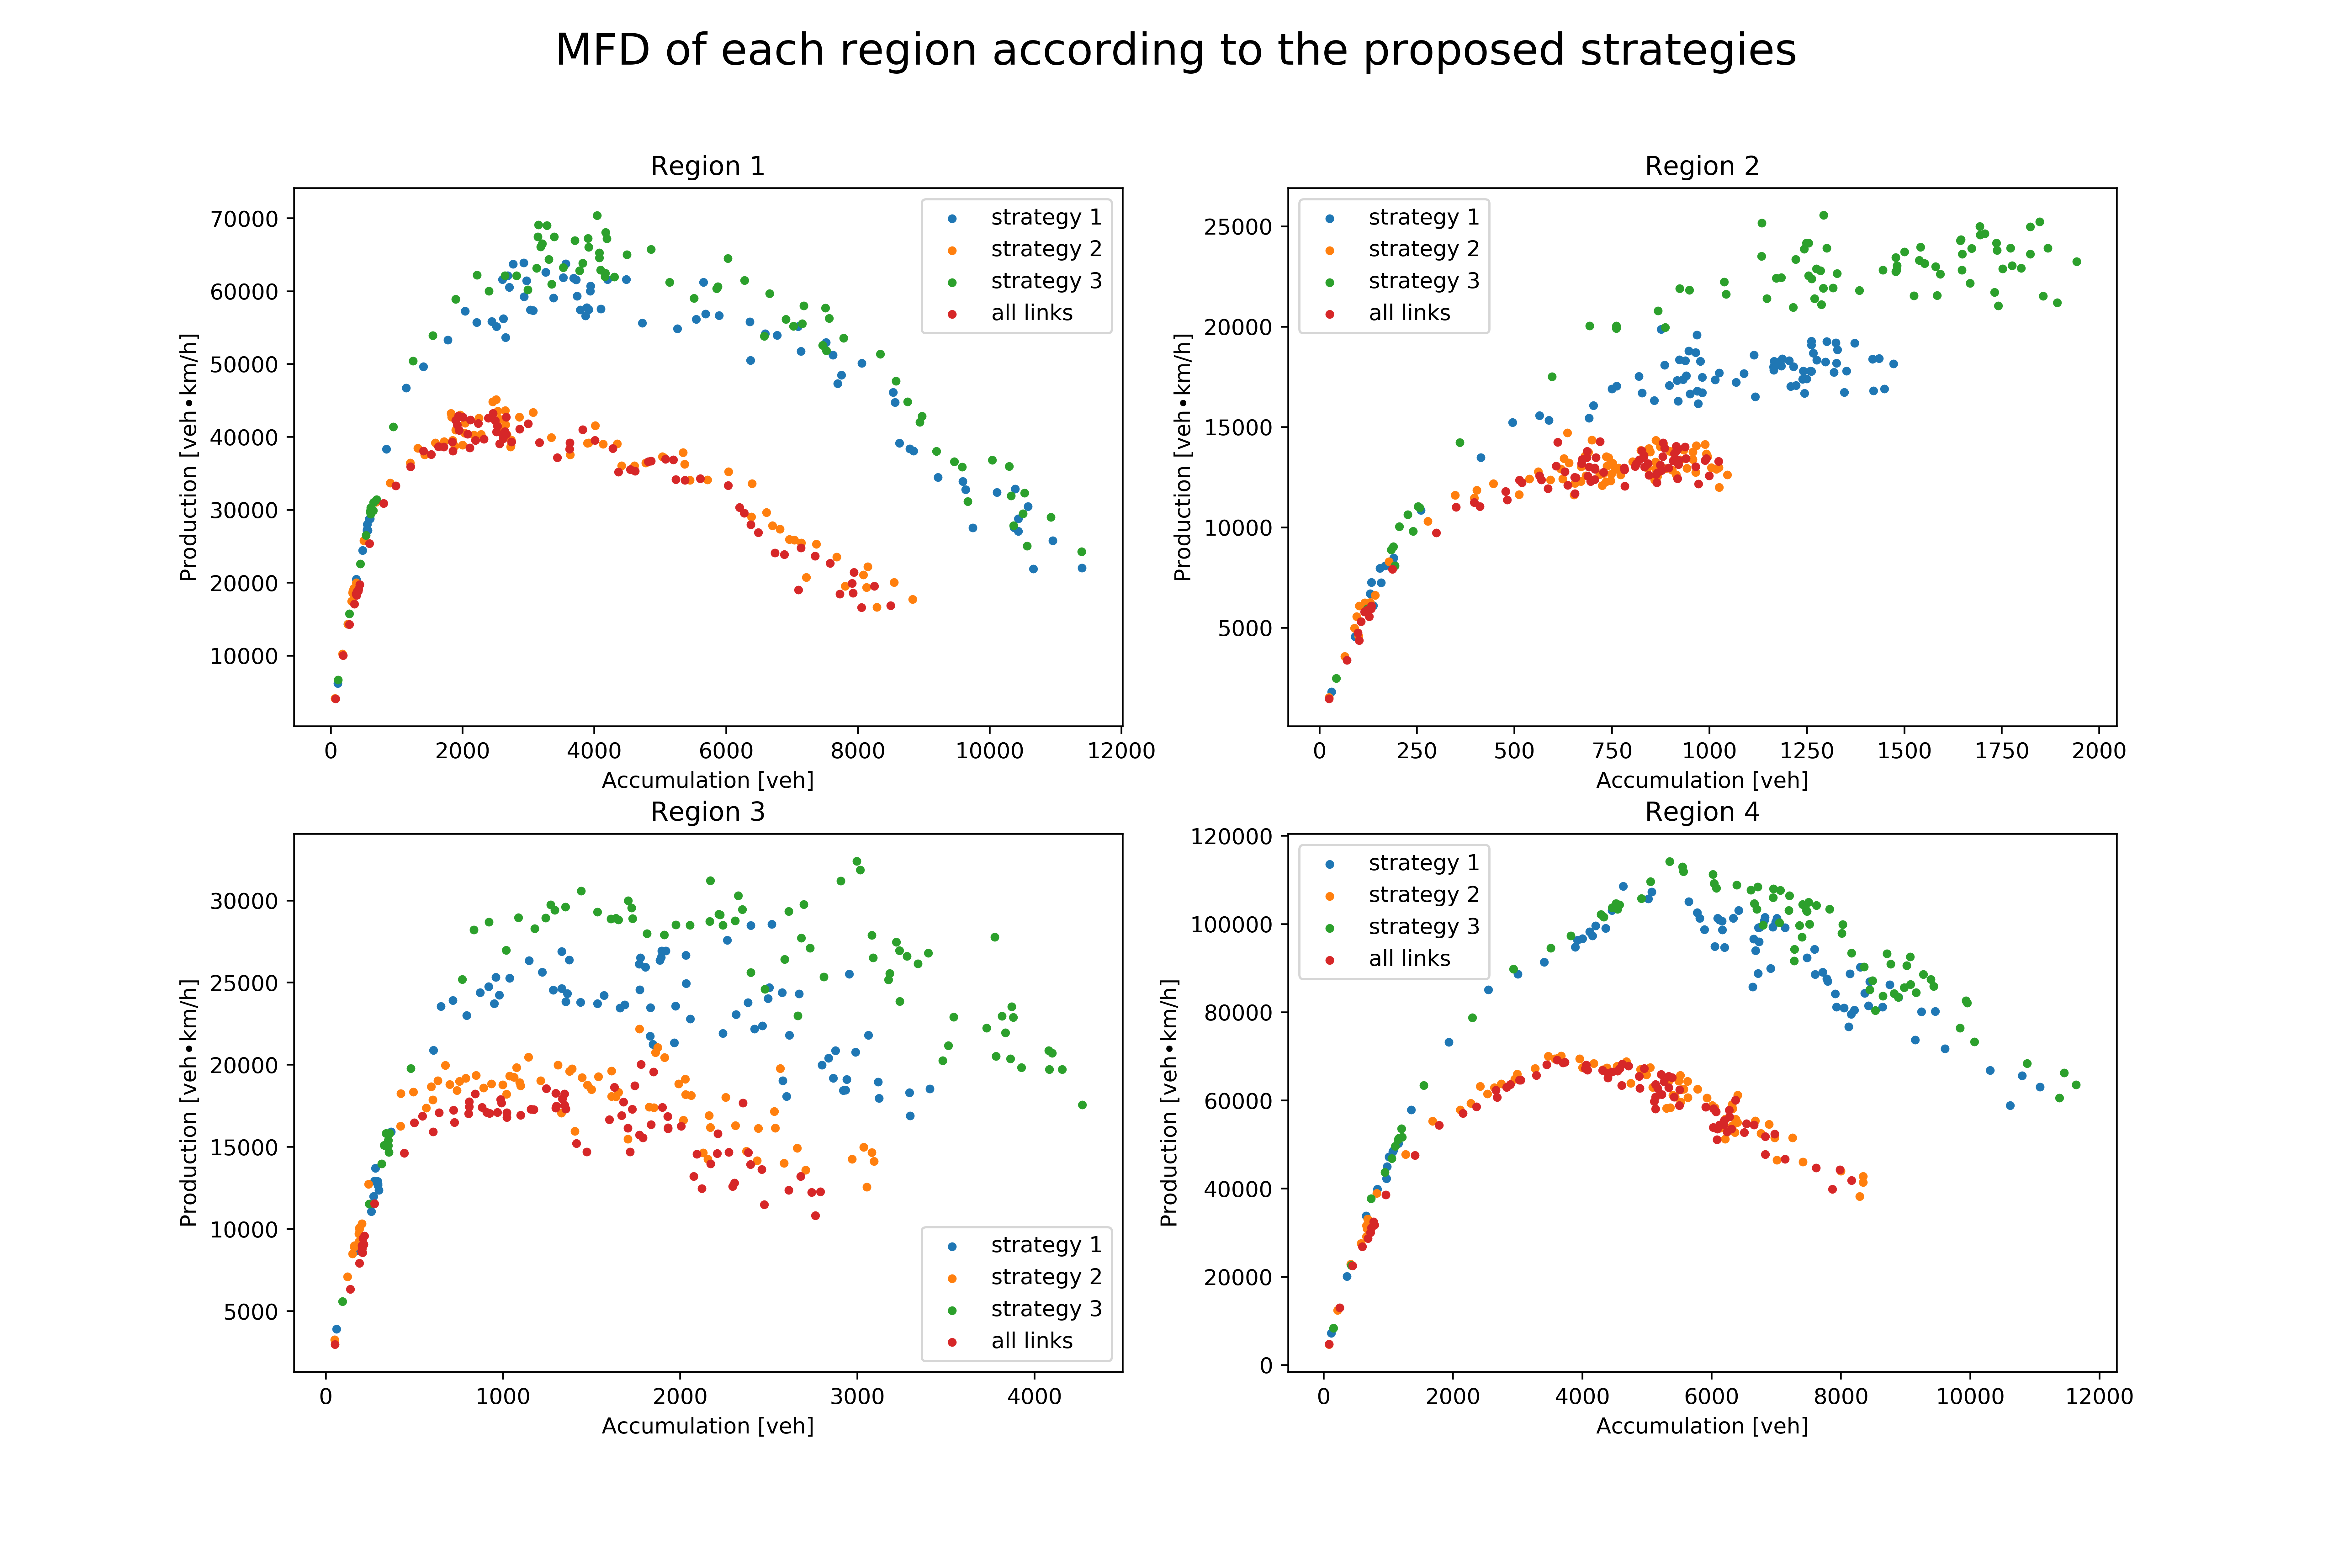
\includegraphics[width=18cm]{Images/step5plt.png}
        \caption{MFD of each region according to the proposed strategies}
        \label{MFD of each region according to the proposed strategies}
    \end{center}
\end{figure}

Looking at these graphs, it quickly becomes apparent that for all regions, the distribution of data for strategies 1 and 3 appear to be clustered and similarly for strategy 2 and the baseline data. Looking more closely, in all cases, the data for strategy 3 seems to have the highest production, then strategy 1, strategy 2 and finally the basic data.\\ Strategy 3 corresponds to the links with the largest average flows, which explains why it has the highest production because the production is linear with the flow.
\\Strategy 1 has the links with the largest number of lanes. Thus, if there are more lanes, it can be deduced that the flow is probably higher in average.  However, not all the links with the most lanes necessarily have the largest flows, so there is a small difference between the results of strategy 3 and 1.\\
Strategy 2 considers the links that have the longest length. However, since a scaling factor considering the length of the lanes has been used, it is consistent that it only increases the production more weakly than for the other lines, hence the fact of having lower values because it's approximately normalise. Thus, this strategy contains data quite close to the basic data.\\

\smallbreak
Then concerning the global aspect of the curves according to the regions, it is interesting to note that all the strategies transcribe well the regimes present in the regions. Indeed, in the regions 1, 3 and 4, the three regimes are well visible for all the strategies and for the region 2, each strategy presents only two regimes.
\smallbreak
Thus, the different strategies do not seem to have an impact on the shape of the curves, but more on the values of the data, especially because of the scaling factor.

\smallbreak
In general, the scaling factor does not seem adequate, especially for strategies 1 and 3. Indeed, it only considers the length of the links, but no normalisation parameter according to the flows or even via the number of lanes. Indeed, for example, in strategy 1, only the links with the highest number of lanes are taken into account. It is then logical, except in the under-congested condition, that the production is higher since the number of lanes is higher. It would then be necessary to consider a different scaling factor than the one used here, based only on the length of the links.\\
The general conclusion that can be drawn is based on the fact that all path selection strategies are possible, provided that a suitable scaling factor is chosen for the solution in question, which is not necessarily easy to obtain.

\bigbreak
In order to compare the results obtained with these different strategies with the network data, it is interesting to calculate and compare the fitting errors of the MFDs obtained in this step with the ones found in step 4. 

\begin{equation}
       \epsilon = \frac{1}{n} \sum^n_{i=1}\abs{\frac{E_i-P_i}{P_i}} 
    \label{error}
\end{equation}

with n the number of data, P the production for a strategy, E the production estimated with the trend curve
\bigbreak
Thus, by calculating the errors, the following results are obtained :

\begin{table}[H]
\begin{center}
\begin{tabular}{|c|c|c|c|c|}
\hline   & Strategy 1 [\%] & Strategy 2 [\%] & Strategy 3 [\%] & Baseline data [\%] \\
\hline Region 1 & 36.3 & 10.0 & 39.7 & 8.51 \\
\hline Region 2 & 17.7 & 5.27 & 27.5 & 4.14 \\
\hline Region 3 & 31.9 & 12.6 & 38.4 & 7.23 \\
\hline Region 4 & 40.0 & 5.55 & 43.7 & 4.22 \\
\hline
\end{tabular}
\caption{Fitting errors of the MFDs with strategies}
\label{Fitting errors of the MFDs with strategies}
\end{center}
\end{table}

We see that the error values confirm what we say before. In fact, error for the baseline data are logically the , just following by the second strategy. Then far away is the strategy 1 and finally the 3, totally suitable with what we see on the graphs.


\section{Step 6 - Proposed methodology for data selection}

It's now interesting to try to find the best strategy to consider less data, as it was try in question 5.
\smallbreak

The difference with Step 5 is in the scaling factor. Indeed, instead of normalising by the length of the links as it was done in step 5, it is chosen this time to consider a constant scaling factor of 2 and to try to select the 50 \% of the most representative links so that our selected data fits best with the complete base data.\\
Before proposing a strategy, it is important to look at the findings of step 5. It was first noticed that with a normalisation factor depending on the length of the links, only a selection based on this length gave satisfactory results. In fact, this observation is not accurate. In fact, it is simply necessary to look for channels that are as representative as possible in terms of flow and accumulation over the whole network, without being interested at all in the bias due to the length of the links, since this is the only bias that will be normalised due to the scaling factor. Other parameters, such as the number of lanes or the flow value of the links themselves, should not, if possible, be taken into account in the selection of the 50 \% of links studied, since this will have the effect of biasing the data, increasing the flow and accumulation values in this case.

\smallbreak
In step 6, the scaling factor does not even depend on the length of the links. In contrast to step 5, it is not possible to choose the longest links as an acceptable strategy as this will influence the data significantly.\\ 
The reflection started from the fact that, with a scaling factor of 2, it was necessary to try to find the most representative 50\% of links possible, i.e. that their average is close to the average of the whole region considered. To do this, choosing strategies based directly on the flow or on the number of lanes did not seem adequate as it could bias the result. Indeed, if we decide, for example, to choose only the links with a certain number of lanes, we will necessarily impact the production and accumulation values. The last criterion we could use to choose our strategies was a criterion based on the length of the links. However, as explained above, it is not a question of taking only the longest links since the scale factor does not depend on the length of the links, but rather of trying to take the most representative values possible.
\smallbreak
Initially, it seems interesting to concentrate on the average values and thus neglect the tails of the distribution. Depending on the practical distribution, this strategy can be very correct, but also very wrong if the distribution tails have a non-negligible impact. It was therefore decided to consider all links between 25\% and 75\% of the link length. Extremely short links are therefore neglected, as well as the longest ones. The results found are presented below :

\begin{figure}[H]
    \begin{center}
        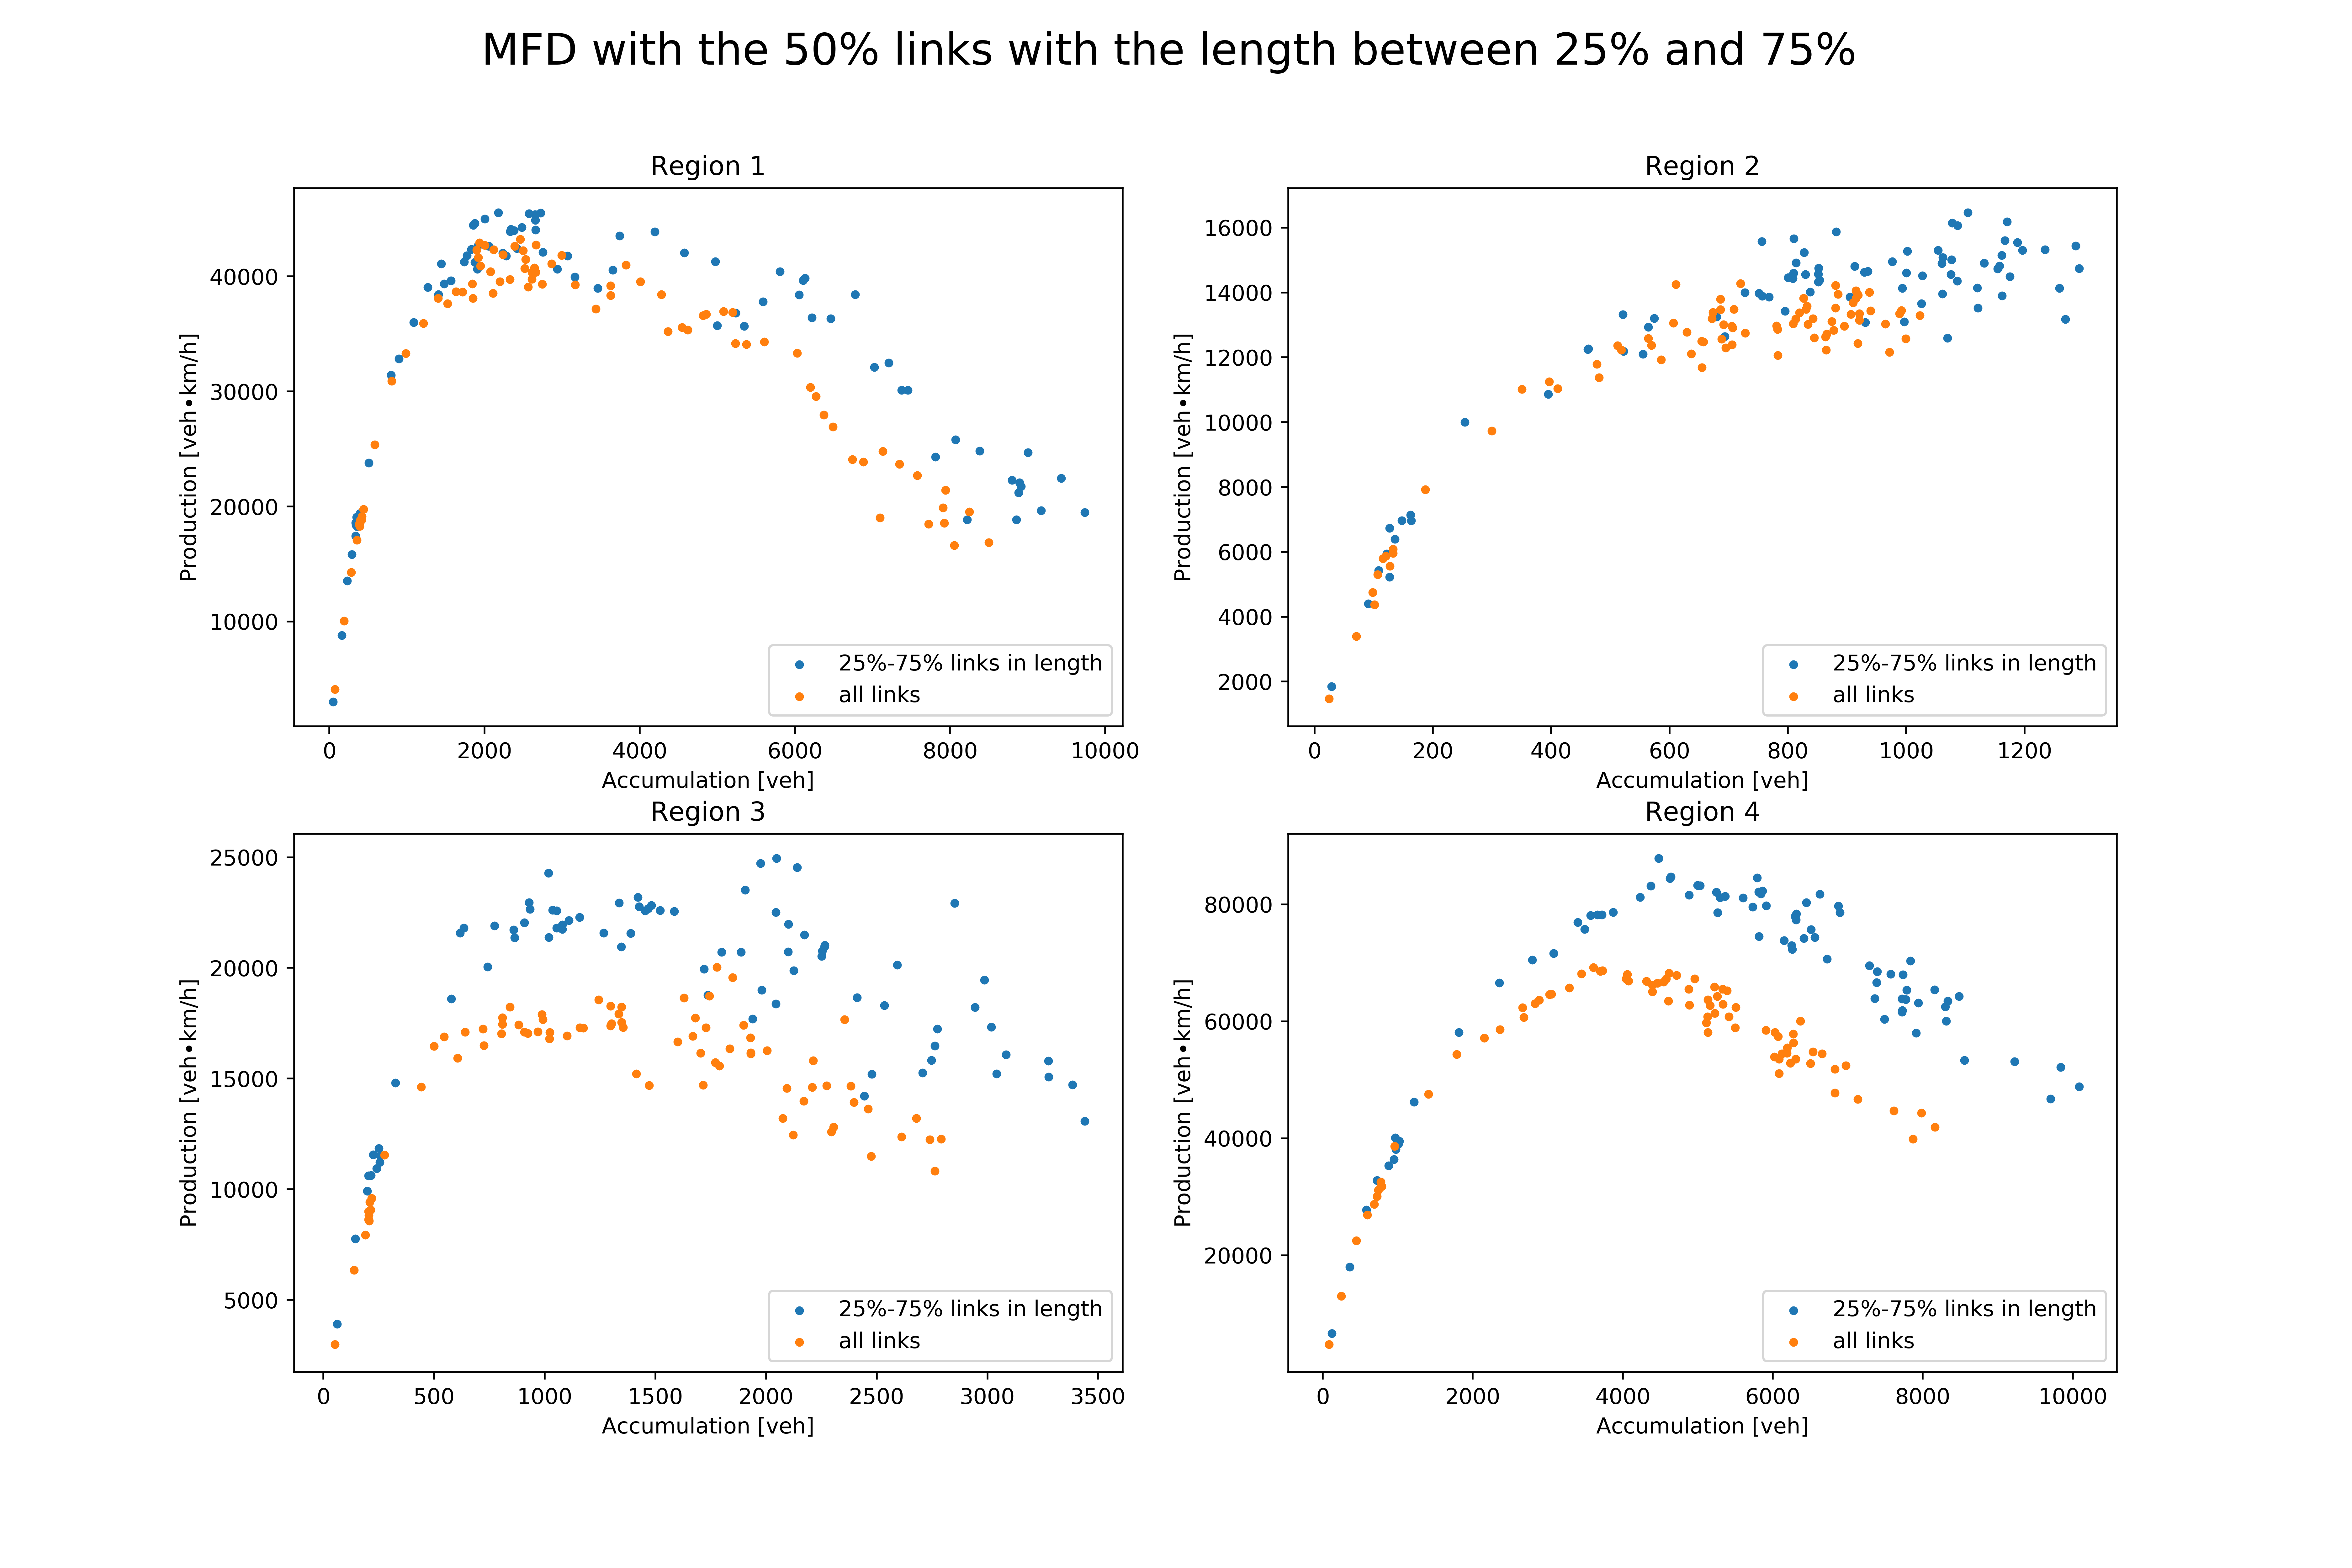
\includegraphics[width=18cm]{Images/step6_25_75.png}
        \caption{MFD with the 50\% links with the length between 25\% and 75\%}
        \label{MFD with the 50\% links with the length between 25\% and 75\%}
    \end{center}
\end{figure}

\bigbreak

We can see that the results are quite good overall, although far from perfect. For regions 1 and 2, the values seem to be good, although we start to see some bias in region 1, especially when the accumulation starts to increase. This is even more evident in regions 3 and 4. As soon as the accumulation increases, there is a slight bias in the model and the selection of the chosen links results in production values that are too high compared to what they should be.
\smallbreak
Since the problem is mainly that the tails of the distributions are not considered although they play a significant role (and therefore only considering links with lengths close to the mean is not the best choice), it is interesting to find a strategy to consider them. The key point here is that we want a selection of data as close as possible to the real data. Why not imagine a random selection of 50\% of the links. Since we have a lot of data, this can be a wise and relatively accurate choice, although relatively hazardous since the paths can change each time and we could possibly end up with false solutions in case of a bad distribution in the random selection of the latter. It should be noted, however, that the higher the number of data, the lower the risk of ending up in very incorrect situations.\\
The graphs found with the random selection of the 50\% of links chosen are presented below :

\begin{figure}[H]
    \begin{center}
        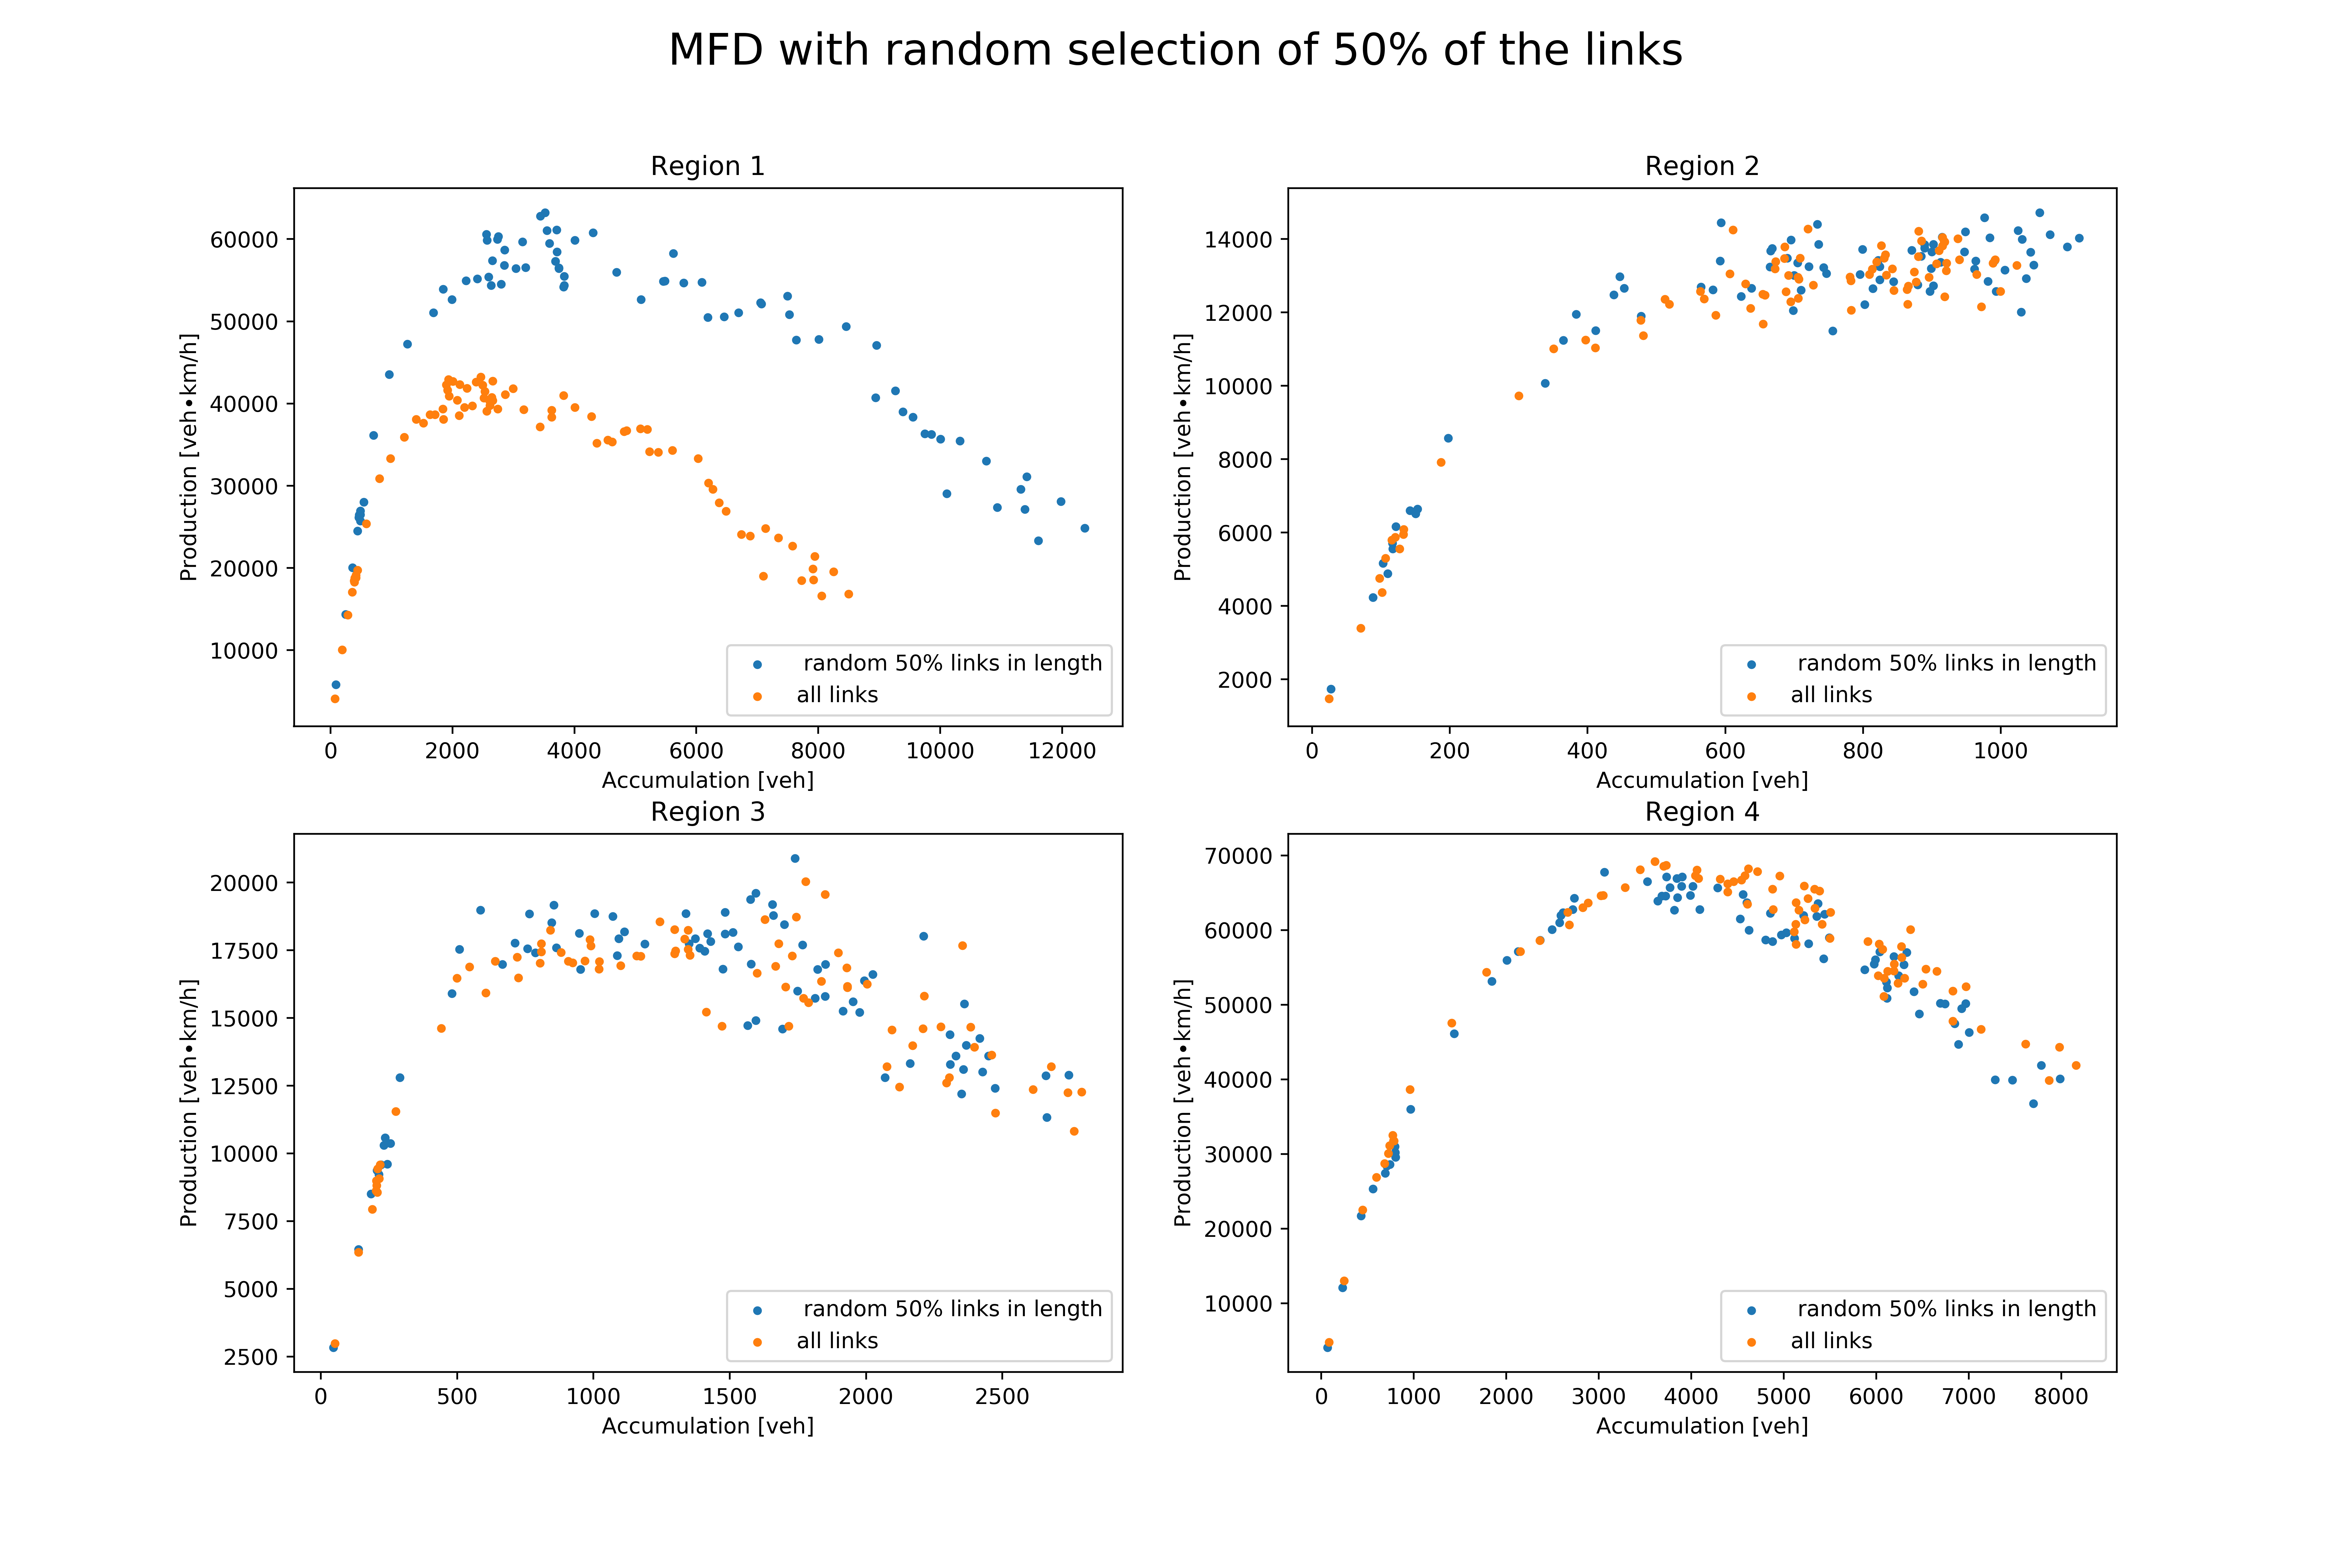
\includegraphics[width=18cm]{Images/step6_random.png}
        \caption{MFD with random selection of 50\% of the links}
        \label{MFD with random selection of 50\% of the links}
    \end{center}
\end{figure}

In this case, the results seem to be good or very good in the different regions, except for region 1. For region 2 in particular, the 50\% of the selected data are very close to reality. Moreover, what is interesting to note is that, contrary to the previous strategy, the biases are not at all constant. For example, for region 1, we find higher values than reality, while for region 4, we find lower values little smaller than reality. This is not necessarily specific to the regions considered but just to the randomness of the data selection, another choice could give different results without anything changing in the real data, just the random choice of the 50\% considered. 
\smallbreak
What would be interesting is to try to keep this relatively uniform aspect in the data selection, while losing the randomness of the last strategy which, although very good in most cases, can lead to false results in very unfavourable data selection situations. Two solutions could then be used in the future and we will develop them. On the one hand, it would be possible to select, for example, one of every two paths in terms of length. This would make it possible to have a fairly uniform distribution, without excluding the tails of distributions, which was the problem of the first strategy. However, the problem may be that the total length will still not be the same as the total length of the links when considering all lanes. On the other hand, in order to counter the last statement, it may be interesting to randomly choose links, but by imposing that the total length of these links is identical to the total length of the network as a whole, it seems possible to arrive at a hybrid solution countering many of the negative situations seen previously.
\bigbreak
Finally, it should be noted that the best way to reduce the error in general would be to proceed by iteration, with an error minimisation algorithm. However, by doing this, it imposes to consider even more data than to consider the whole of the data in the analysis and one loses all the interest of the approach which imposed the use of 50\% of the channels in this case (in order to reduce the computing time in particular). This is why these strategies have not been mentioned throughout this research into minimising the error by considering only 50\% of the links.
Otherwise, in general, we can see that it is absolutely necessary to choose a strategy in correlation with the scale factor. Rather than imposing a constant scaling factor equal to 2, it would probably be simpler to choose a strategy of selecting 50\% of the links in a way, and then choose a scale factor who fits great with the data we choose.




\section{Step 7 - Analysis of heterogeneity}

It is then interesting to study the heterogeneity of the spatial distribution of the density in the network and to analyze the influence of the shape and the noise of the MFD. Furthermore it is possible to study the impact of the distribution of data in different regions. For this purpose, it is possible to plot the spatial distribution of occupancy for the 4 different clusters and the
whole network for times 60min and 90min.
\begin{figure}[H]
    \begin{center}
        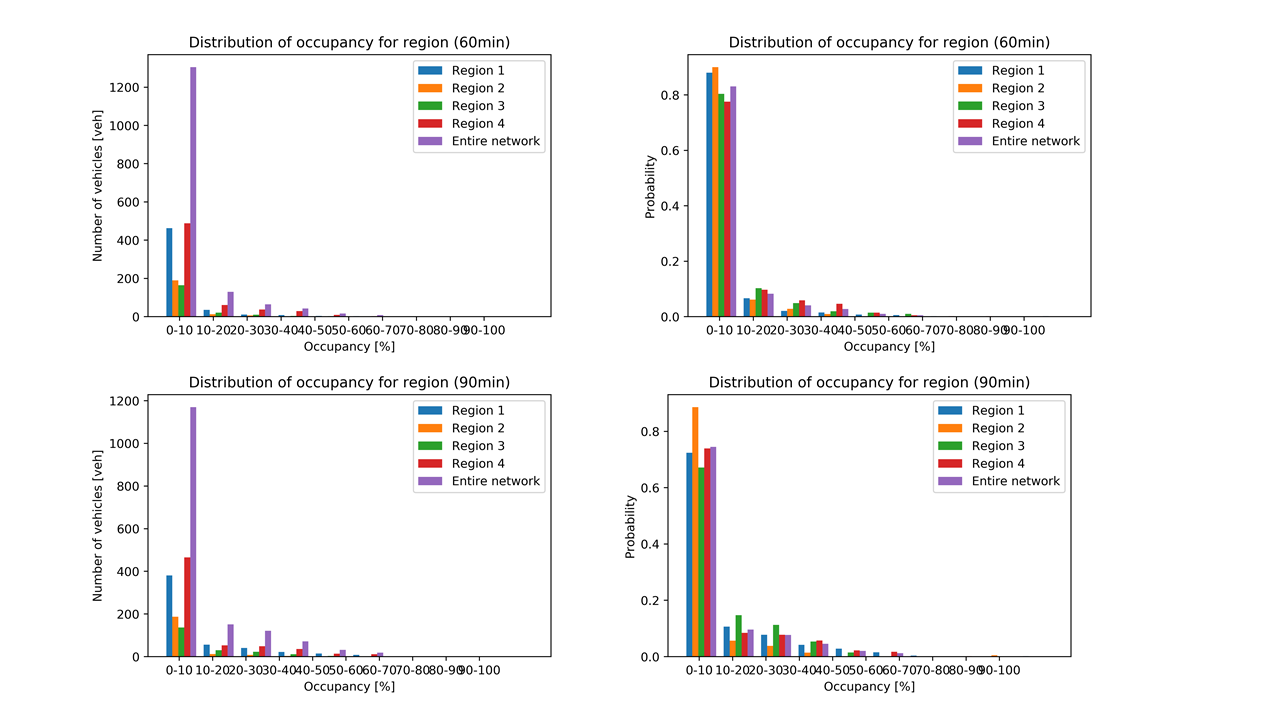
\includegraphics[width=19cm]{Images/Distribution of occupancy for region 4 graphs.png}
        \caption{Distribution of occupancy for regions (60min and 90 min)}
        \label{Distribution of occupancy for region (60min and 90 min)}
    \end{center}
\end{figure}



On these two graphs, it is shown the frequency of occupation according to the different regions. Globally, for the graph at 60min, there seems to be a higher frequency for low occupancy with values around 0.8 against about 0.7 for t=90 min (except region 2). Thus, all regions except 2 are more congested at time 90 min than 60 min. Moreover, region 2 seems less congested than the others. Indeed, all the other regions have relatively similar values, and close to the values for the whole networks.
\bigbreak
In order to estimate the homogeneity of the regions, it may be interesting to calculate the standard deviations and the variance of the occupancy at time 60 and 90 min.


\begin{table}[H]
\begin{center}
\begin{tabular}{|c|c|c|c|c|c|}
\hline   & Region 1 & Region 2 & Region 3 & Region 4 & Entire network \\
\hline t=60 [min] & 10.371 & 6.453 & 10.985 & 12.452 & 11.057 \\
\hline  t=90 [min] & 15.332 & 9.896 & 12.432 & 14.739 & 14.240 \\
\hline
\end{tabular}
\caption{Standard deviation of the occupancy}
\label{Standard deviation of the occupancy}
\end{center}
\end{table}

\begin{table}[H]
\begin{center}
\begin{tabular}{|c|c|c|c|c|c|}
\hline   & Region 1 & Region 2 & Region 3 & Region 4 & Entire network \\
\hline t=60 [min] & 107.562 & 41.638 & 120.670 & 155.043 & 122.261 \\
\hline  t=90 [min] & 235.080 & 97.936 & 154.547& 217.243 & 202.774 \\
\hline
\end{tabular}
\caption{Variance of the occupancy}
\label{Variance of the occupancy}
\end{center}
\end{table}

The separation of the network into several regions has the objective of making it more homogeneous. We would like to check if the separations that have been made here with the four regions really allows to increase the homogeneity in each of them. A region can be considered more homogeneous if the standard deviation of the occupancy of this region is lower than that of the whole network. From the results found, it is possible to say that only region 2 is more homogeneous. Thus the division into four regions as it has been done does not increase the homogeneity except for region 2.\\
It is nevertheless interesting to note that the standard deviation of occupancy is variable over time. Indeed, for the whole network, it goes from 11,057 to 14,240. At t=60 [min], the regions have values relatively close to that of the whole network and even lower for regions 2. Thus the influence of the regions on the homogeneity is not very visible. But at t=90 [min], the standard deviations all increase strongly except for region 2. This strong increase is probably due to the fact that, as presented previously, at t=90 [min], the network is more congested so more variations between the different data and regions.

\bigbreak
In addition to that, it is interesting to calculate a very interesting statistic in transportation in the area of division in region, the TVn. This value shows how the division into different regions has brought a certain homogeneity that would not be present if the whole network were considered in one piece. This value, contained between 0 and 1 is calculated as follows: 

\begin{equation}
       TV_n = \frac{\sum^{N_s}_{i=1}{N_{A_i} \cdot var(A_i) }}{N \cdot var(A)} 
    \label{TV_n}
\end{equation}

where N is the number of link and var(A) the variance parameter of the distribution for region A.\\

The closer this parameter is to 0, the more difference there is in terms of heterogeneity between the regions studied. That is to say that if we find a value close to 0, it was interesting to make a division in region in order to have a certain homogeneity inside these last ones, which we did not have by considering the whole network.
\smallbreak
On the contrary, if we find a value close to 1, it means that there is no great gain in making this division by region in terms of homogeneity. In this case, two explanations are possible. On the one hand, the heterogeneity at the level of the regions can remain almost as great as if we took the whole network. On the other hand, it may also mean that the homogeneity on the global original network was already rather good and that it is not much improved by dividing it by region.
\begin{table}[H]
\begin{center}
\begin{tabular}{|c|c|c|}
\hline    & t=60 [min] & t=90 [min] \\
\hline TVn & 0.977 & 0.981 \\
\hline
\end{tabular}
\caption{TVn at time 60 min and 90 min}
\label{TVn at time 60 min and 90 min}
\end{center}
\end{table}
In our case, we find $TV_n$ close to 1, in these cases, which shows that we do not have a big gain in homogeneity thanks to the division by region. In this case, we see that the whole network is already rather homogeneous (with slight variations for region 2 which explains the very slight increase in homogeneity by dividing by region ($TV_n \ne 1$)) and it is therefore mainly the second explanation mentioned previously that applies. 
\smallbreak
One can then ask oneself why to make a division by region if one increases only slightly the homogeneity. In our case, it is probably related to the desire to achieve a Perimeter Control, which requires a control at the borders of the different regions. The division into regions has therefore an explanation, despite the fact that it does not increase the homogeneity much 


\newpage
\section*{Conclusion}
\addcontentsline{toc}{section}{Conclusion}

The objective of this work was to analyze the urban network on the basis of traffic data that could be measured.\\

The data was collected over several hours, which allows an analysis over time and thus to study the evolution of congestion in the city. Although it would be interesting to carry out this work over a longer period of time in order to have more significant results.\\

The city network was divided into four regions in order to make the analysis as homogeneous as possible. By observing the results between these different areas, it was possible to provide more precise information about the traffic situation. Indeed, it was noticed that region 2 was the least congested with lower traffic density and region 1 the most congested.\\

A production analysis was also performed in each region. It was found that the evolution of volume with occupancy was the same as that of production with accumulation.\\

Then, in order to reduce the number of data to be processed, it was suggested to study different strategies to select a part of the data in order to have a sufficiently representative sample of the whole data. Taking the data according to the length of the links allows to have a relatively representative data set.\\

The homogeneity of the regions was also evaluated and except for region 2, the regions as separated do not provide any homogeneity with respect to the whole network.

\end{document}
